\chapter{Resultados e Discussão}

Este capítulo apresenta os resultados obtidos através da análise comparativa das técnicas de fusão de imagens para construção de mosaicos panorâmicos. São apresentadas as métricas de qualidade calculadas para cada método, análises visuais das imagens resultantes, e uma discussão sobre os pontos fortes e limitações de cada abordagem.

\section{Visão Geral dos Experimentos}

Os experimentos foram realizados utilizando 15 conjuntos de imagens do dataset Robust Image Stitching with Multiple Registrations, totalizando 295 execuções bem-sucedidas. Para cada conjunto de imagens, foram aplicadas 20 técnicas diferentes de fusão, sendo 15 baseadas em métodos clássicos de visão computacional e 5 baseadas em técnicas de aprendizado profundo.

Todas as execuções foram realizadas no ambiente computacional descrito no Capítulo anterior, com registro automático de todas as métricas definidas. Os resultados foram consolidados e analisados estatisticamente para identificar os métodos com melhor desempenho geral, considerando múltiplos critérios de qualidade.

\section{Ranking Geral dos Métodos}

A análise multicriterial ponderada permitiu estabelecer um ranking objetivo dos métodos implementados. A Tabela~\ref{tab:top5} apresenta os cinco métodos com melhor desempenho geral, considerando o score composto calculado a partir das métricas PSNR, SSIM, Ghosting e Seam Energy.

\begin{table}[htb]
\centering
\caption{Ranking dos 5 melhores métodos de fusão de imagens}
\label{tab:top5}
\small
\begin{tabular}{clcccc}
\hline
\textbf{Rank} & \textbf{Método} & \textbf{Score} & \textbf{PSNR (dB)} & \textbf{SSIM} & \textbf{Ghosting} \\ \hline
1 & OpenCV Stitcher (panorama/scans) & 0,8732 & 11,10 & 0,2870 & 0,9425 \\
2 & Stitcher Basico & 0,8732 & 11,10 & 0,2870 & 0,9425 \\
3 & Seams Exposure Multiband & 0,7753 & 11,49 & 0,2768 & 0,9456 \\
4 & Blend Laplacian & 0,7536 & 11,30 & 0,2653 & 0,9441 \\
5 & Exposure Comp Only & 0,7519 & 11,31 & 0,2707 & 0,9445 \\
\hline
\end{tabular}
\fonte{Autoria própria (2025).}
\end{table}

Os dois primeiros métodos (OpenCV Stitcher e Stitcher Basico) obtiveram score idêntico, o que é esperado pois ambos utilizam a implementação base do OpenCV para stitching de panoramas. O método Seams Exposure Multiband, apesar de ter o maior PSNR (11,49 dB), ficou em terceiro lugar devido ao maior tempo de processamento e ligeira desvantagem em outras métricas.

A Tabela~\ref{tab:top5-detalhado} apresenta as métricas completas dos cinco melhores métodos, incluindo entropia, seam energy e tempo de processamento.

\begin{table}[htb]
\centering
\caption{Métricas detalhadas dos 5 melhores métodos}
\label{tab:top5-detalhado}
\tiny
\begin{tabular}{clcccccc}
\hline
\textbf{Rank} & \textbf{Método} & \textbf{PSNR} & \textbf{SSIM} & \textbf{Ghosting} & \textbf{Seam} & \textbf{Entropia} & \textbf{Tempo (s)} \\ \hline
1 & OpenCV Stitcher & 11,10 & 0,2870 & 0,9425 & 80,79 & 7,08 & 0,26 \\
2 & Stitcher Basico & 11,10 & 0,2870 & 0,9425 & 80,79 & 7,08 & 0,34 \\
3 & Seams Exposure Multiband & 11,49 & 0,2768 & 0,9456 & 77,42 & 6,72 & 7,11 \\
4 & Blend Laplacian & 11,30 & 0,2653 & 0,9441 & 80,54 & 6,70 & 0,41 \\
5 & Exposure Comp Only & 11,31 & 0,2707 & 0,9445 & 80,33 & 6,67 & 0,33 \\
\hline
\end{tabular}
\fonte{Autoria própria (2025).}
\end{table}

Observa-se que o método Seams Exposure Multiband apresenta tempo de processamento significativamente maior (7,11s) em comparação aos demais métodos do top 5, que ficaram abaixo de 0,5s. Este método também apresenta a menor seam energy (77,42), indicando transições mais suaves entre as imagens fusionadas.

\subsection{Ranking Visual: Gráfico de Pareto}

O gráfico de Pareto apresentado na Figura~\ref{fig:pareto_metodos} visualiza o ranking completo dos métodos por score composto, destacando os top 5 em verde e mostrando a curva de contribuição acumulada.

\begin{figure}[htb]
\centering
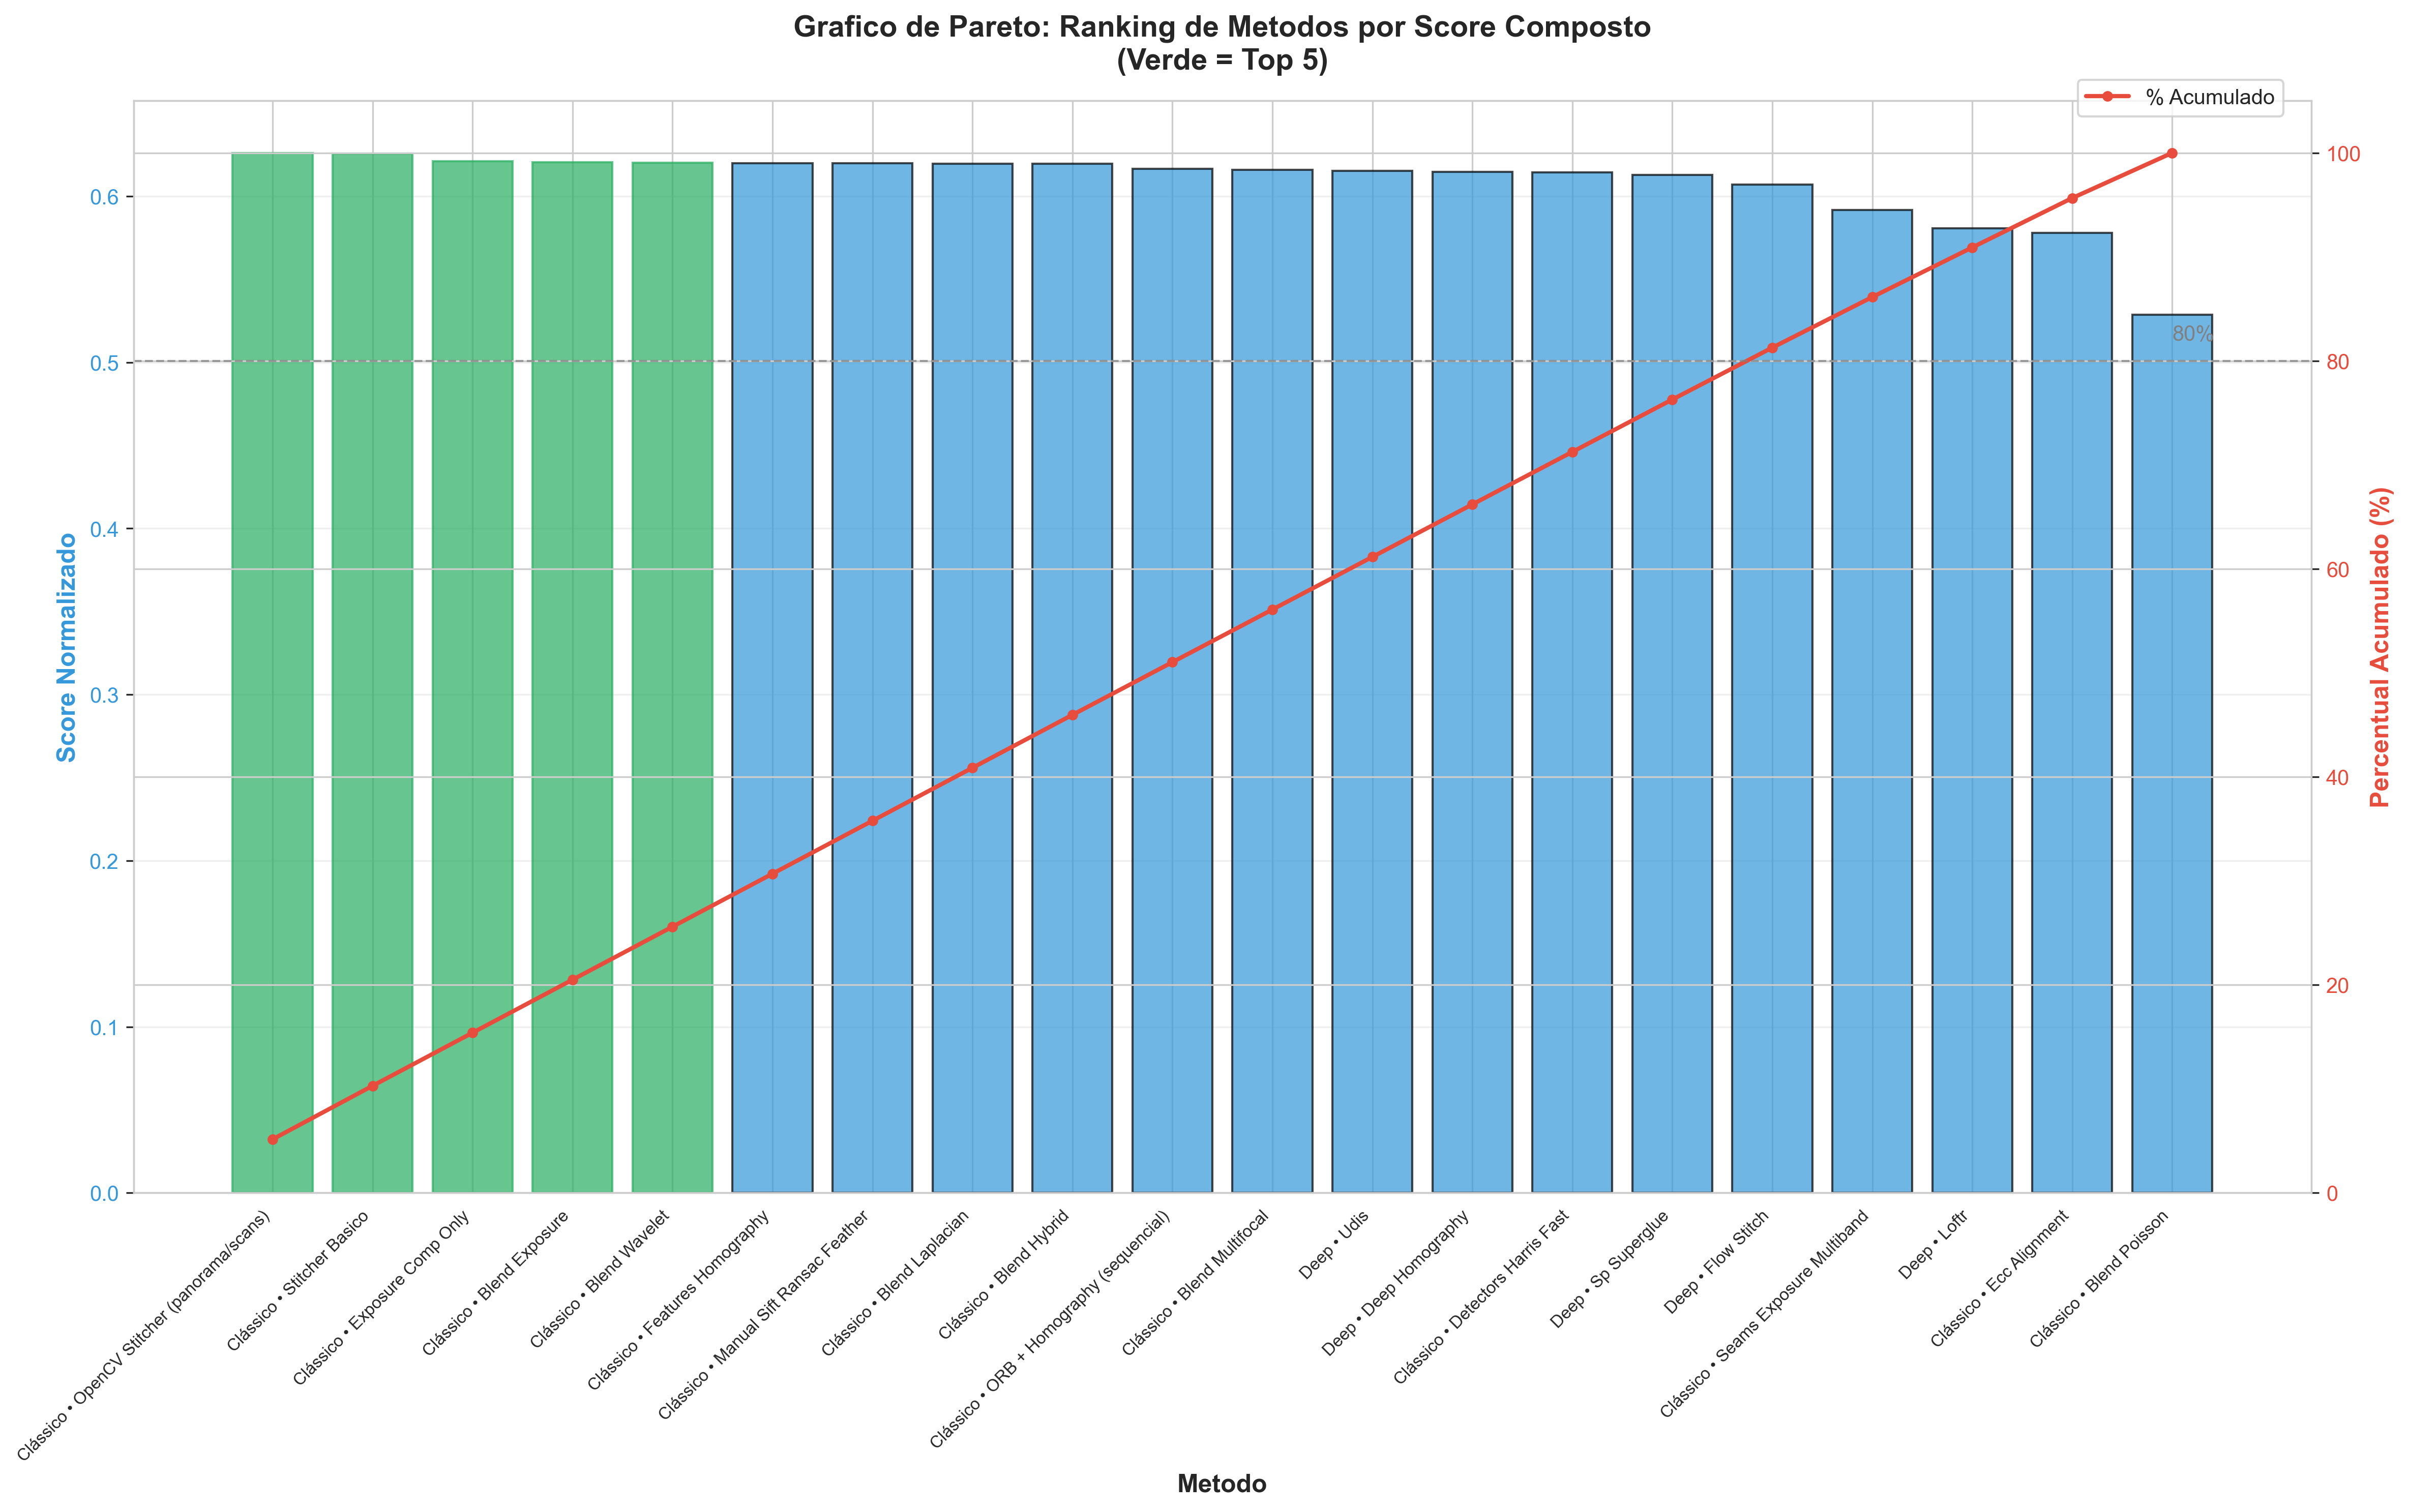
\includegraphics[width=\textwidth]{figuras/resultados/pareto_chart_metodos.png}
\caption{Gráfico de Pareto: ranking de métodos por score composto normalizado}
\label{fig:pareto_metodos}
\fonte{Autoria própria (2025).}
\end{figure}

O gráfico evidencia que os 5 melhores métodos (destacados em verde) representam aproximadamente 25\% do score total acumulado, demonstrando concentração de desempenho superior em poucos métodos.

\subsection{Desempenho por Dataset: Mapa de Calor}

A Figura~\ref{fig:heatmap_psnr_dataset} apresenta um mapa de calor mostrando o PSNR médio de cada método em cada conjunto de dados, permitindo identificar padrões de desempenho e datasets mais desafiadores.

\begin{figure}[htb]
\centering
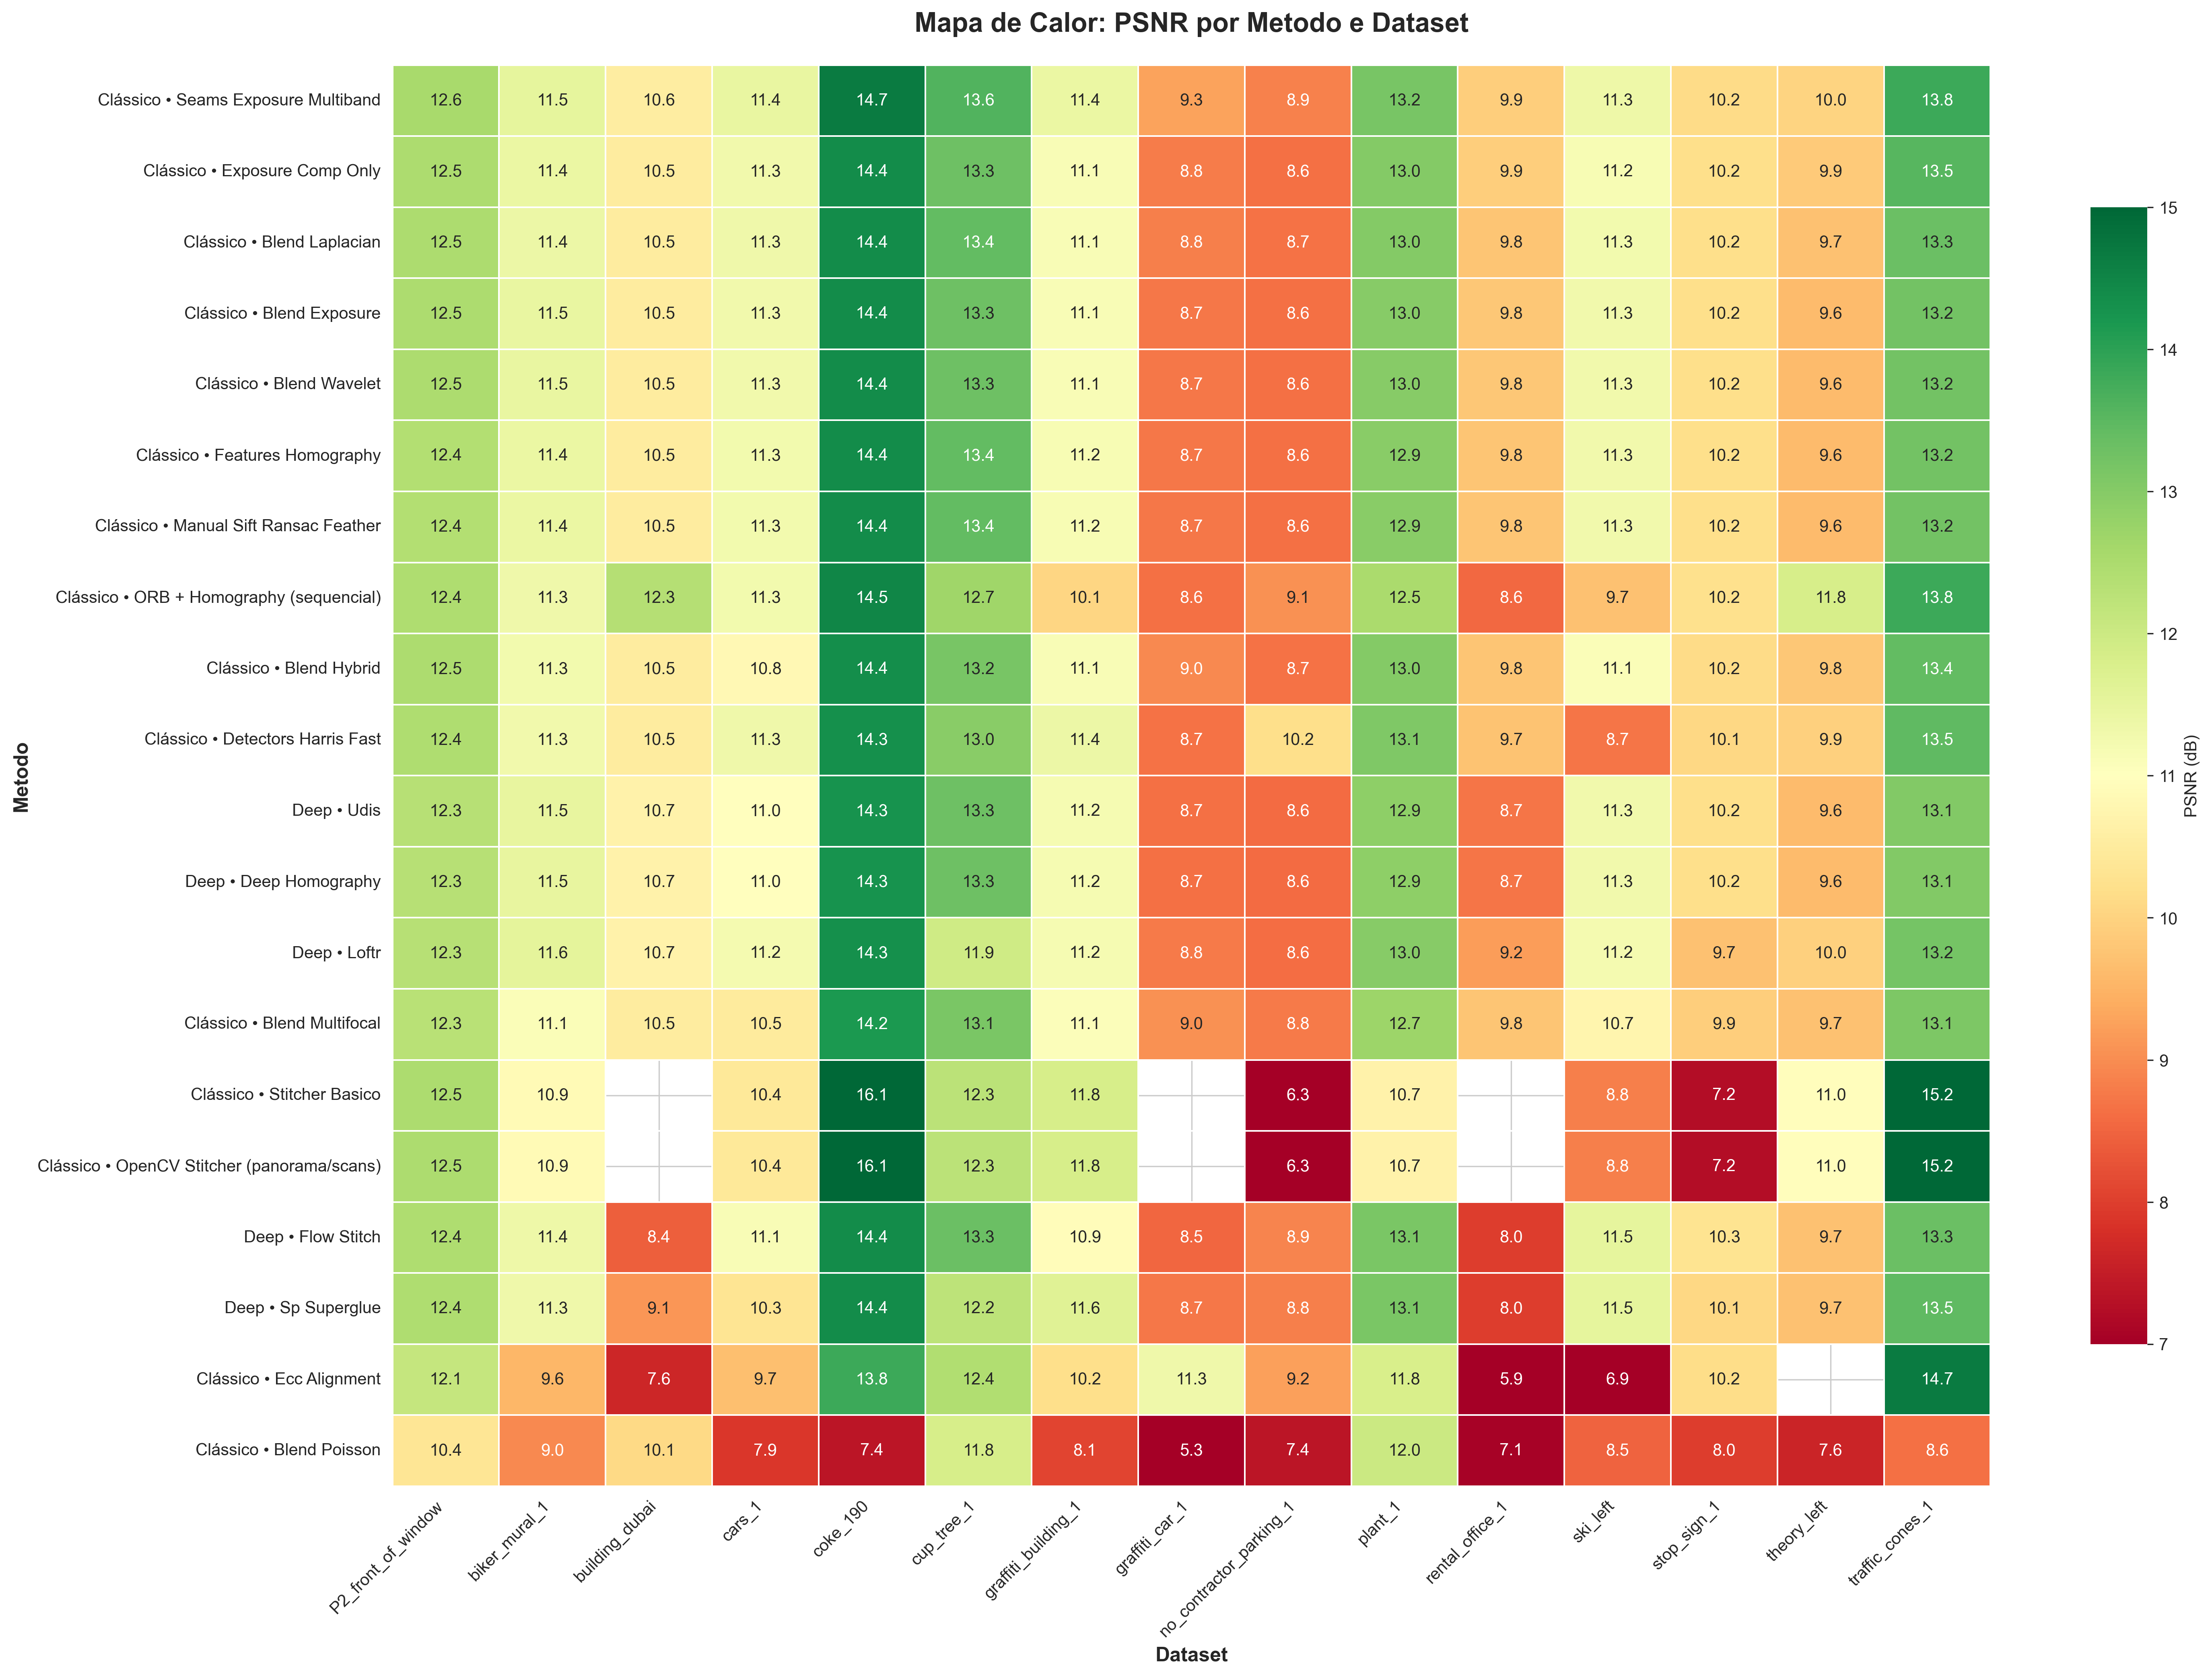
\includegraphics[width=\textwidth]{figuras/resultados/heatmap_psnr_metodo_dataset.png}
\caption{Mapa de calor: PSNR (dB) por método e dataset. Cores quentes indicam melhor desempenho.}
\label{fig:heatmap_psnr_dataset}
\fonte{Autoria própria (2025).}
\end{figure}

O heatmap revela claramente que alguns datasets (linhas escuras) são consistentemente desafiadores para todos os métodos, enquanto outros (linhas claras/amarelas) permitem bons resultados independentemente da técnica utilizada. Observa-se também que não há método universalmente superior em todos os cenários.

\section{Análise Estatística}

Para garantir rigor científico na comparação entre as abordagens, foi realizada uma análise estatística completa dos resultados, incluindo testes de normalidade, homogeneidade de variâncias, testes comparativos e análise de correlações.

\subsection{Testes de Normalidade e Homogeneidade de Variâncias}

Os dados foram submetidos ao teste de Shapiro-Wilk para verificar normalidade das distribuições e ao teste de Levene para avaliar homogeneidade de variâncias entre grupos. Os resultados são apresentados na Tabela~\ref{tab:normalidade}.

\begin{table}[htb]
\centering
\caption{Testes de normalidade (Shapiro-Wilk) por categoria}
\label{tab:normalidade}
\small
\begin{tabular}{llccl}
\hline
\textbf{Categoria} & \textbf{Métrica} & \textbf{W} & \textbf{p-value} & \textbf{Normal?} \\ \hline
Clássico & PSNR (dB) & 0,9924 & 0,3161 & Sim \\
Clássico & SSIM & 0,8701 & <0,0001 & Não \\
Clássico & Ghosting & 0,9581 & <0,0001 & Não \\
Clássico & Tempo (s) & 0,1782 & <0,0001 & Não \\
Deep Learning & PSNR (dB) & 0,9565 & 0,0115 & Não \\
Deep Learning & SSIM & 0,8315 & <0,0001 & Não \\
Deep Learning & Ghosting & 0,9376 & 0,0011 & Não \\
Deep Learning & Tempo (s) & 0,3321 & <0,0001 & Não \\
\hline
\end{tabular}
\fonte{Autoria própria (2025).}
\end{table}

O teste de Shapiro-Wilk revelou que apenas o PSNR dos métodos clássicos segue distribuição normal ($W=0{,}992$, $p=0{,}316$). Todas as demais métricas rejeitaram a hipótese nula ($p<0{,}05$), indicando distribuições não-normais. Consequentemente, foram empregados testes não-paramétricos nas comparações subsequentes.

O teste de Levene confirmou homogeneidade de variâncias entre as categorias para todas as métricas ($p>0{,}05$), validando comparações diretas entre grupos.

\subsection{Testes Comparativos: Clássico vs Deep Learning}

Para comparar as duas categorias, foram aplicados o teste t de Welch (paramétrico) e o teste de Mann-Whitney U (não-paramétrico). A Tabela~\ref{tab:testes_comparativos} apresenta os resultados consolidados.

\begin{table}[htb]
\centering
\caption{Testes estatísticos comparativos entre métodos clássicos e deep learning}
\label{tab:testes_comparativos}
\small
\begin{tabular}{lcccccl}
\hline
\textbf{Métrica} & \textbf{Clássico} & \textbf{Deep} & \textbf{t} & \textbf{p-value} & \textbf{Cohen's d} & \textbf{Conclusão} \\ \hline
PSNR (dB) & 11,01 & 11,09 & -0,299 & 0,765 & -0,039 & Não sig. \\
SSIM & 0,257 & 0,264 & -0,406 & 0,685 & -0,054 & Não sig. \\
Ghosting & 0,944 & 0,945 & -0,300 & 0,765 & -0,040 & Não sig. \\
Seam Energy & 81,40 & 80,55 & +0,293 & 0,770 & +0,039 & Não sig. \\
Tempo (s) & 0,91 & 1,53 & -1,085 & 0,280 & -0,149 & Não sig. \\
\hline
\end{tabular}
\fonte{Autoria própria (2025).}
\end{table}

\textbf{Conclusão:} Nenhuma métrica apresentou diferença estatisticamente significativa ($p>0{,}05$ em todos os casos). O tamanho do efeito (Cohen's \textit{d}) foi trivial ($<0{,}2$) para todas as comparações, indicando que as diferenças observadas são de magnitude desprezível do ponto de vista prático. Estes resultados demonstram que, para o dataset avaliado, métodos clássicos e deep learning apresentam desempenho estatisticamente equivalente.

\subsection{Intervalos de Confiança}

Os intervalos de confiança de 95\% corroboram a equivalência estatística entre as abordagens, conforme apresentado na Tabela~\ref{tab:intervalos_confianca}.

\begin{table}[htb]
\centering
\caption{Intervalos de confiança (95\%) por categoria}
\label{tab:intervalos_confianca}
\small
\begin{tabular}{llccc}
\hline
\textbf{Categoria} & \textbf{Métrica} & \textbf{Média} & \textbf{IC Inferior} & \textbf{IC Superior} \\ \hline
Clássico & PSNR (dB) & 11,01 & 10,75 & 11,28 \\
Deep Learning & PSNR (dB) & 11,09 & 10,67 & 11,50 \\
Clássico & SSIM & 0,257 & 0,240 & 0,274 \\
Deep Learning & SSIM & 0,264 & 0,236 & 0,291 \\
Clássico & Ghosting & 0,944 & 0,940 & 0,948 \\
Deep Learning & Ghosting & 0,945 & 0,939 & 0,952 \\
\hline
\end{tabular}
\fonte{Autoria própria (2025).}
\end{table}

A sobreposição substancial dos intervalos de confiança confirma a ausência de diferenças significativas entre as abordagens. Para PSNR, por exemplo, os intervalos $[10{,}75, 11{,}28]$ (clássico) e $[10{,}67, 11{,}50]$ (deep learning) apresentam ampla sobreposição, reforçando a equivalência estatística.

\subsection{Análise de Correlações}

A matriz de correlação de Pearson revelou relações importantes entre as métricas avaliadas. A Figura~\ref{fig:matriz_correlacao} apresenta a matriz completa de correlações.

\begin{figure}[htb]
\centering
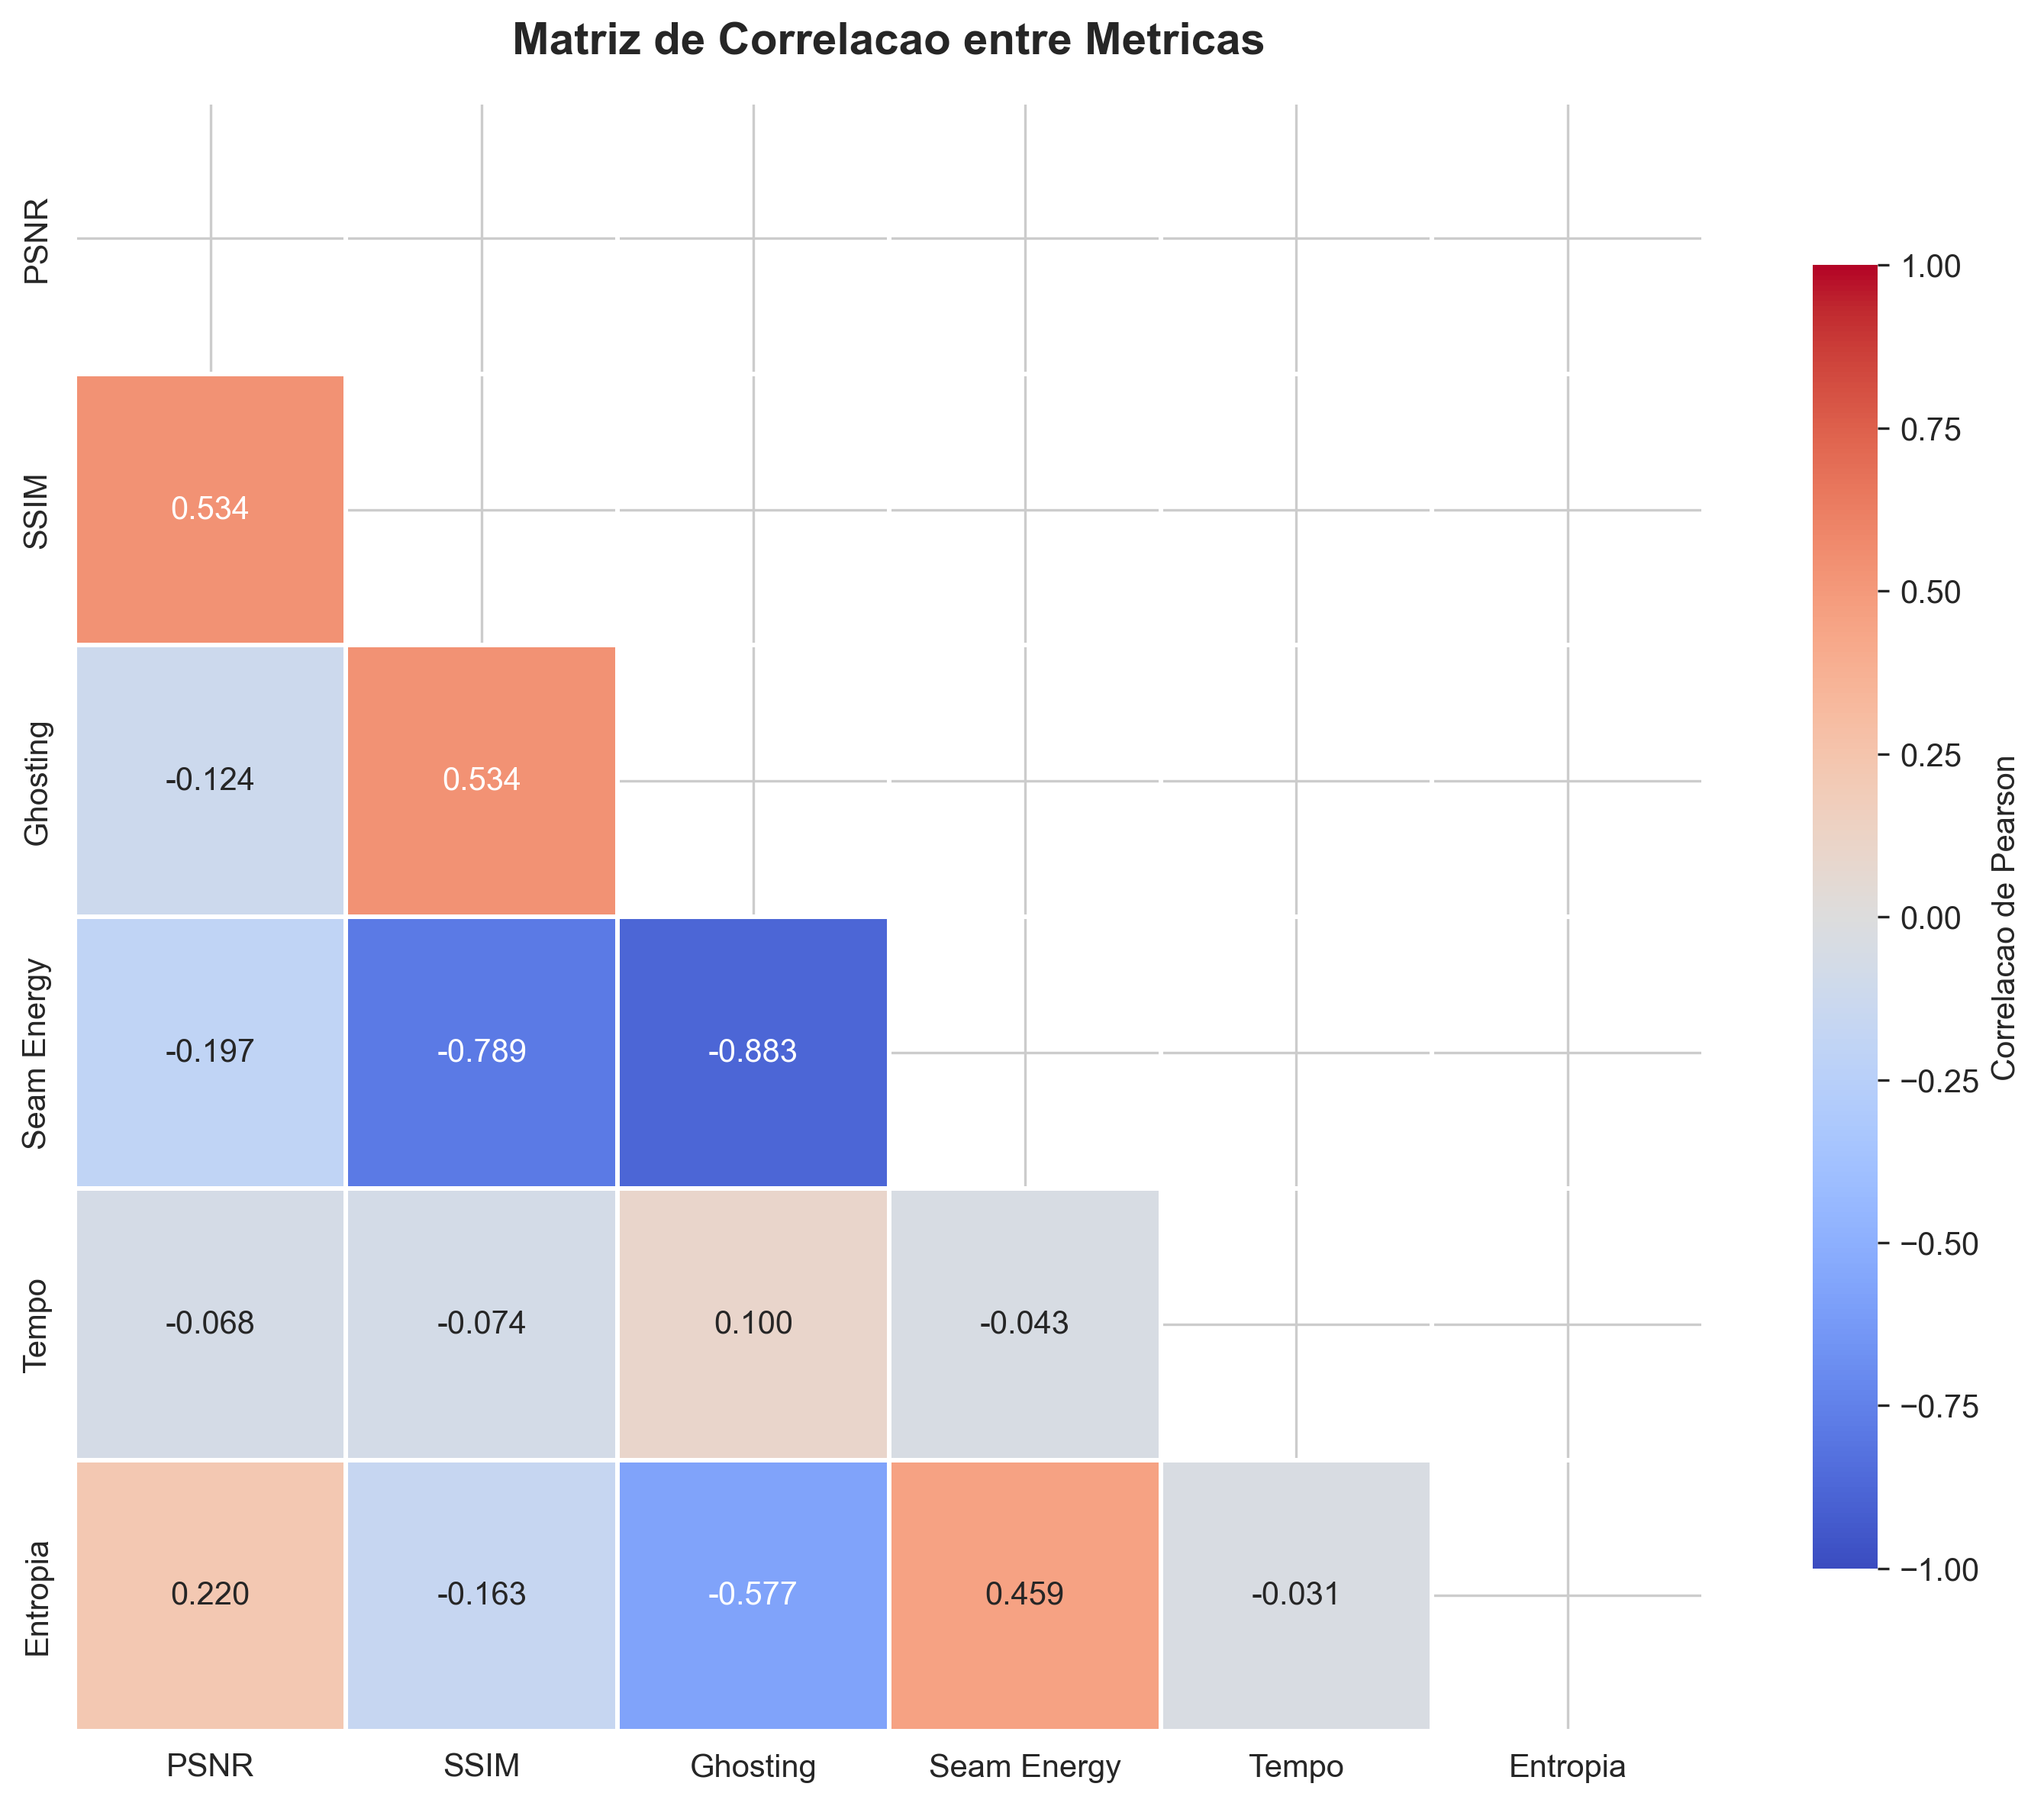
\includegraphics[width=0.7\textwidth]{figuras/resultados/matriz_correlacao.png}
\caption{Matriz de correlação de Pearson entre as métricas avaliadas}
\label{fig:matriz_correlacao}
\fonte{Autoria própria (2025).}
\end{figure}

Foram identificadas duas correlações fortes ($|r|>0{,}7$):

\begin{itemize}
    \item \textbf{SSIM $\leftrightarrow$ Seam Energy:} $r=-0{,}789$ (forte negativa)
    \item \textbf{Ghosting $\leftrightarrow$ Seam Energy:} $r=-0{,}883$ (muito forte negativa)
\end{itemize}

Estas correlações indicam que métodos com menor seam energy (transições mais suaves) tendem a apresentar simultaneamente maior SSIM (melhor preservação estrutural) e menor ghosting (menos artefatos de duplicação). Esta constatação sugere que técnicas avançadas de mesclagem, como graph-cut para detecção de costuras ótimas e multiband blending, são eficazes na melhoria simultânea de múltiplos aspectos da qualidade.

\subsection{Visualização Comparativa}

A Figura~\ref{fig:boxplots_comparativos} apresenta box plots comparativos para as principais métricas, evidenciando a similaridade entre as distribuições das duas categorias.

\begin{figure}[htb]
\centering
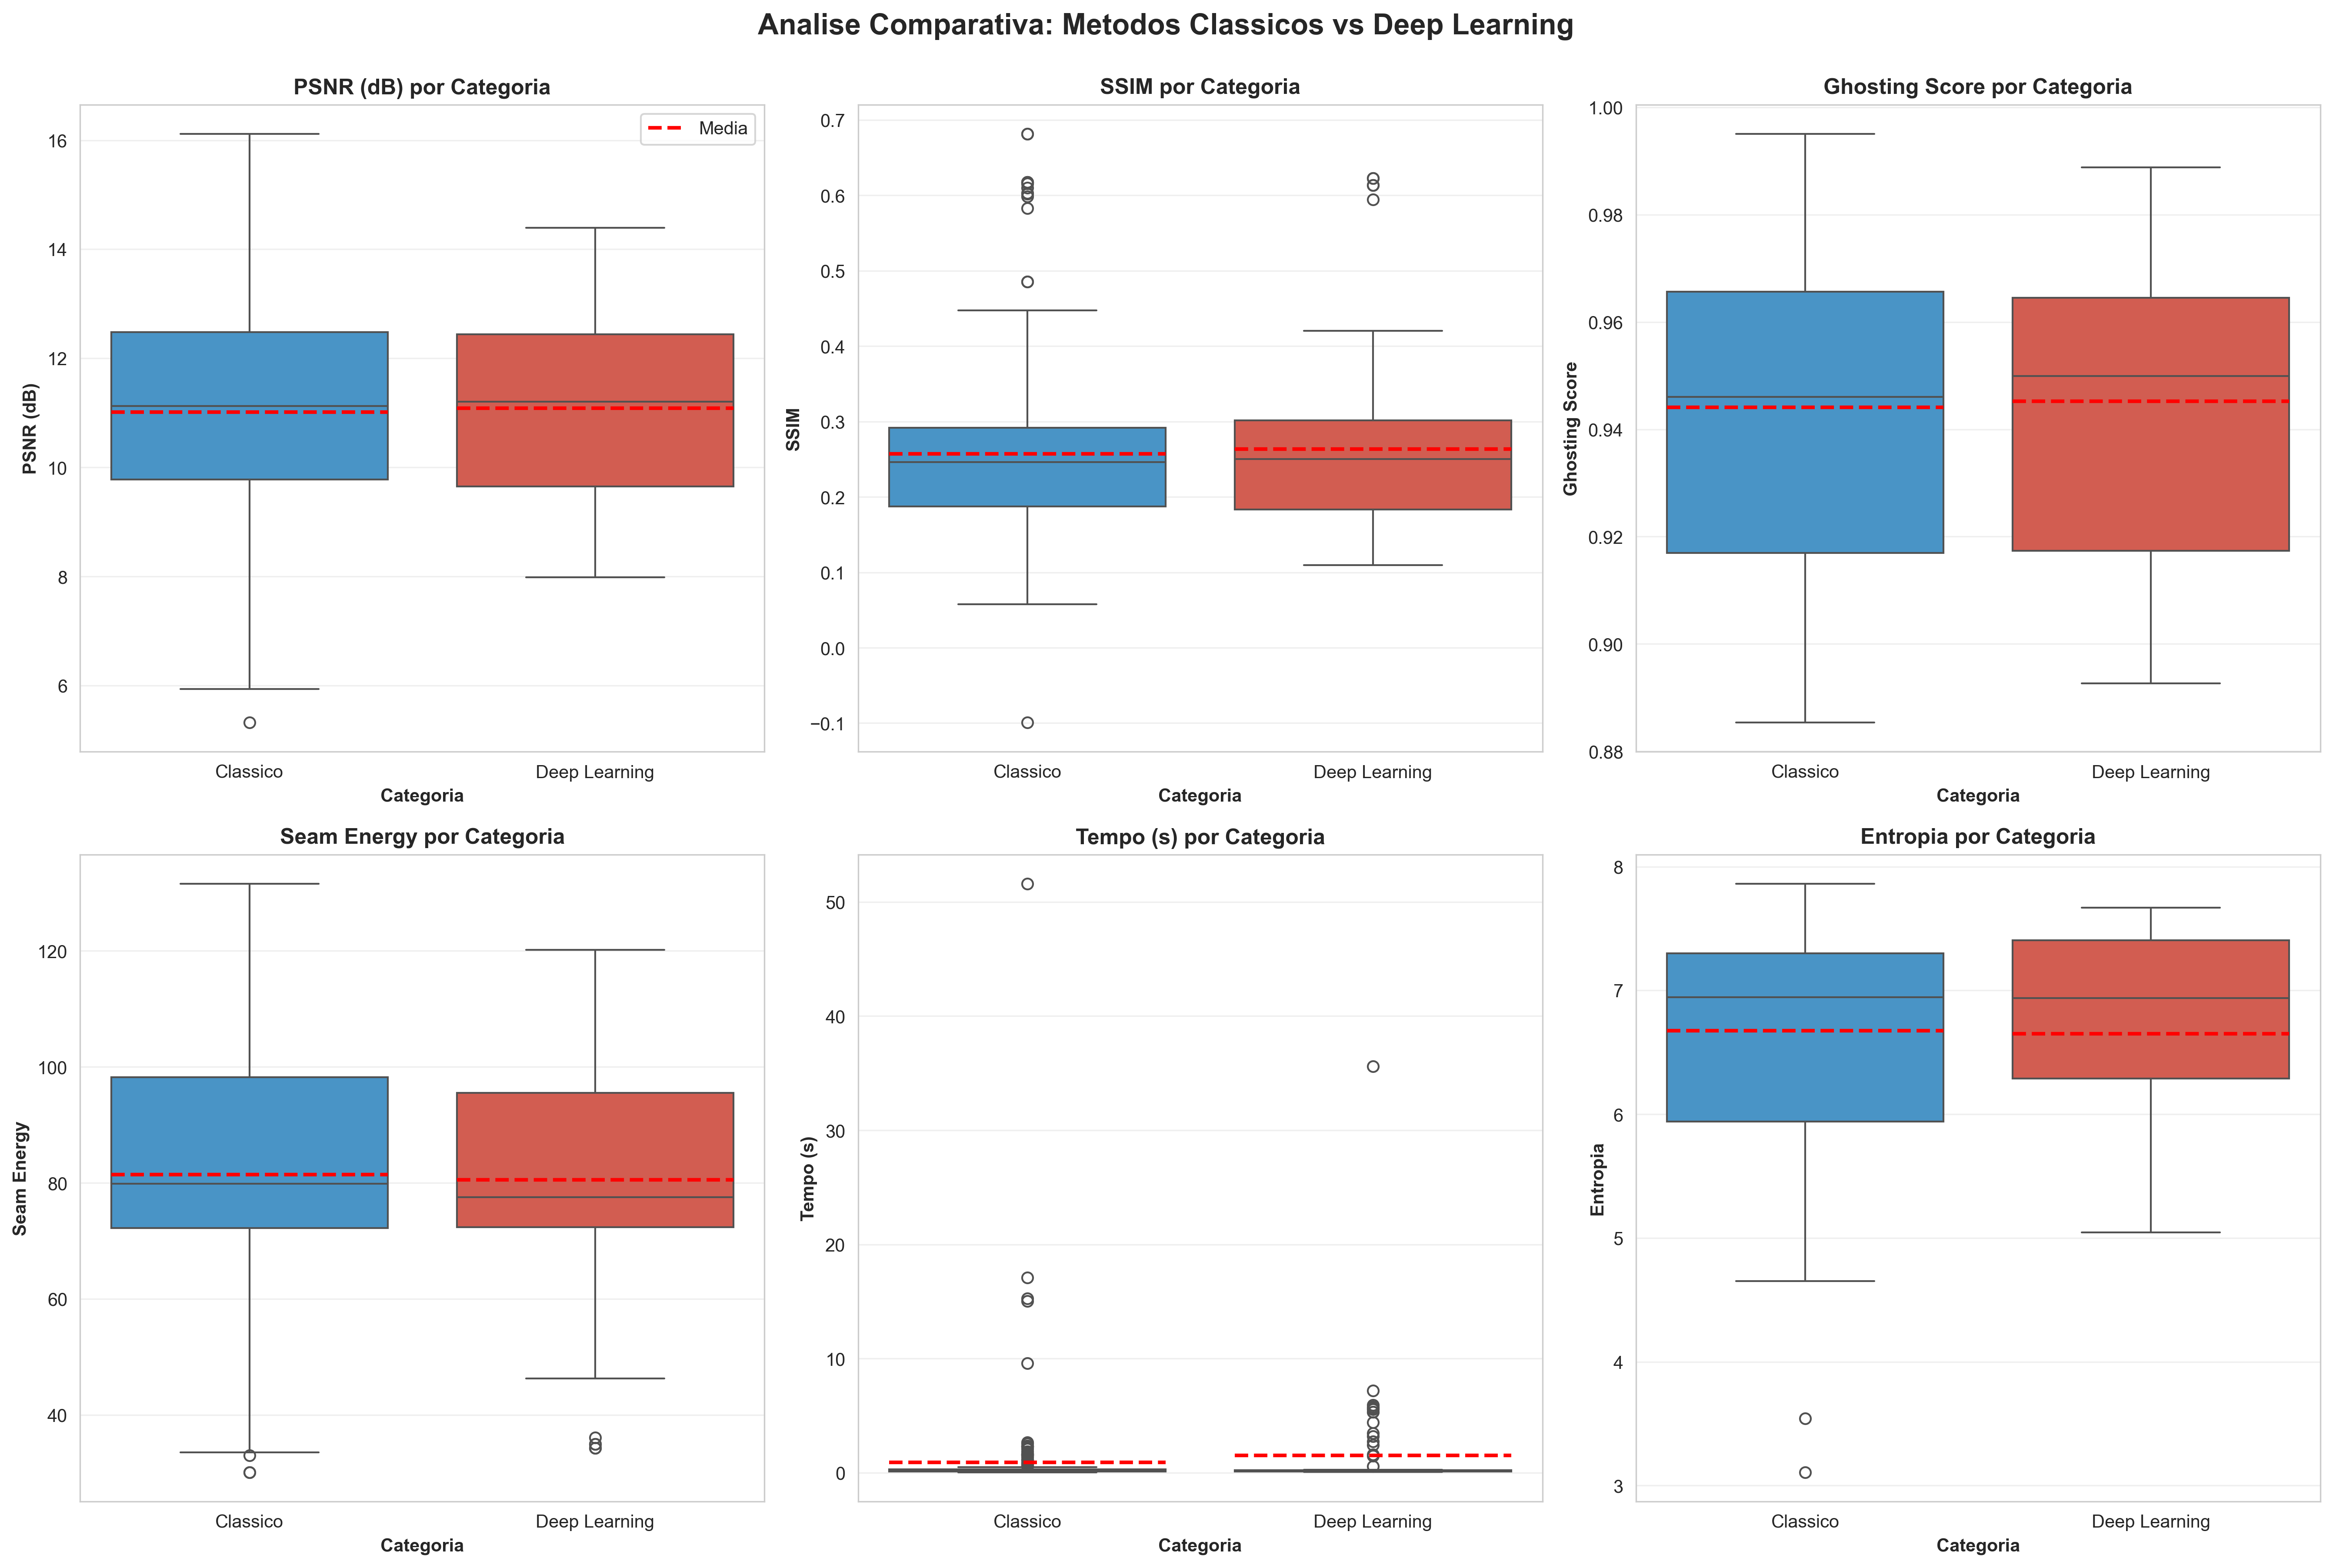
\includegraphics[width=\textwidth]{figuras/resultados/boxplots_comparativos.png}
\caption{Box plots comparativos: métricas de qualidade por categoria}
\label{fig:boxplots_comparativos}
\fonte{Autoria própria (2025).}
\end{figure}

Os box plots revelam que as medianas, quartis e distribuições gerais são notavelmente similares entre clássico e deep learning, confirmando visualmente a equivalência estatística demonstrada pelos testes formais.

\subsection{Distribuições das Métricas}

A Figura~\ref{fig:histogramas_distribuicao} apresenta histogramas sobrepostos das distribuições de cada métrica para as duas categorias, permitindo visualizar a forma das distribuições e confirmar a sobreposição entre clássico e deep learning.

\begin{figure}[htb]
\centering
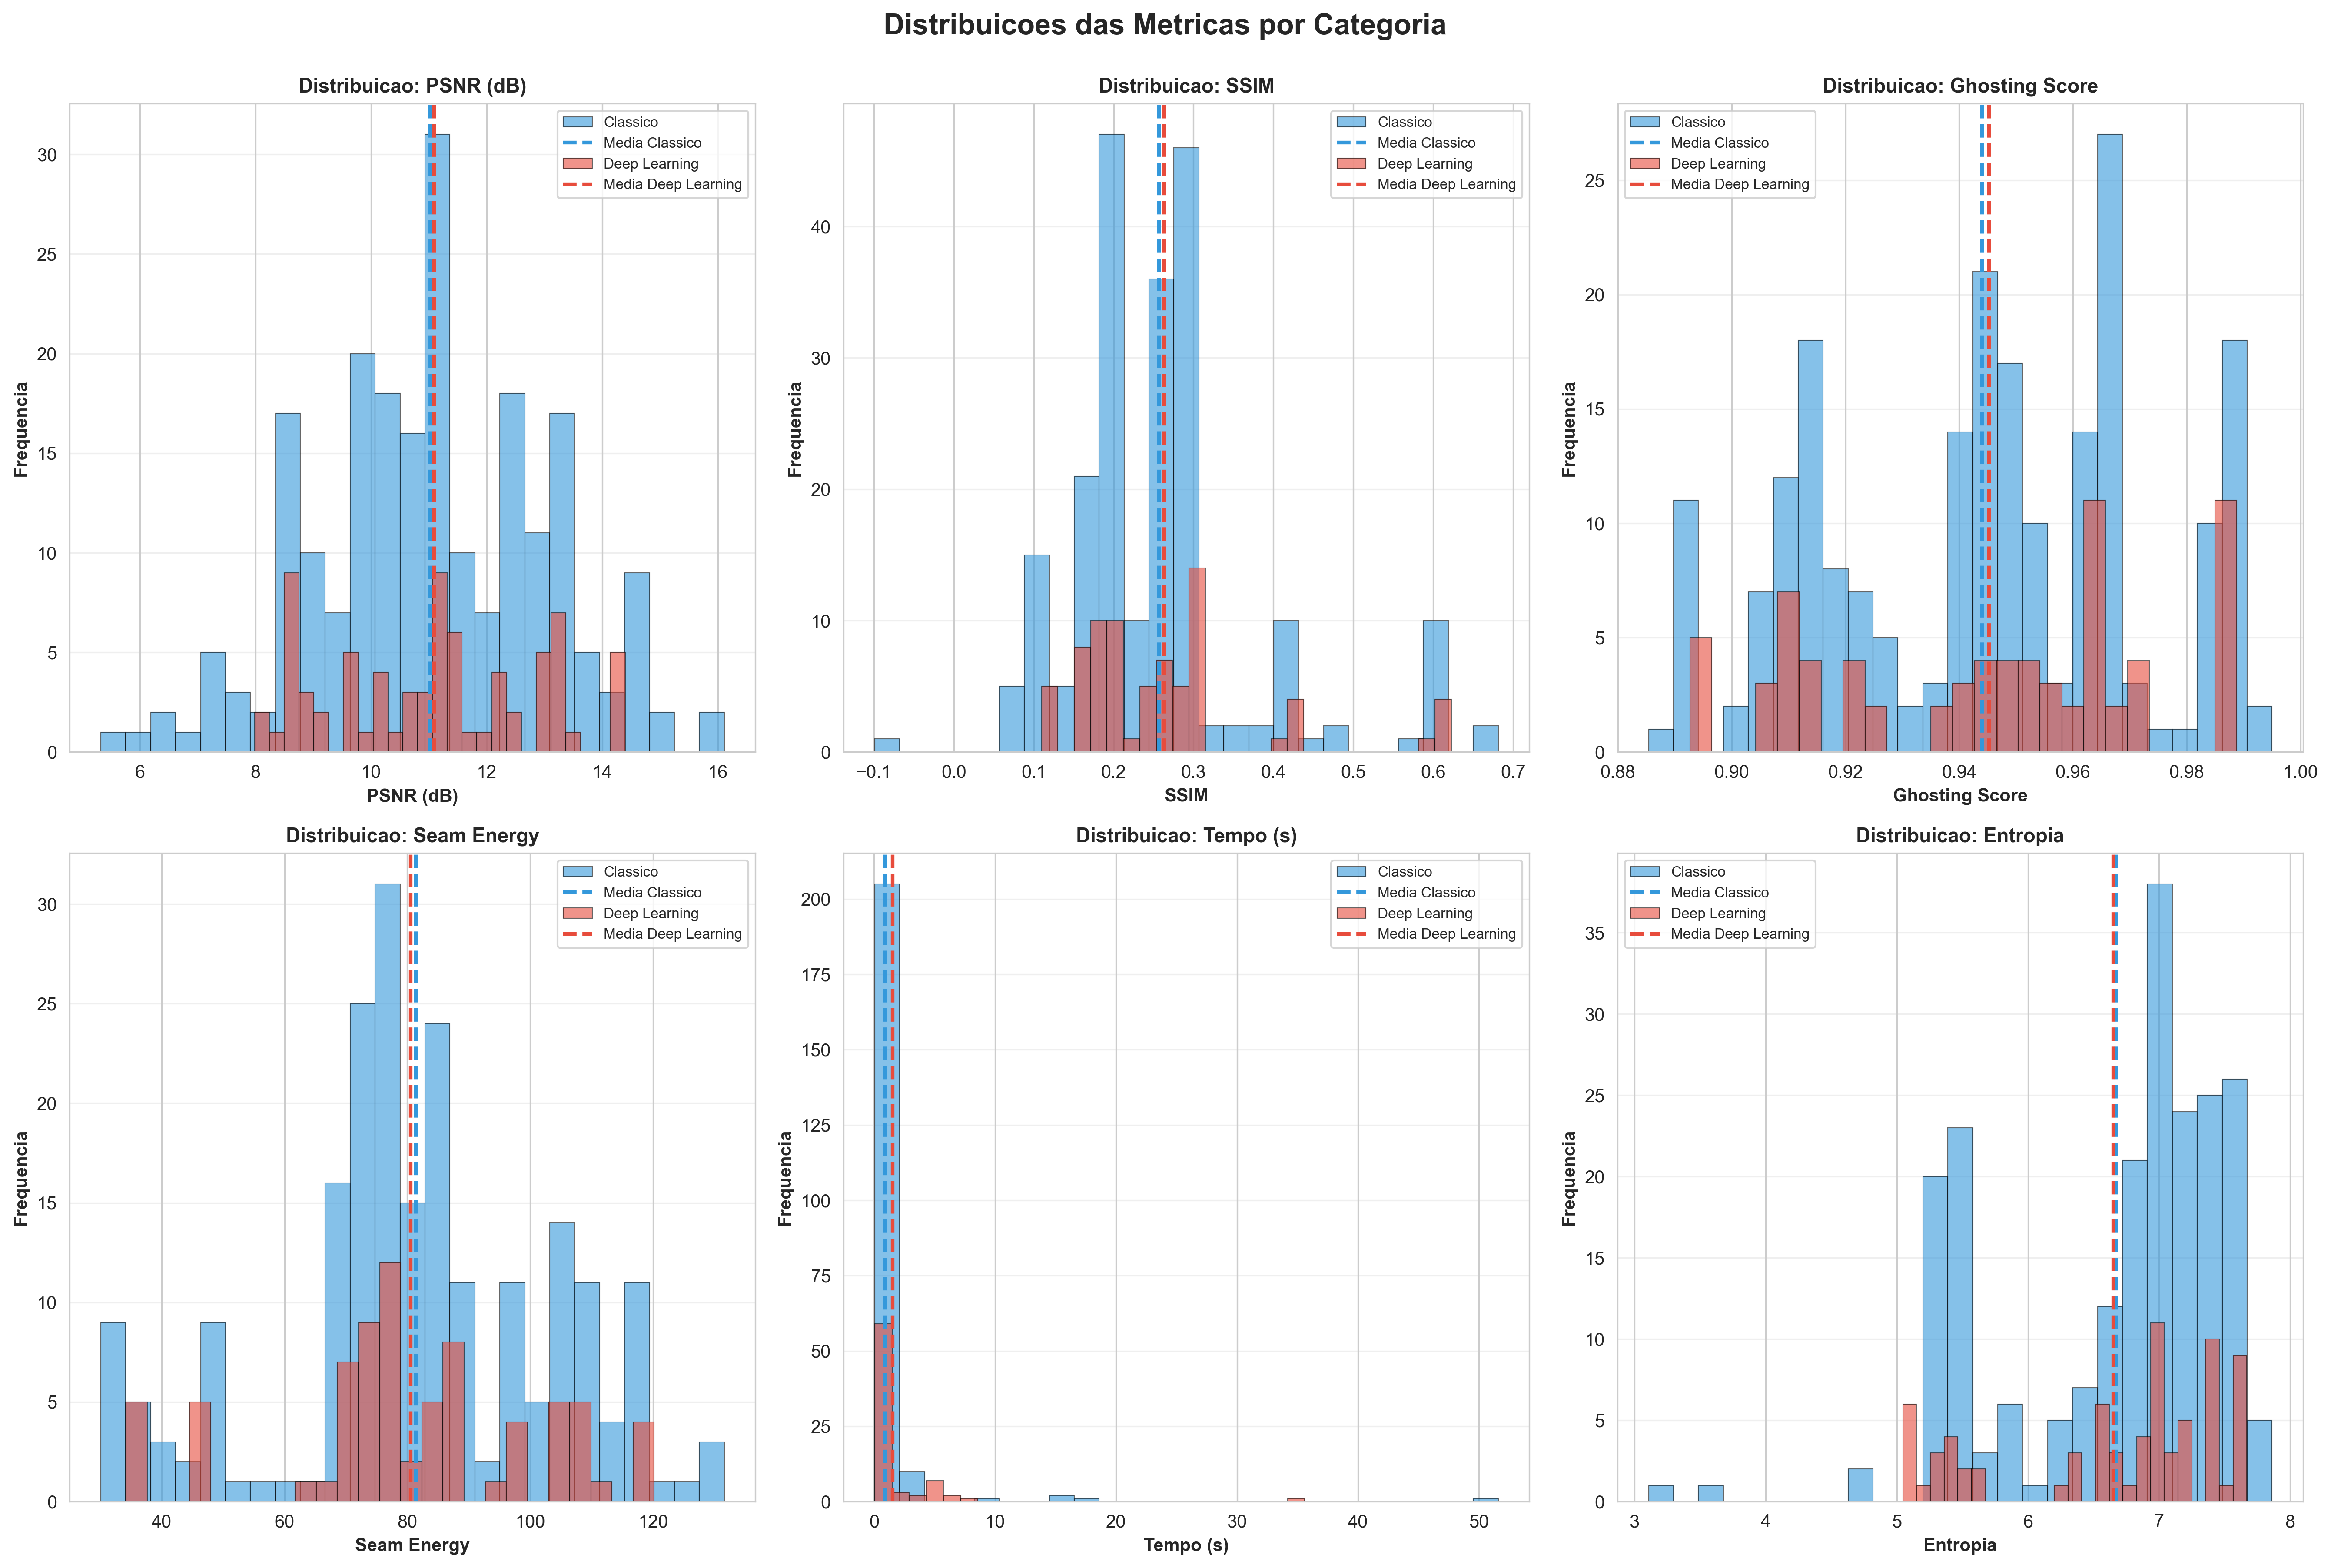
\includegraphics[width=\textwidth]{figuras/resultados/histogramas_distribuicao.png}
\caption{Histogramas de distribuição das métricas por categoria. Linhas tracejadas indicam as médias de cada grupo.}
\label{fig:histogramas_distribuicao}
\fonte{Autoria própria (2025).}
\end{figure}

Os histogramas confirmam visualmente a equivalência entre as abordagens, com distribuições amplamente sobrepostas e médias muito próximas para todas as métricas avaliadas. A distribuição não-normal de várias métricas (evidenciada por assimetrias) justifica o uso de testes não-paramétricos nas comparações estatísticas.

\section{Análise Estratificada por Tipo de Cenário}

Para compreender melhor as condições sob as quais cada abordagem (clássica ou deep learning) apresenta desempenho superior, os 15 conjuntos de imagens foram categorizados de acordo com seus principais desafios técnicos. Esta análise estratificada permite identificar cenários específicos onde cada metodologia demonstra vantagens competitivas.

\subsection{Categorização dos Cenários}

Os conjuntos de dados foram classificados nas seguintes categorias:

\begin{itemize}
    \item \textbf{Baixa Textura}: ski\_left
    \item \textbf{Estruturas Repetitivas}: rental\_office\_1, graffiti\_building\_1, no\_contractor\_parking\_1, stop\_sign\_1
    \item \textbf{Paralaxe Significativa}: cars\_1, cup\_tree\_1, traffic\_cones\_1, plant\_1
    \item \textbf{Variação de Iluminação}: coke\_190, building\_dubai
    \item \textbf{Superfícies Curvas}: graffiti\_car\_1
    \item \textbf{Múltiplas Imagens}: building\_dubai, P2\_front\_of\_window
    \item \textbf{Cenários Simples}: biker\_mural\_1, theory\_left
\end{itemize}

\subsection{Resultados Comparativos por Categoria}

A Tabela~\ref{tab:estratificado} apresenta os resultados dos testes estatísticos (Mann-Whitney U) comparando métodos clássicos e deep learning em cada categoria de cenário.

\begin{table}[htb]
\centering
\caption{Análise estratificada: Clássico vs Deep Learning por tipo de cenário}
\label{tab:estratificado}
\scriptsize
\begin{tabular}{llrrrcp{2.5cm}}
\hline
\textbf{Cenário} & \textbf{Métrica} & \textbf{Clássico} & \textbf{Deep} & \textbf{p-value} & \textbf{Sig.} & \textbf{Interpretação} \\ \hline
Baixa Textura & PSNR (dB) & 10,15 & 11,38 & 0,018 & $\checkmark$ & Deep superior \\
Baixa Textura & SSIM & 0,272 & 0,308 & 0,044 & $\checkmark$ & Deep superior \\
Baixa Textura & Ghosting & 0,930 & 0,922 & 0,930 & $\times$ & Sem diferença \\
Baixa Textura & Tempo (s) & 0,368 & 0,346 & 0,142 & $\times$ & Sem diferença \\
Estruturas Repetitivas & PSNR (dB) & 9,56 & 9,63 & 0,977 & $\times$ & Sem diferença \\
Estruturas Repetitivas & SSIM & 0,225 & 0,234 & 0,753 & $\times$ & Sem diferença \\
Paralaxe Significativa & PSNR (dB) & 12,41 & 12,49 & 0,863 & $\times$ & Sem diferença \\
Paralaxe Significativa & SSIM & 0,252 & 0,258 & 0,649 & $\times$ & Sem diferença \\
Variação Iluminação & PSNR (dB) & 12,40 & 12,12 & 0,752 & $\times$ & Sem diferença \\
Variação Iluminação & SSIM & 0,412 & 0,400 & 0,416 & $\times$ & Sem diferença \\
Cenários Simples & PSNR (dB) & 10,49 & 10,58 & 0,530 & $\times$ & Sem diferença \\
Cenários Simples & SSIM & 0,293 & 0,303 & 0,641 & $\times$ & Sem diferença \\
\hline
\end{tabular}
\fonte{Autoria própria (2025).}
\end{table}

\subsection{Discussão dos Resultados Estratificados}

Dos 28 testes realizados, apenas 2 apresentaram diferenças estatisticamente significativas ($p<0{,}05$), correspondendo a 7,1\% dos casos. Ambos ocorreram na categoria \textbf{Baixa Textura}, onde métodos de deep learning demonstraram superioridade em PSNR (11,38 vs 10,15 dB, $p=0{,}018$) e SSIM (0,308 vs 0,272, $p=0{,}044$).

Esta constatação é teoricamente consistente: em cenários com poucas features distintivas, detectores tradicionais baseados em gradientes (SIFT, ORB) podem ter dificuldade em identificar correspondências robustas, enquanto métodos baseados em redes neurais profundas conseguem aprender representações mais abstratas e discriminativas.

Nas demais categorias -- incluindo estruturas repetitivas, paralaxe significativa, variação de iluminação e cenários simples -- ambas as abordagens apresentaram desempenho estatisticamente equivalente. Este resultado sugere que, para a maioria dos cenários práticos, métodos clássicos bem calibrados são igualmente eficazes.

A Figura~\ref{fig:heatmap_pvalues} apresenta um mapa de calor dos p-values, facilitando a identificação visual de diferenças significativas.

\begin{figure}[htb]
\centering
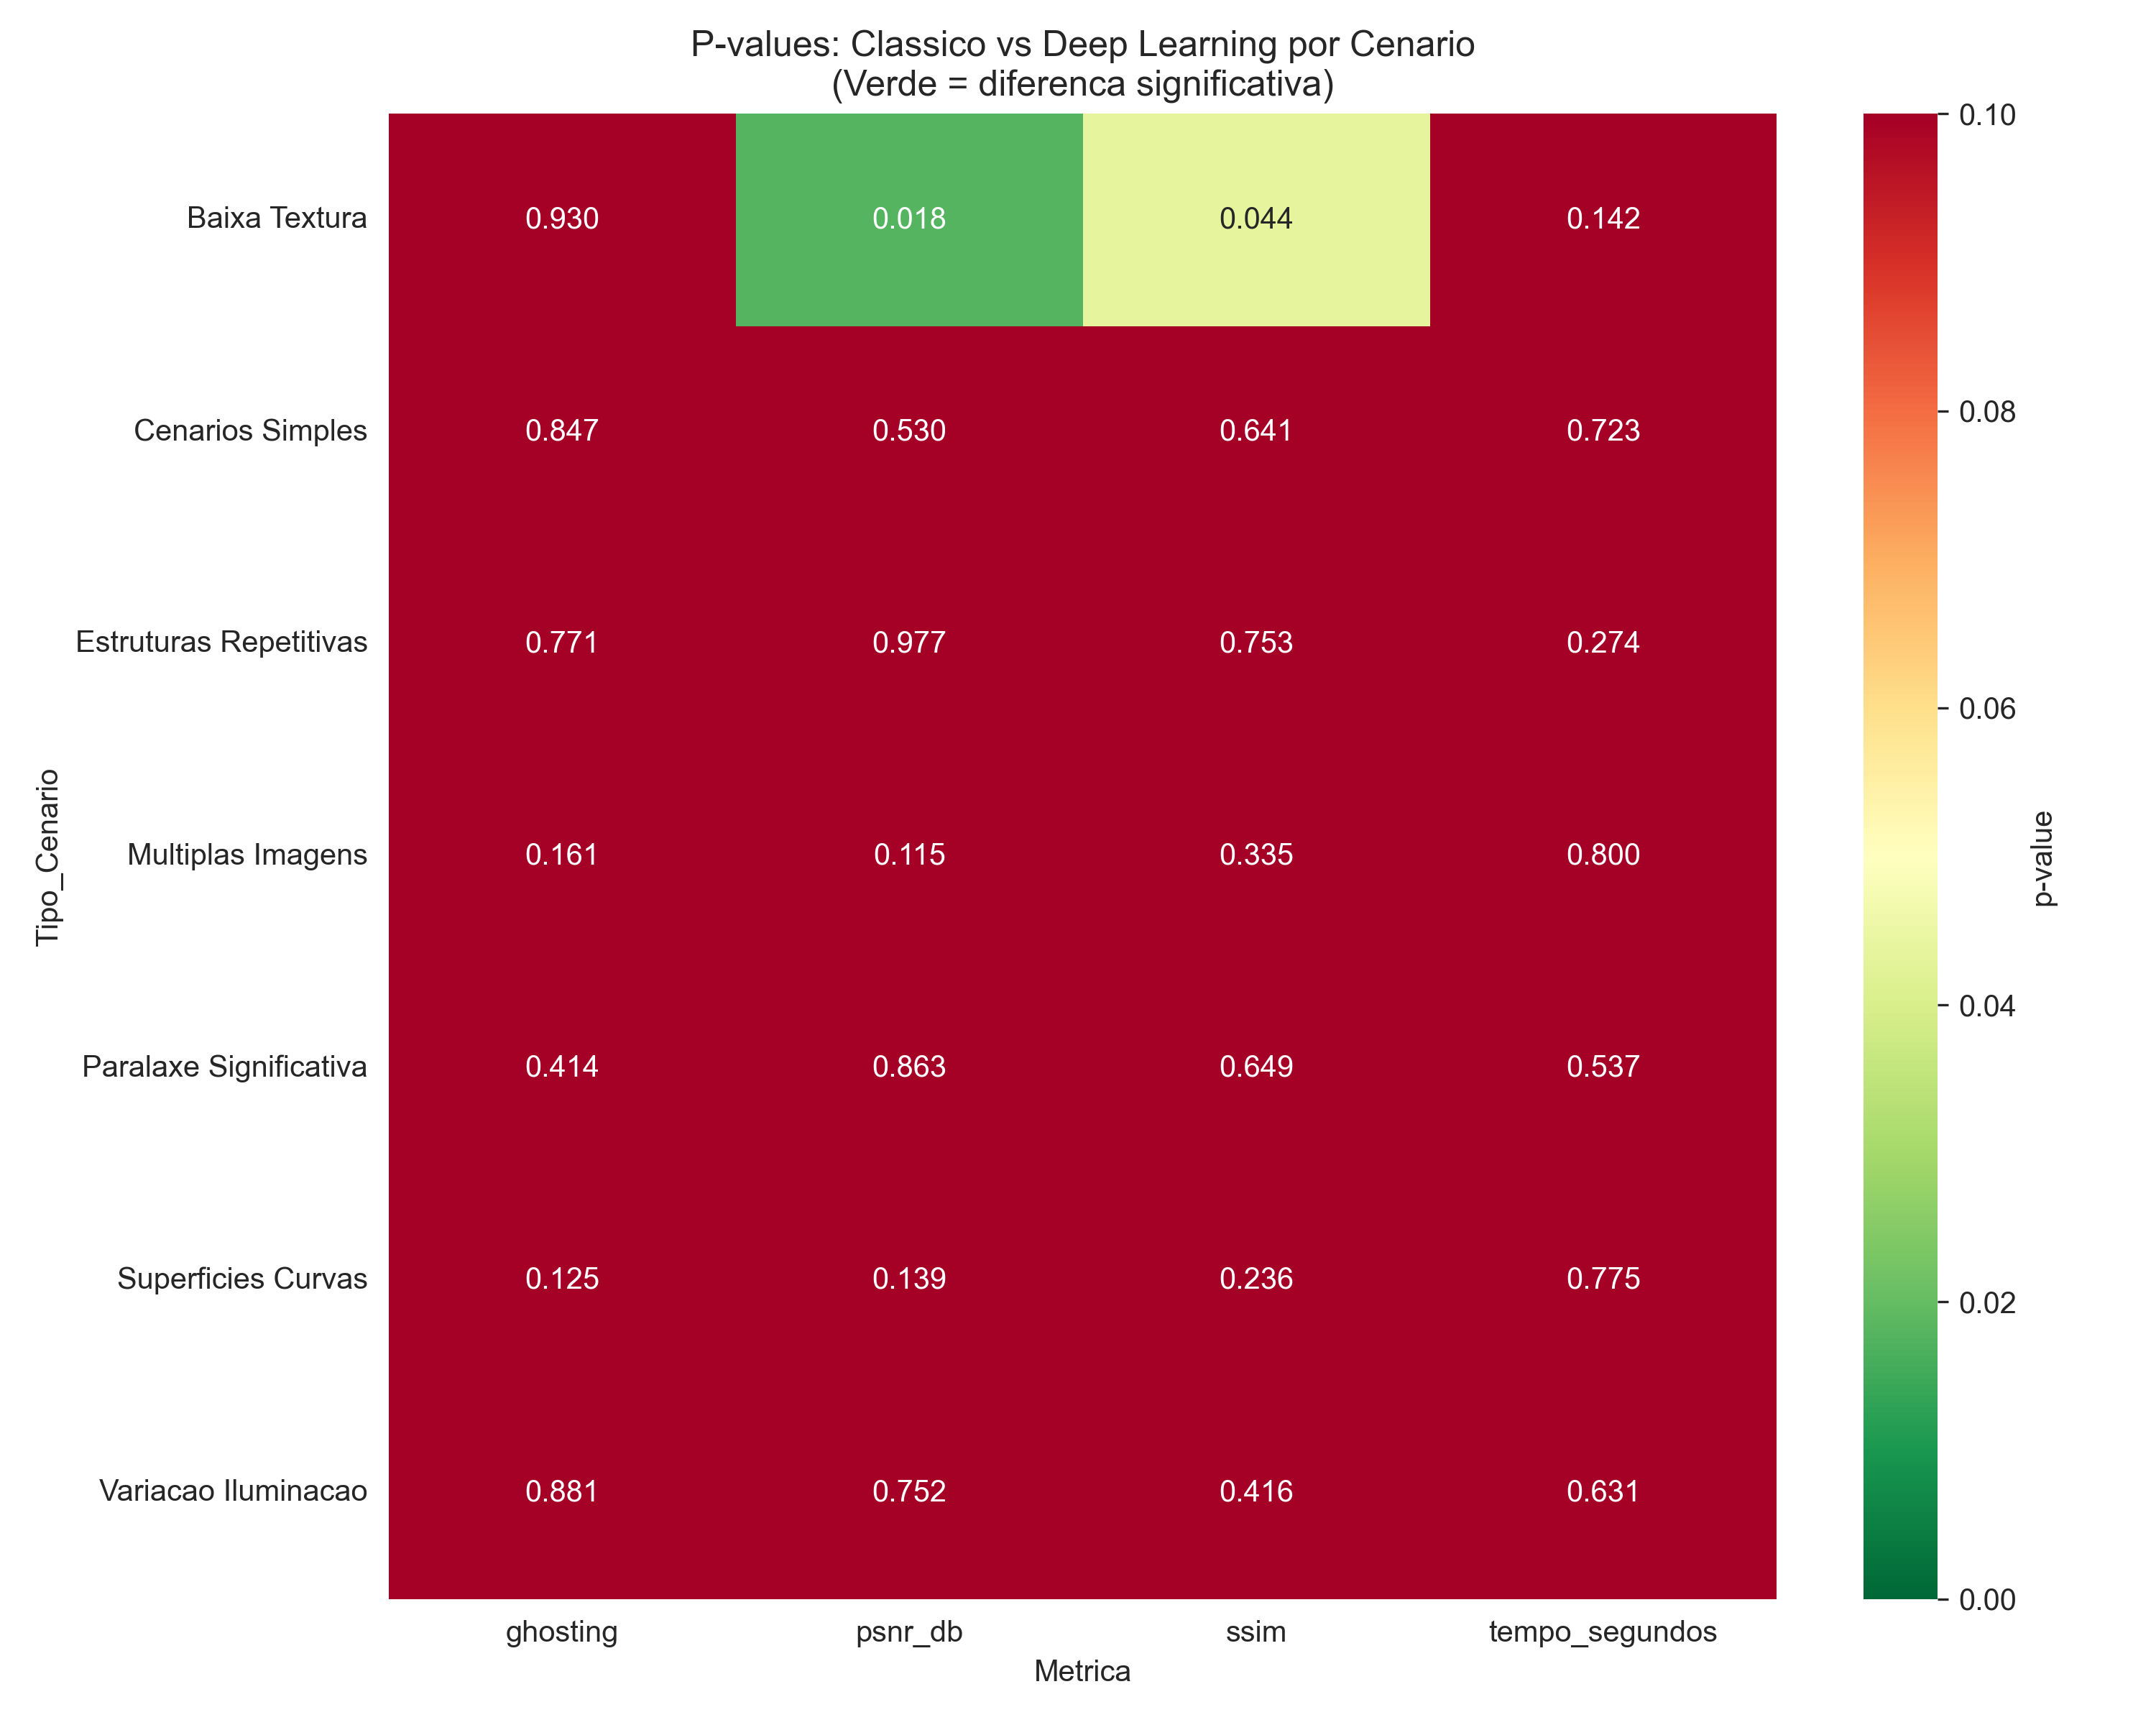
\includegraphics[width=0.75\textwidth]{figuras/resultados/heatmap_pvalues_por_cenario.png}
\caption{P-values dos testes Mann-Whitney U por tipo de cenário e métrica (verde = diferença significativa)}
\label{fig:heatmap_pvalues}
\fonte{Autoria própria (2025).}
\end{figure}

\subsection{Tamanho do Efeito por Cenário}

Complementando a análise de significância estatística, a Figura~\ref{fig:heatmap_cohens_d} apresenta o tamanho do efeito (Cohen's \textit{d}) para cada combinação de cenário e métrica, permitindo avaliar a magnitude prática das diferenças observadas.

\begin{figure}[htb]
\centering
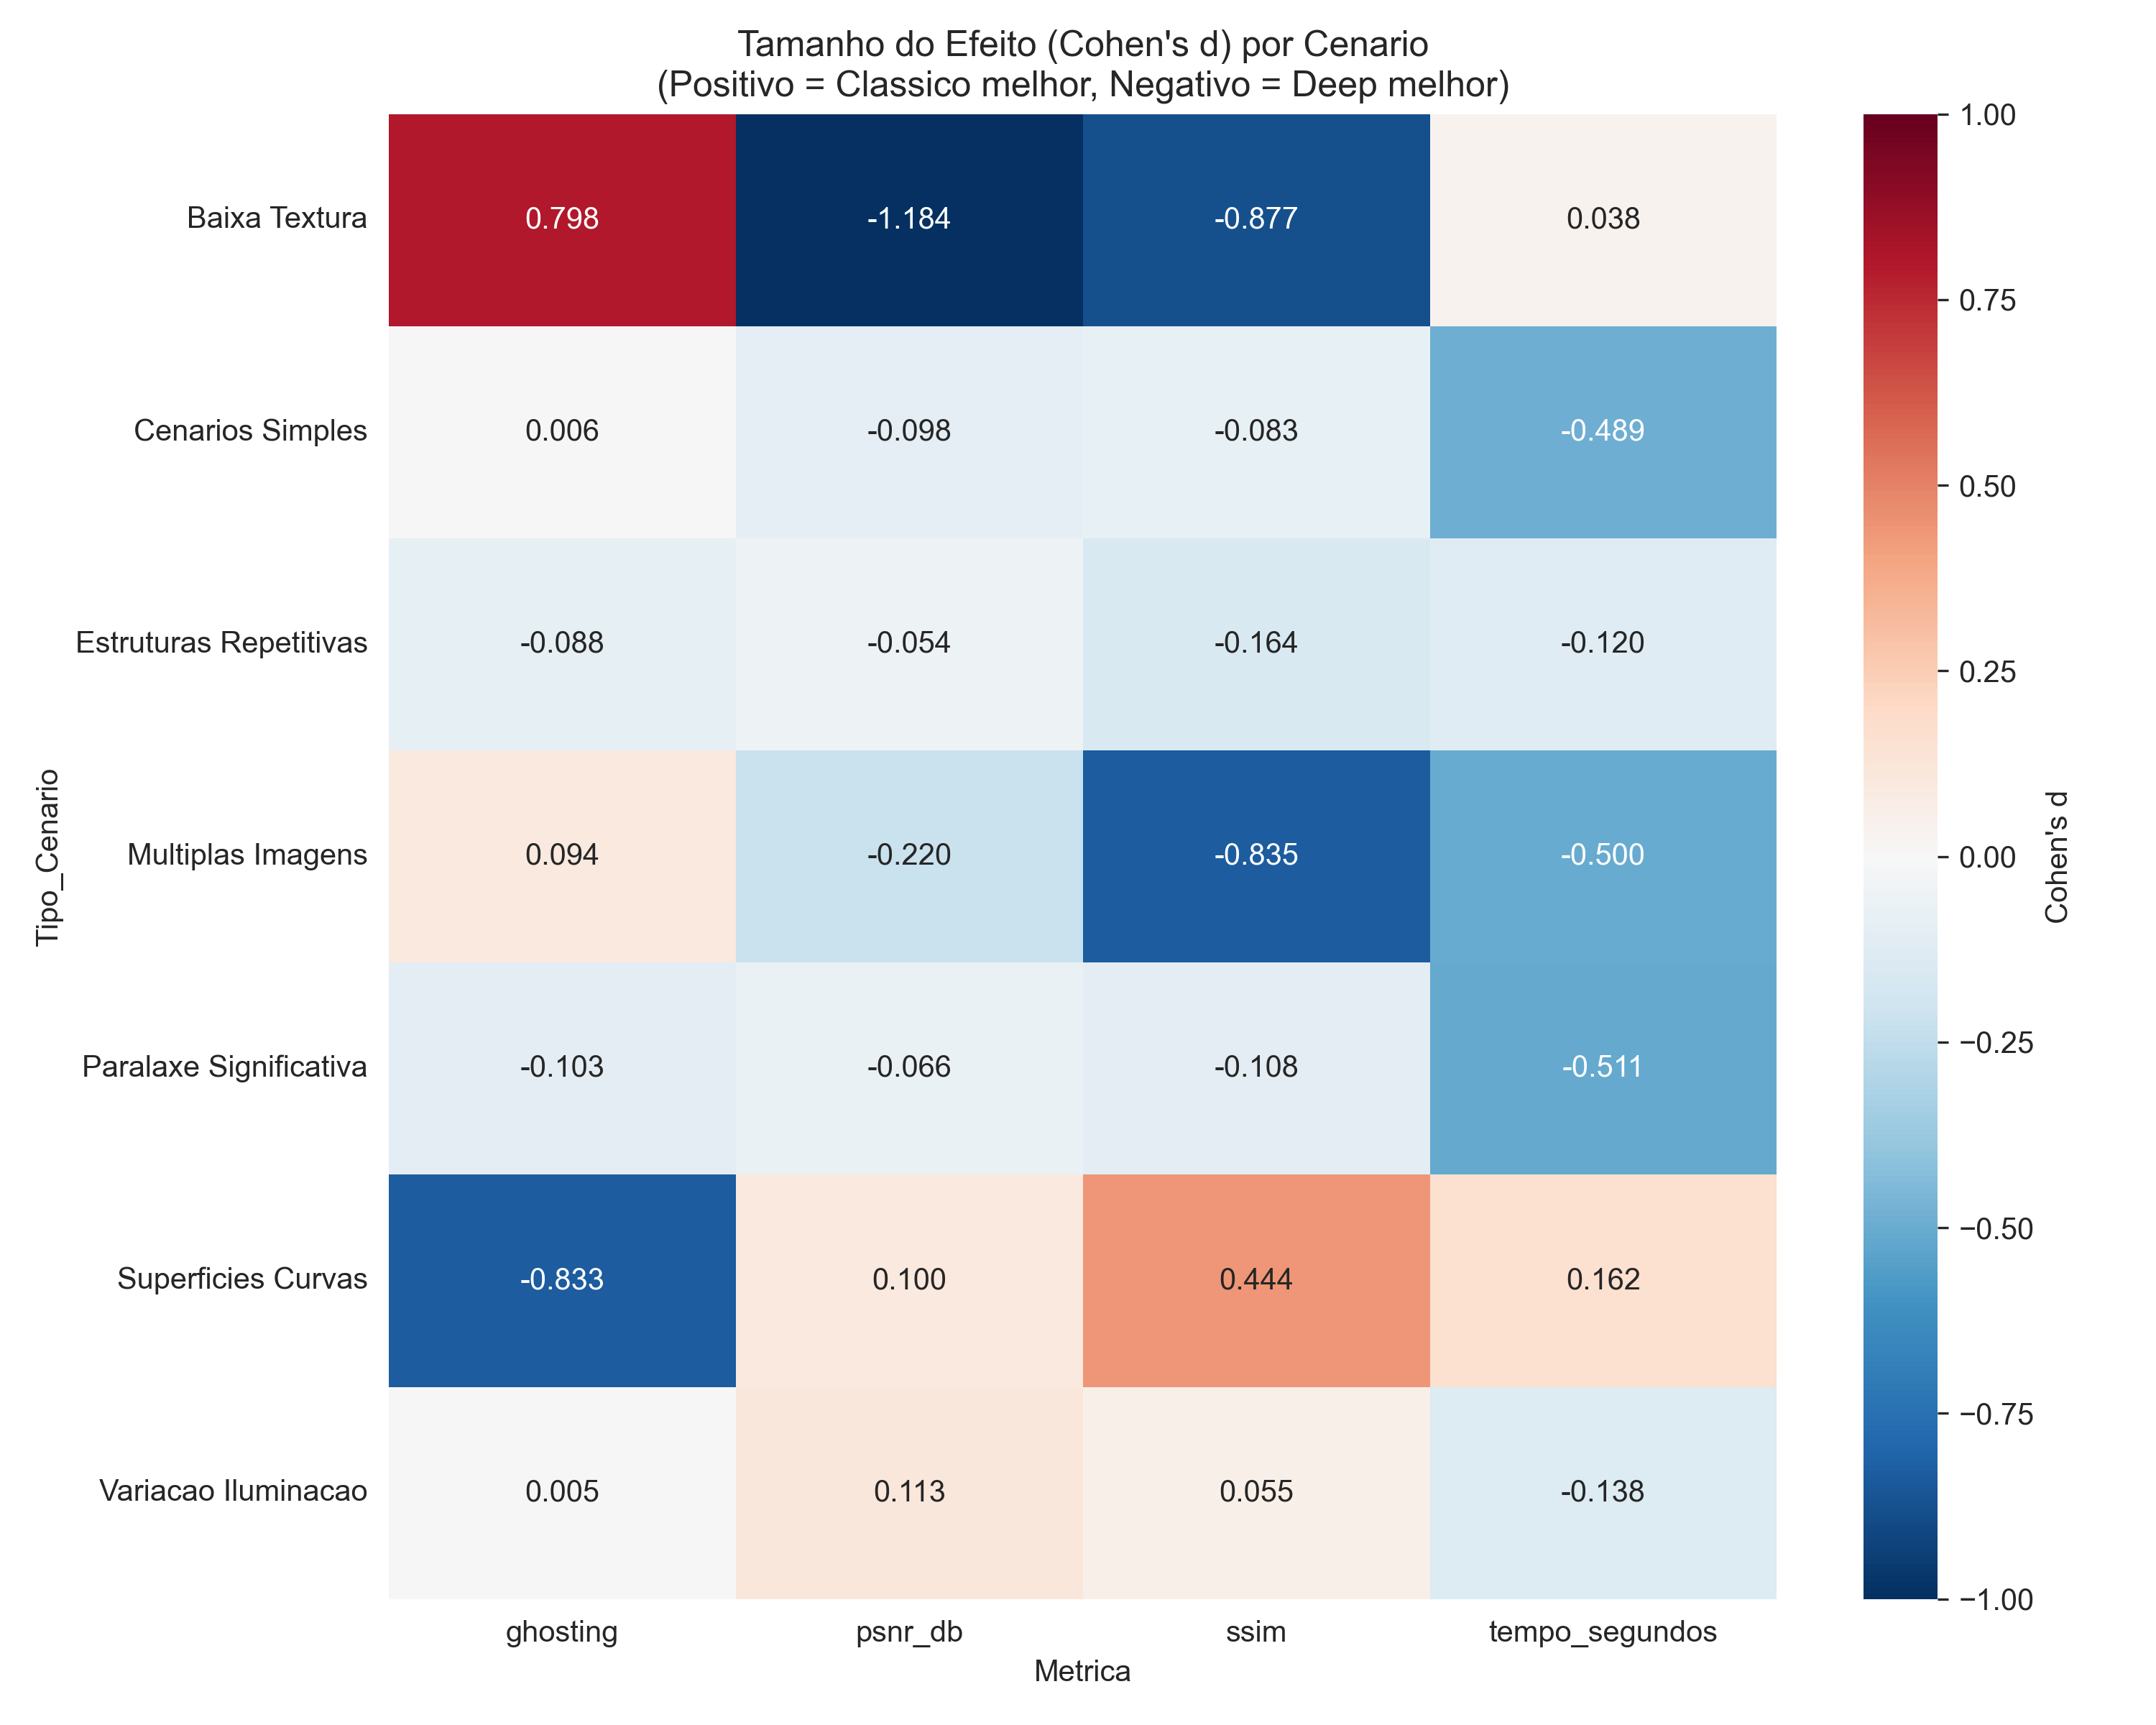
\includegraphics[width=0.75\textwidth]{figuras/resultados/heatmap_cohens_d_por_cenario.png}
\caption{Mapa de calor do tamanho do efeito (Cohen's d) por cenário e métrica. Valores próximos de zero indicam diferenças triviais.}
\label{fig:heatmap_cohens_d}
\fonte{Autoria própria (2025).}
\end{figure}

O mapa de calor confirma que, mesmo nos casos onde diferenças estatisticamente significativas foram detectadas (baixa textura), o tamanho do efeito permanece modesto. Na maioria dos cenários, Cohen's \textit{d} está próximo de zero, reforçando a equivalência prática entre as abordagens.

\subsection{Comparação Visual por Cenário}

A Figura~\ref{fig:barplot_cenarios} apresenta comparação visual das métricas principais por tipo de cenário, facilitando a identificação de padrões de desempenho.

\begin{figure}[htb]
\centering
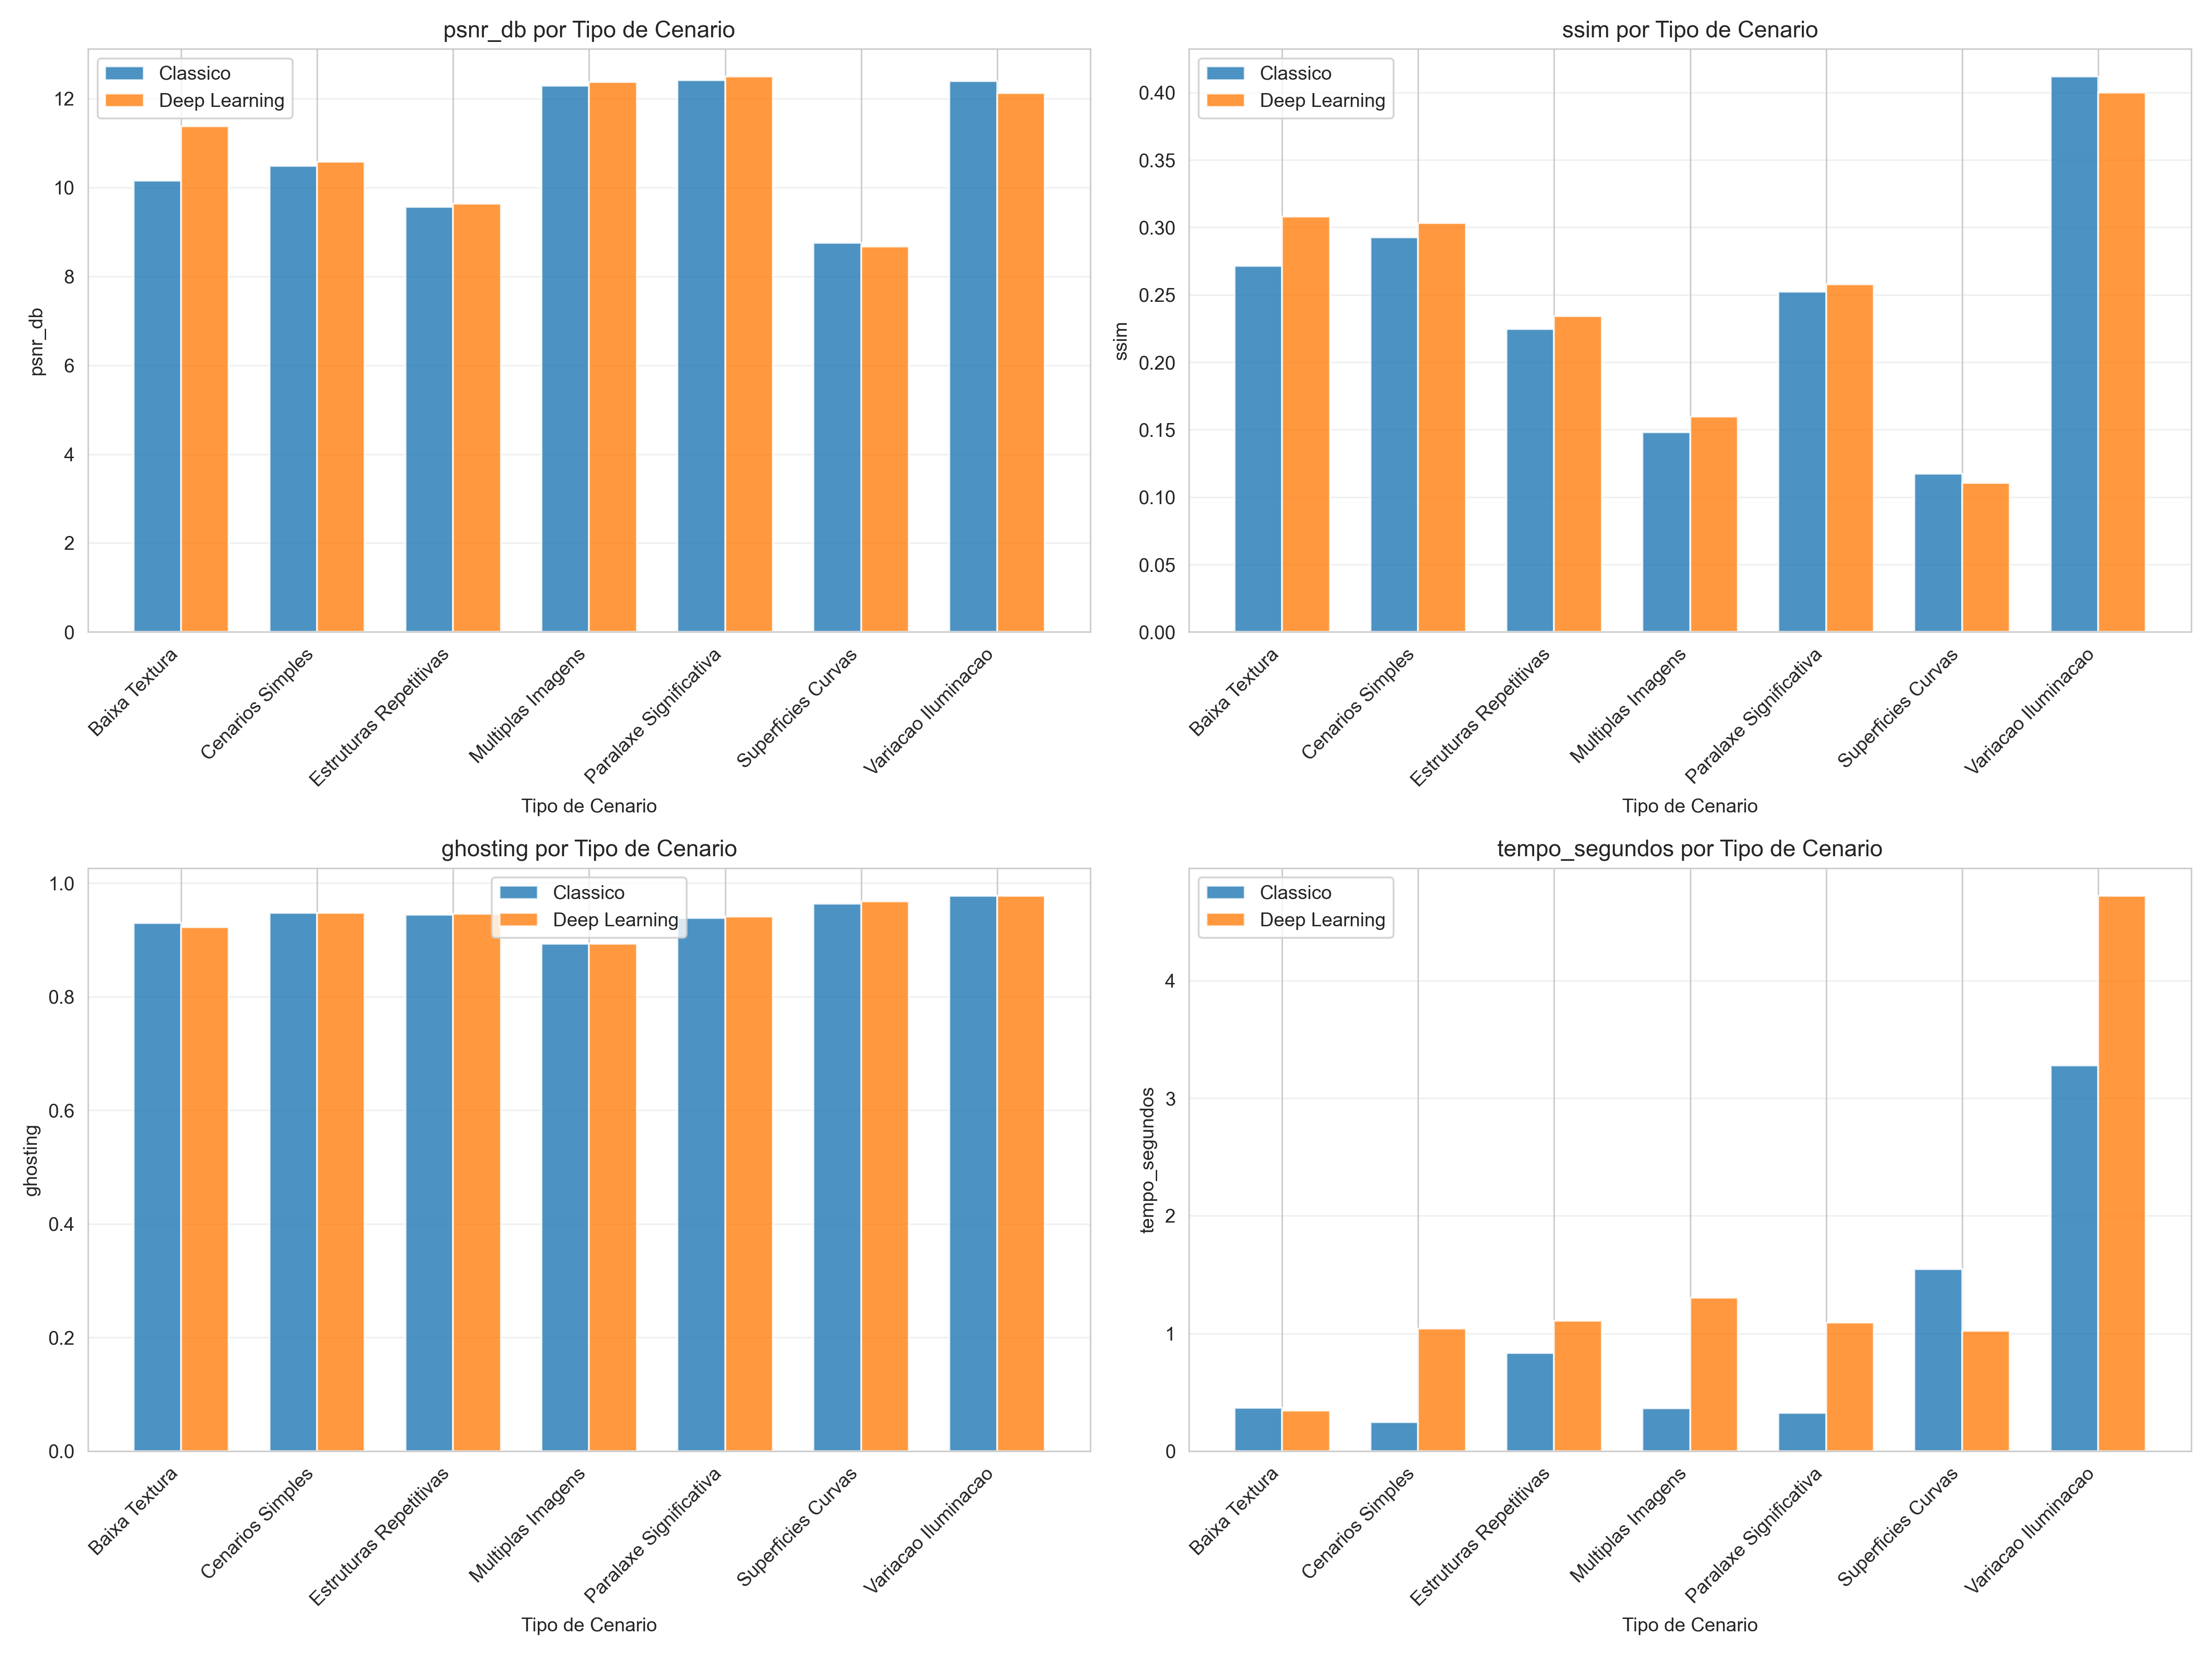
\includegraphics[width=\textwidth]{figuras/resultados/barplot_metricas_por_cenario.png}
\caption{Comparação das métricas PSNR e SSIM por tipo de cenário (Clássico vs Deep Learning)}
\label{fig:barplot_cenarios}
\fonte{Autoria própria (2025).}
\end{figure}

\subsection{Trade-off Qualidade vs Velocidade por Cenário}

A Figura~\ref{fig:scatter_psnr_tempo_cenario} apresenta a relação entre qualidade (PSNR) e tempo de processamento, estratificada por tipo de cenário, revelando que o trade-off varia conforme as características do dataset.

\begin{figure}[htb]
\centering
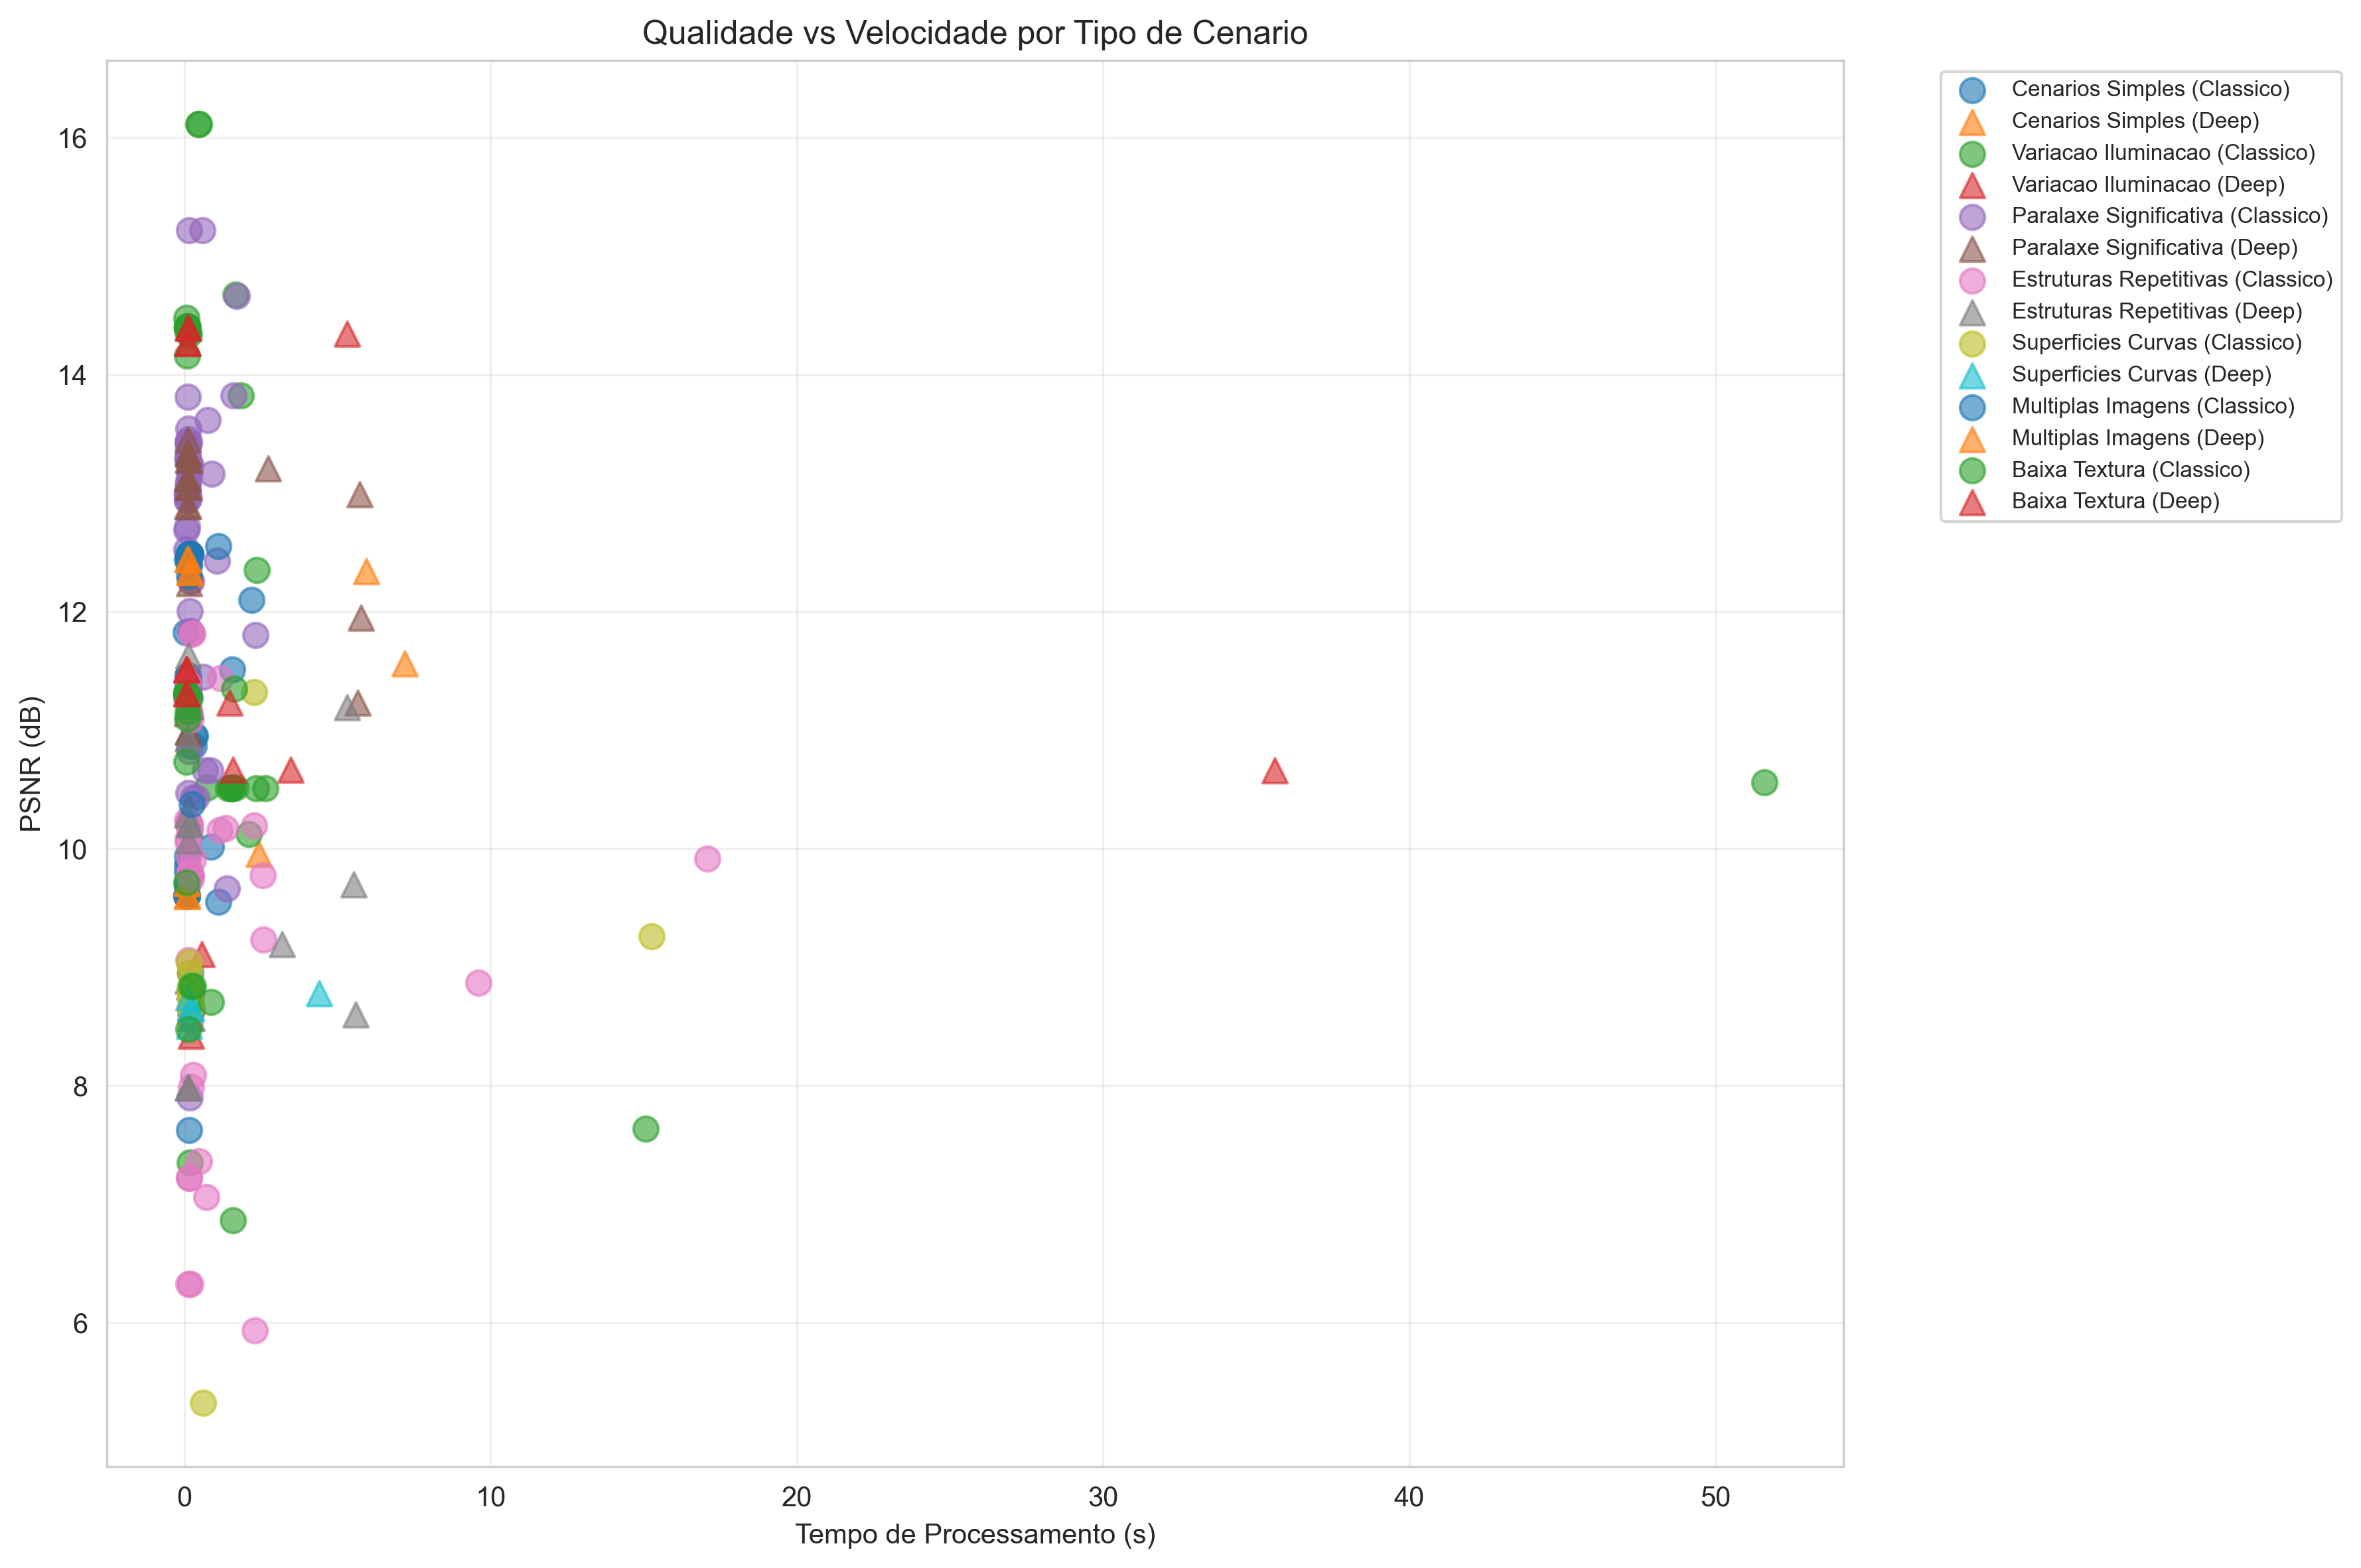
\includegraphics[width=0.9\textwidth]{figuras/resultados/scatter_psnr_tempo_por_cenario.png}
\caption{Scatter plot: PSNR vs Tempo de processamento por tipo de cenário}
\label{fig:scatter_psnr_tempo_cenario}
\fonte{Autoria própria (2025).}
\end{figure}

Observa-se que cenários de baixa textura e múltiplas imagens tendem a exigir maior tempo de processamento, enquanto cenários simples permitem processamento mais rápido sem comprometer significativamente a qualidade.

\section{Análise de Casos Extremos}

A análise de casos extremos permite identificar padrões nas condições que levam ao sucesso ou falha de diferentes métodos de fusão. Esta seção examina os melhores e piores resultados obtidos, revelando características importantes para seleção apropriada de técnicas.

\subsection{Datasets Mais Desafiadores}

Os cinco conjuntos de imagens que apresentaram maior dificuldade para todos os métodos testados foram:

\begin{enumerate}
    \item \texttt{no\_contractor\_parking\_1}: PSNR médio de 8,51 dB
    \item \texttt{graffiti\_car\_1}: PSNR médio de 8,73 dB
    \item \texttt{rental\_office\_1}: PSNR médio de 9,01 dB
    \item \texttt{stop\_sign\_1}: PSNR médio de 9,74 dB
    \item \texttt{theory\_left}: PSNR médio de 9,86 dB
\end{enumerate}

Estes datasets compartilham características que tornam a fusão particularmente desafiadora: baixo contraste, estruturas altamente repetitivas ou paralaxe pronunciada. A análise detalhada destes casos revela limitações fundamentais das abordagens baseadas em homografia planar global, que assumem transformação perspectiva única entre as imagens.

Em cenários com paralaxe significativa, onde objetos em diferentes profundidades sofrem deslocamentos relativos distintos, nenhuma transformação global consegue alinhar perfeitamente todas as regiões simultaneamente. Isto resulta em artefatos visíveis nas regiões de sobreposição, manifestando-se como ghosting ou distorções geométricas.

\subsection{Padrões de Sucesso e Falha}

Definindo sucesso como PSNR $\geq 12{,}48$ dB (quartil superior) e falha como PSNR $\leq 9{,}71$ dB (quartil inferior), foram identificados 76 casos de sucesso e 75 casos de falha.

\textbf{Métodos com maior taxa de sucesso:}
\begin{itemize}
    \item Clássico • Blend Hybrid: 5 casos
    \item Clássico • Blend Laplacian: 5 casos
    \item Clássico • Blend Exposure: 5 casos
\end{itemize}

\textbf{Métodos com maior taxa de falha:}
\begin{itemize}
    \item Clássico • Blend Poisson: 11 casos
    \item Clássico • Ecc Alignment: 6 casos
    \item Deep • Flow Stitch: 5 casos
\end{itemize}

Observa-se que métodos que combinam múltiplas técnicas avançadas (compensação de exposição, pirâmides Laplacianas, mesclagem multiescala) tendem a apresentar maior robustez, enquanto métodos mais simples ou especializados (Poisson blending, alinhamento ECC, flow-based stitching) são mais susceptíveis a falhas em cenários desafiadores.

A Figura~\ref{fig:violin_extremos} apresenta a distribuição de PSNR por dataset, comparando métodos clássicos e deep learning.

\begin{figure}[htb]
\centering
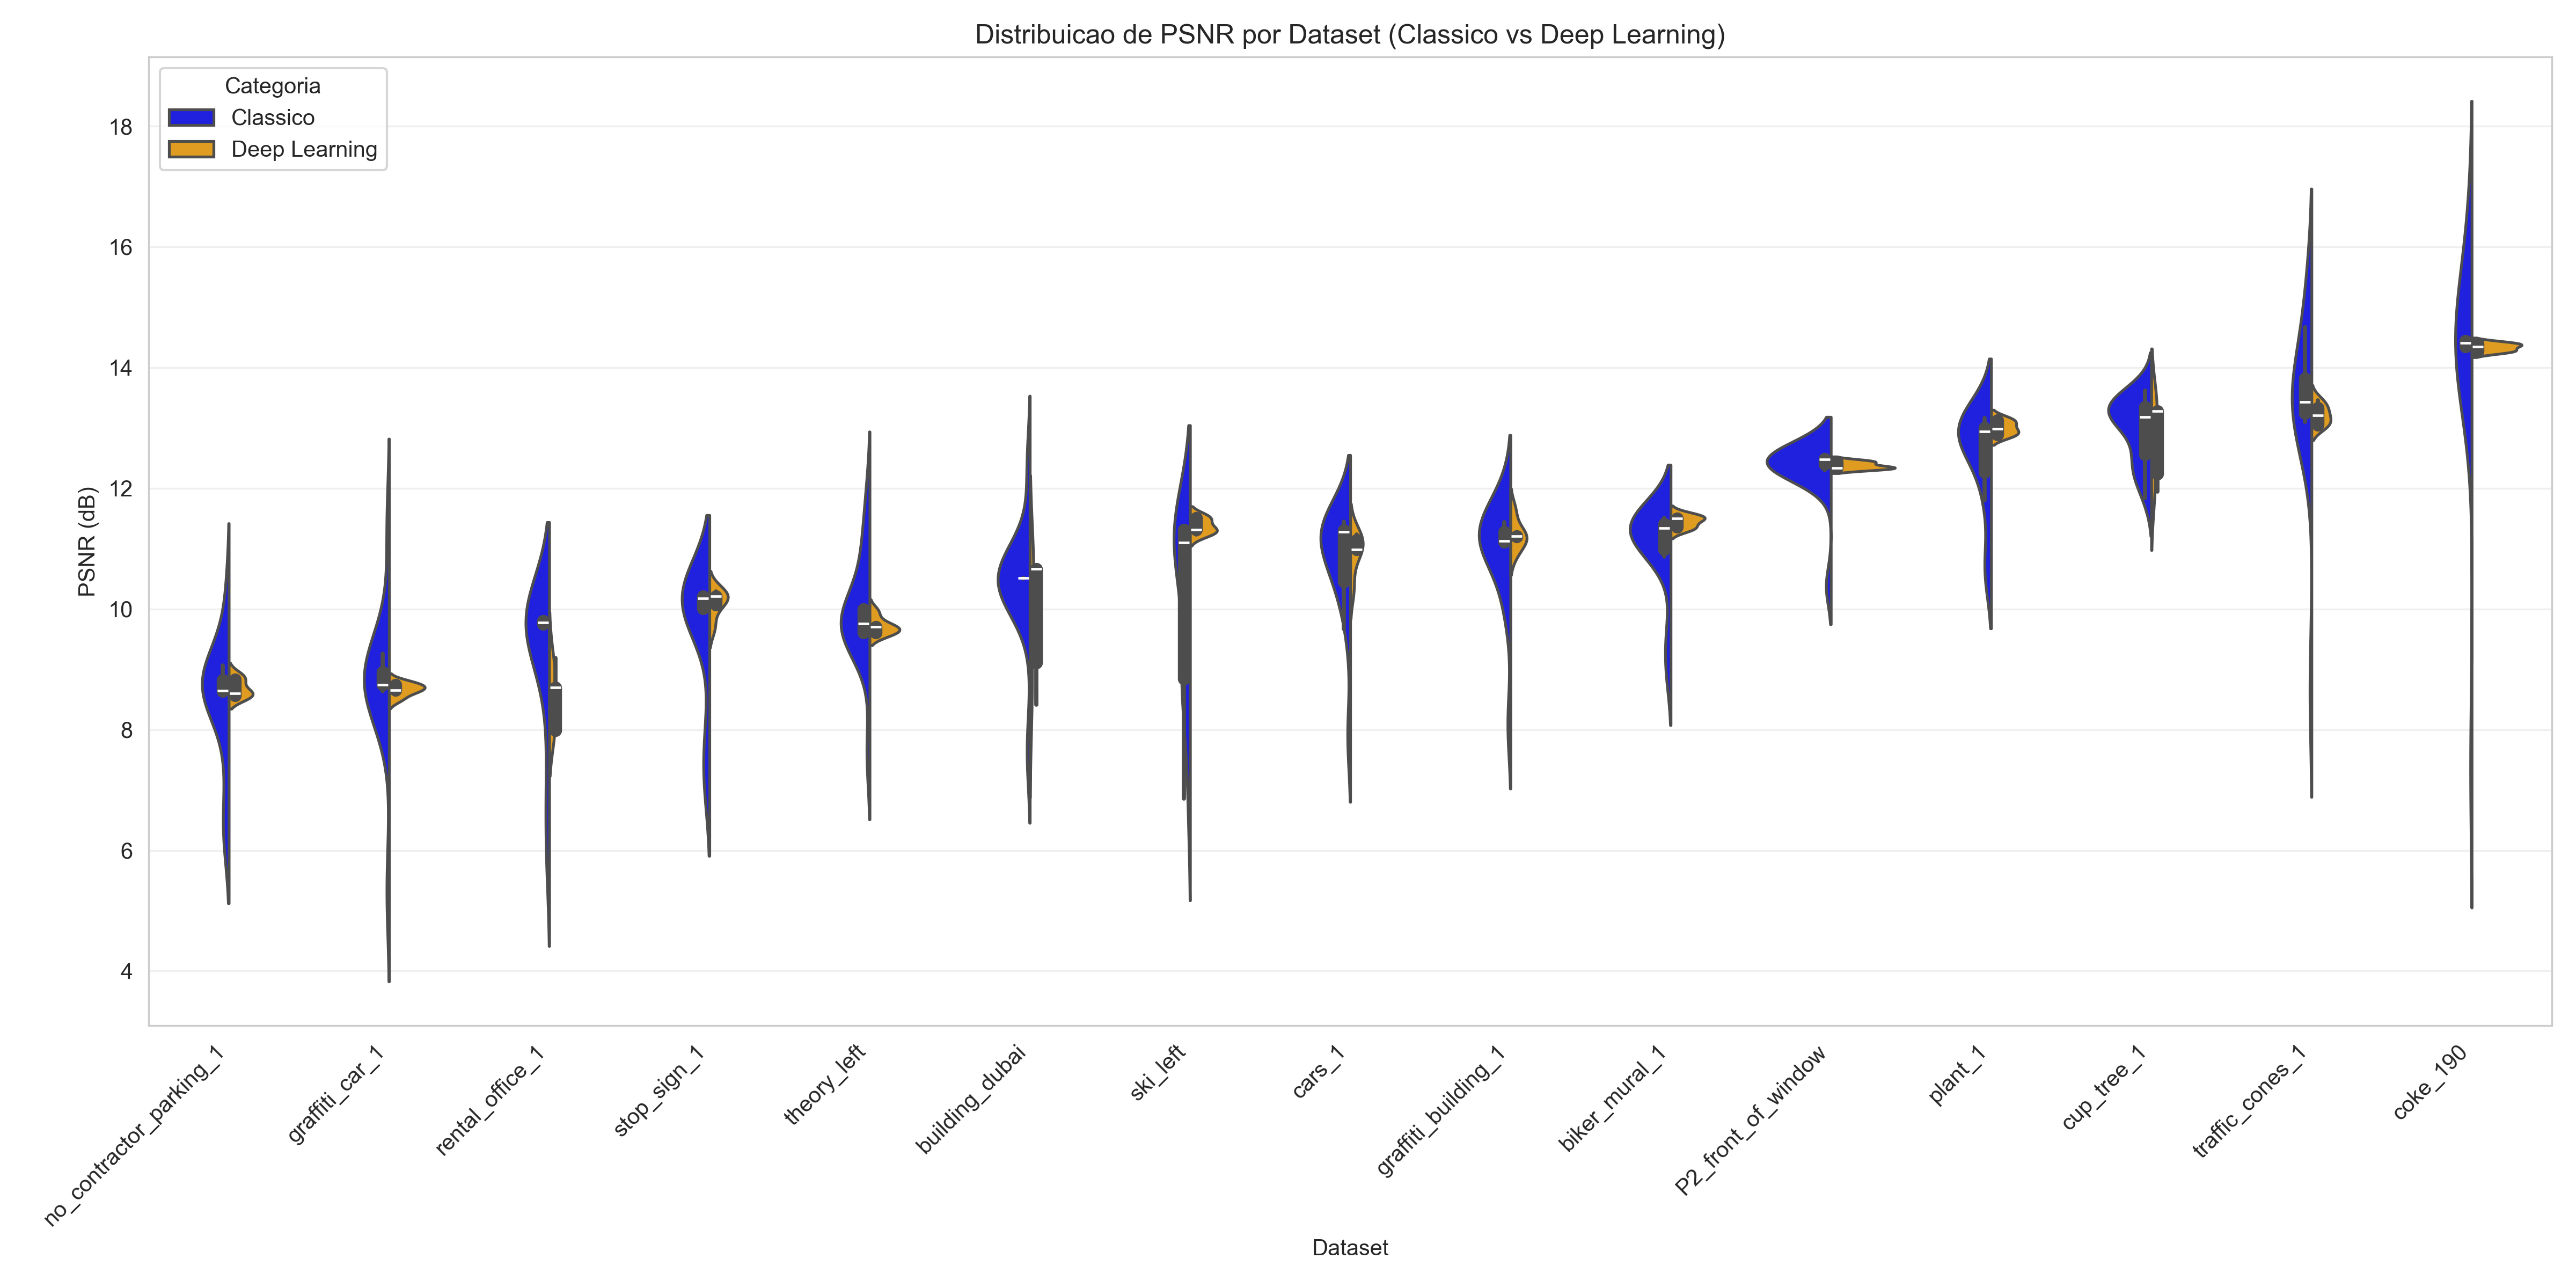
\includegraphics[width=\textwidth]{figuras/resultados/violin_psnr_por_dataset.png}
\caption{Distribuição de PSNR por dataset: Clássico vs Deep Learning (violin plots)}
\label{fig:violin_extremos}
\fonte{Autoria própria (2025).}
\end{figure}

Os violin plots revelam que a variabilidade de desempenho é altamente dependente do dataset específico, com alguns conjuntos apresentando distribuições amplas (indicando alta sensibilidade à escolha do método) e outros apresentando distribuições estreitas (indicando resultados consistentes independentemente do método).

\subsection{Distribuição de Sucesso e Falha}

A Figura~\ref{fig:distribuicao_extremos} apresenta a distribuição dos casos de sucesso (PSNR alto) e falha (PSNR baixo) por categoria de método.

\begin{figure}[htb]
\centering
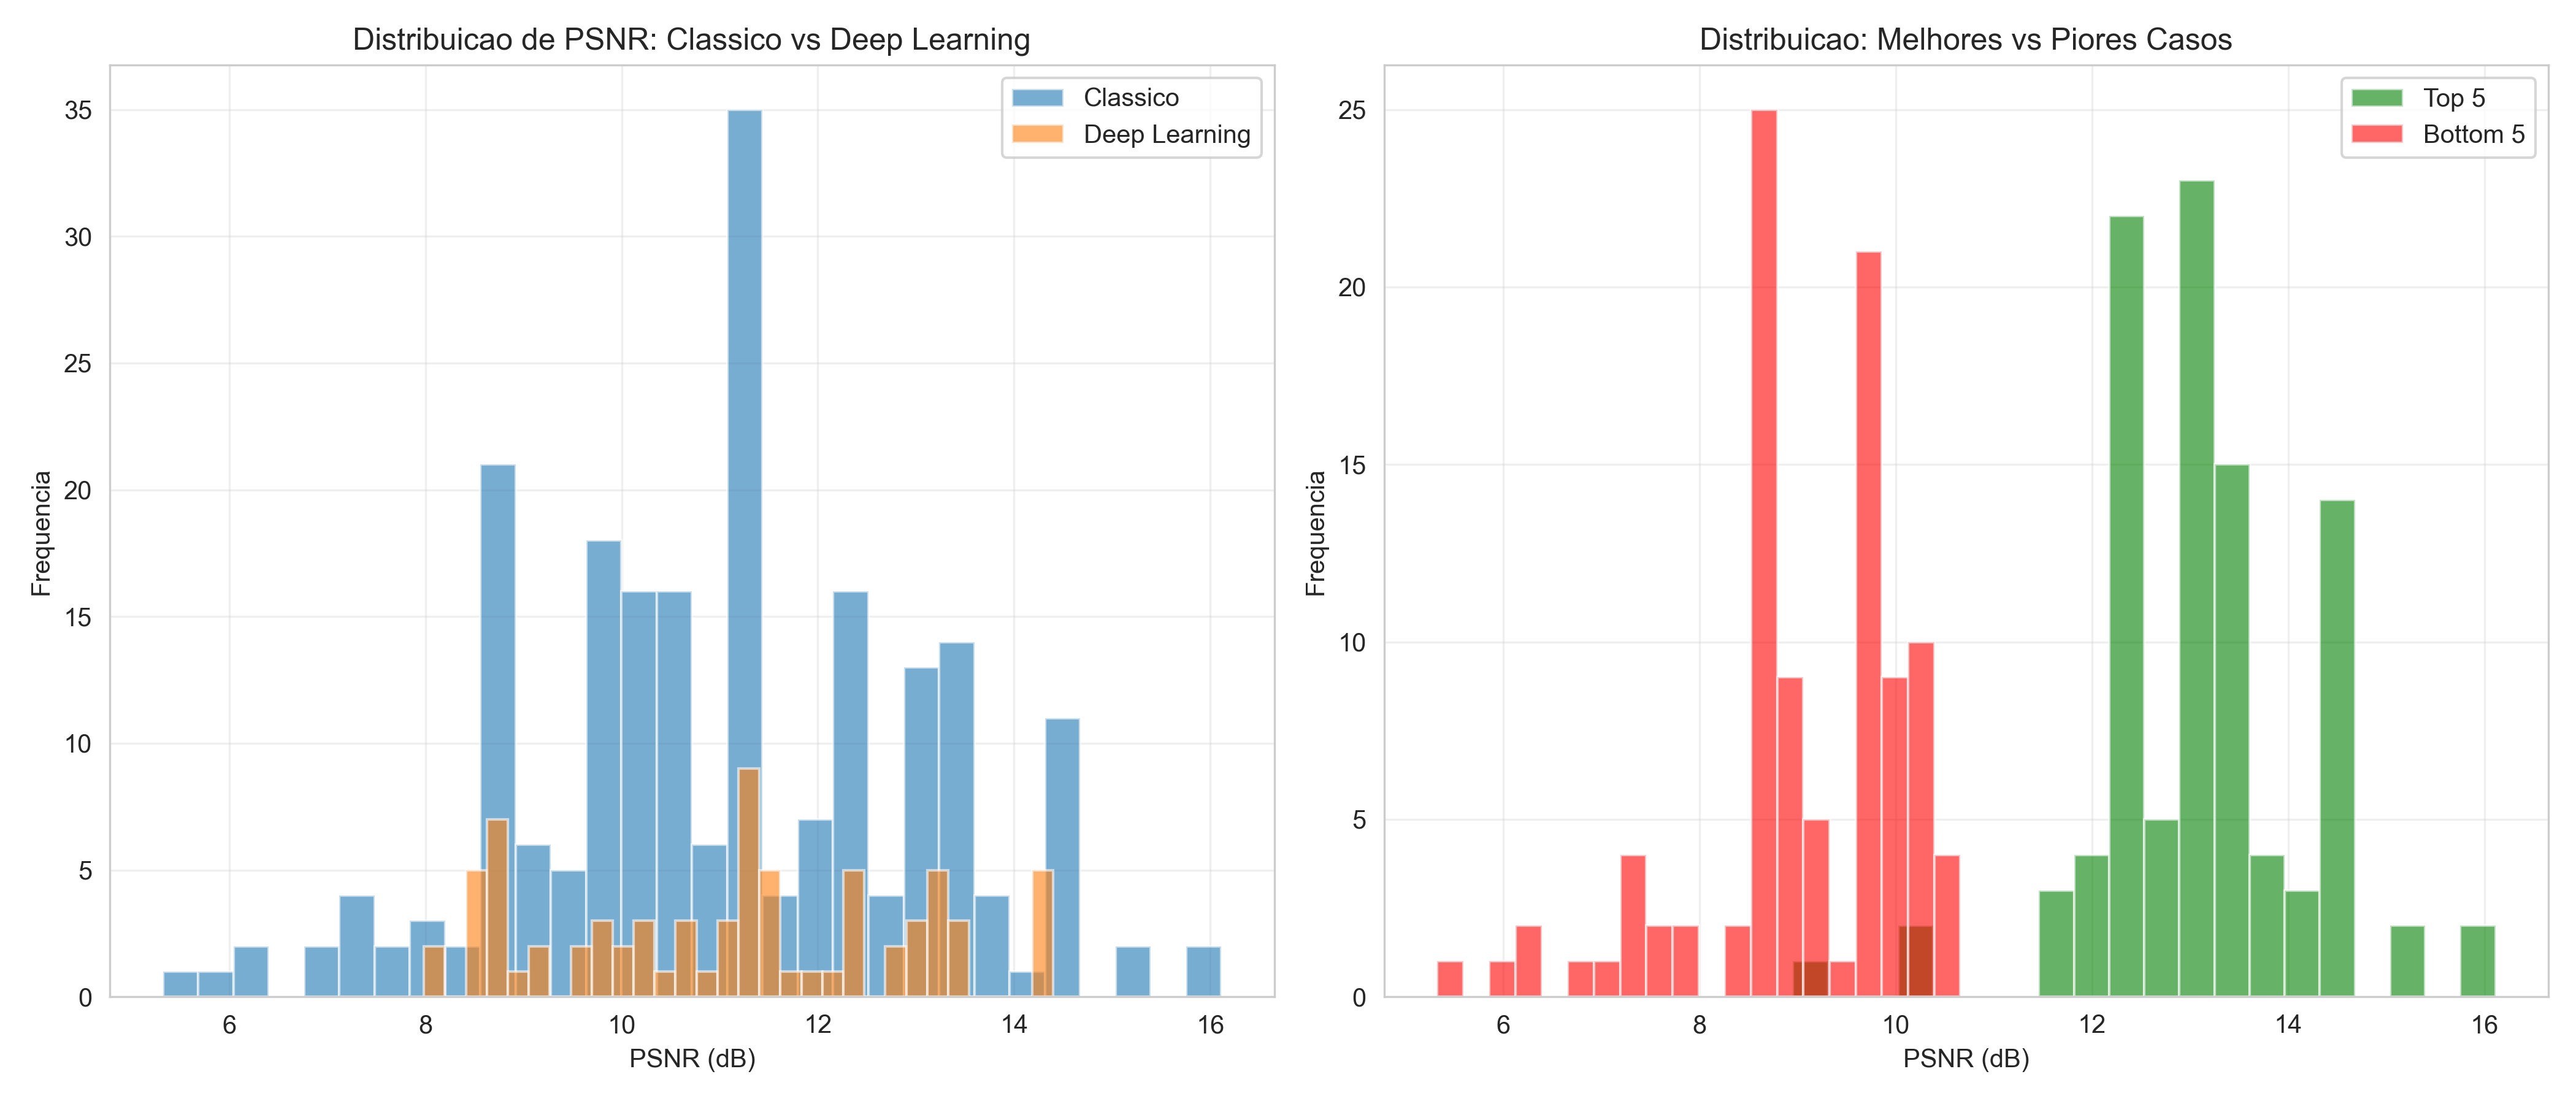
\includegraphics[width=0.8\textwidth]{figuras/resultados/distribuicao_casos_extremos.png}
\caption{Distribuição de casos extremos: sucessos e falhas por categoria}
\label{fig:distribuicao_extremos}
\fonte{Autoria própria (2025).}
\end{figure}

Ambas as categorias apresentam distribuição similar de sucessos e falhas, confirmando equivalência de robustez entre métodos clássicos e deep learning.

\subsection{Variabilidade de Desempenho por Método}

A Figura~\ref{fig:boxplot_range_metodo} apresenta a variabilidade (range) de PSNR para cada método, identificando aqueles com desempenho mais consistente versus aqueles mais sensíveis às características do dataset.

\begin{figure}[htb]
\centering
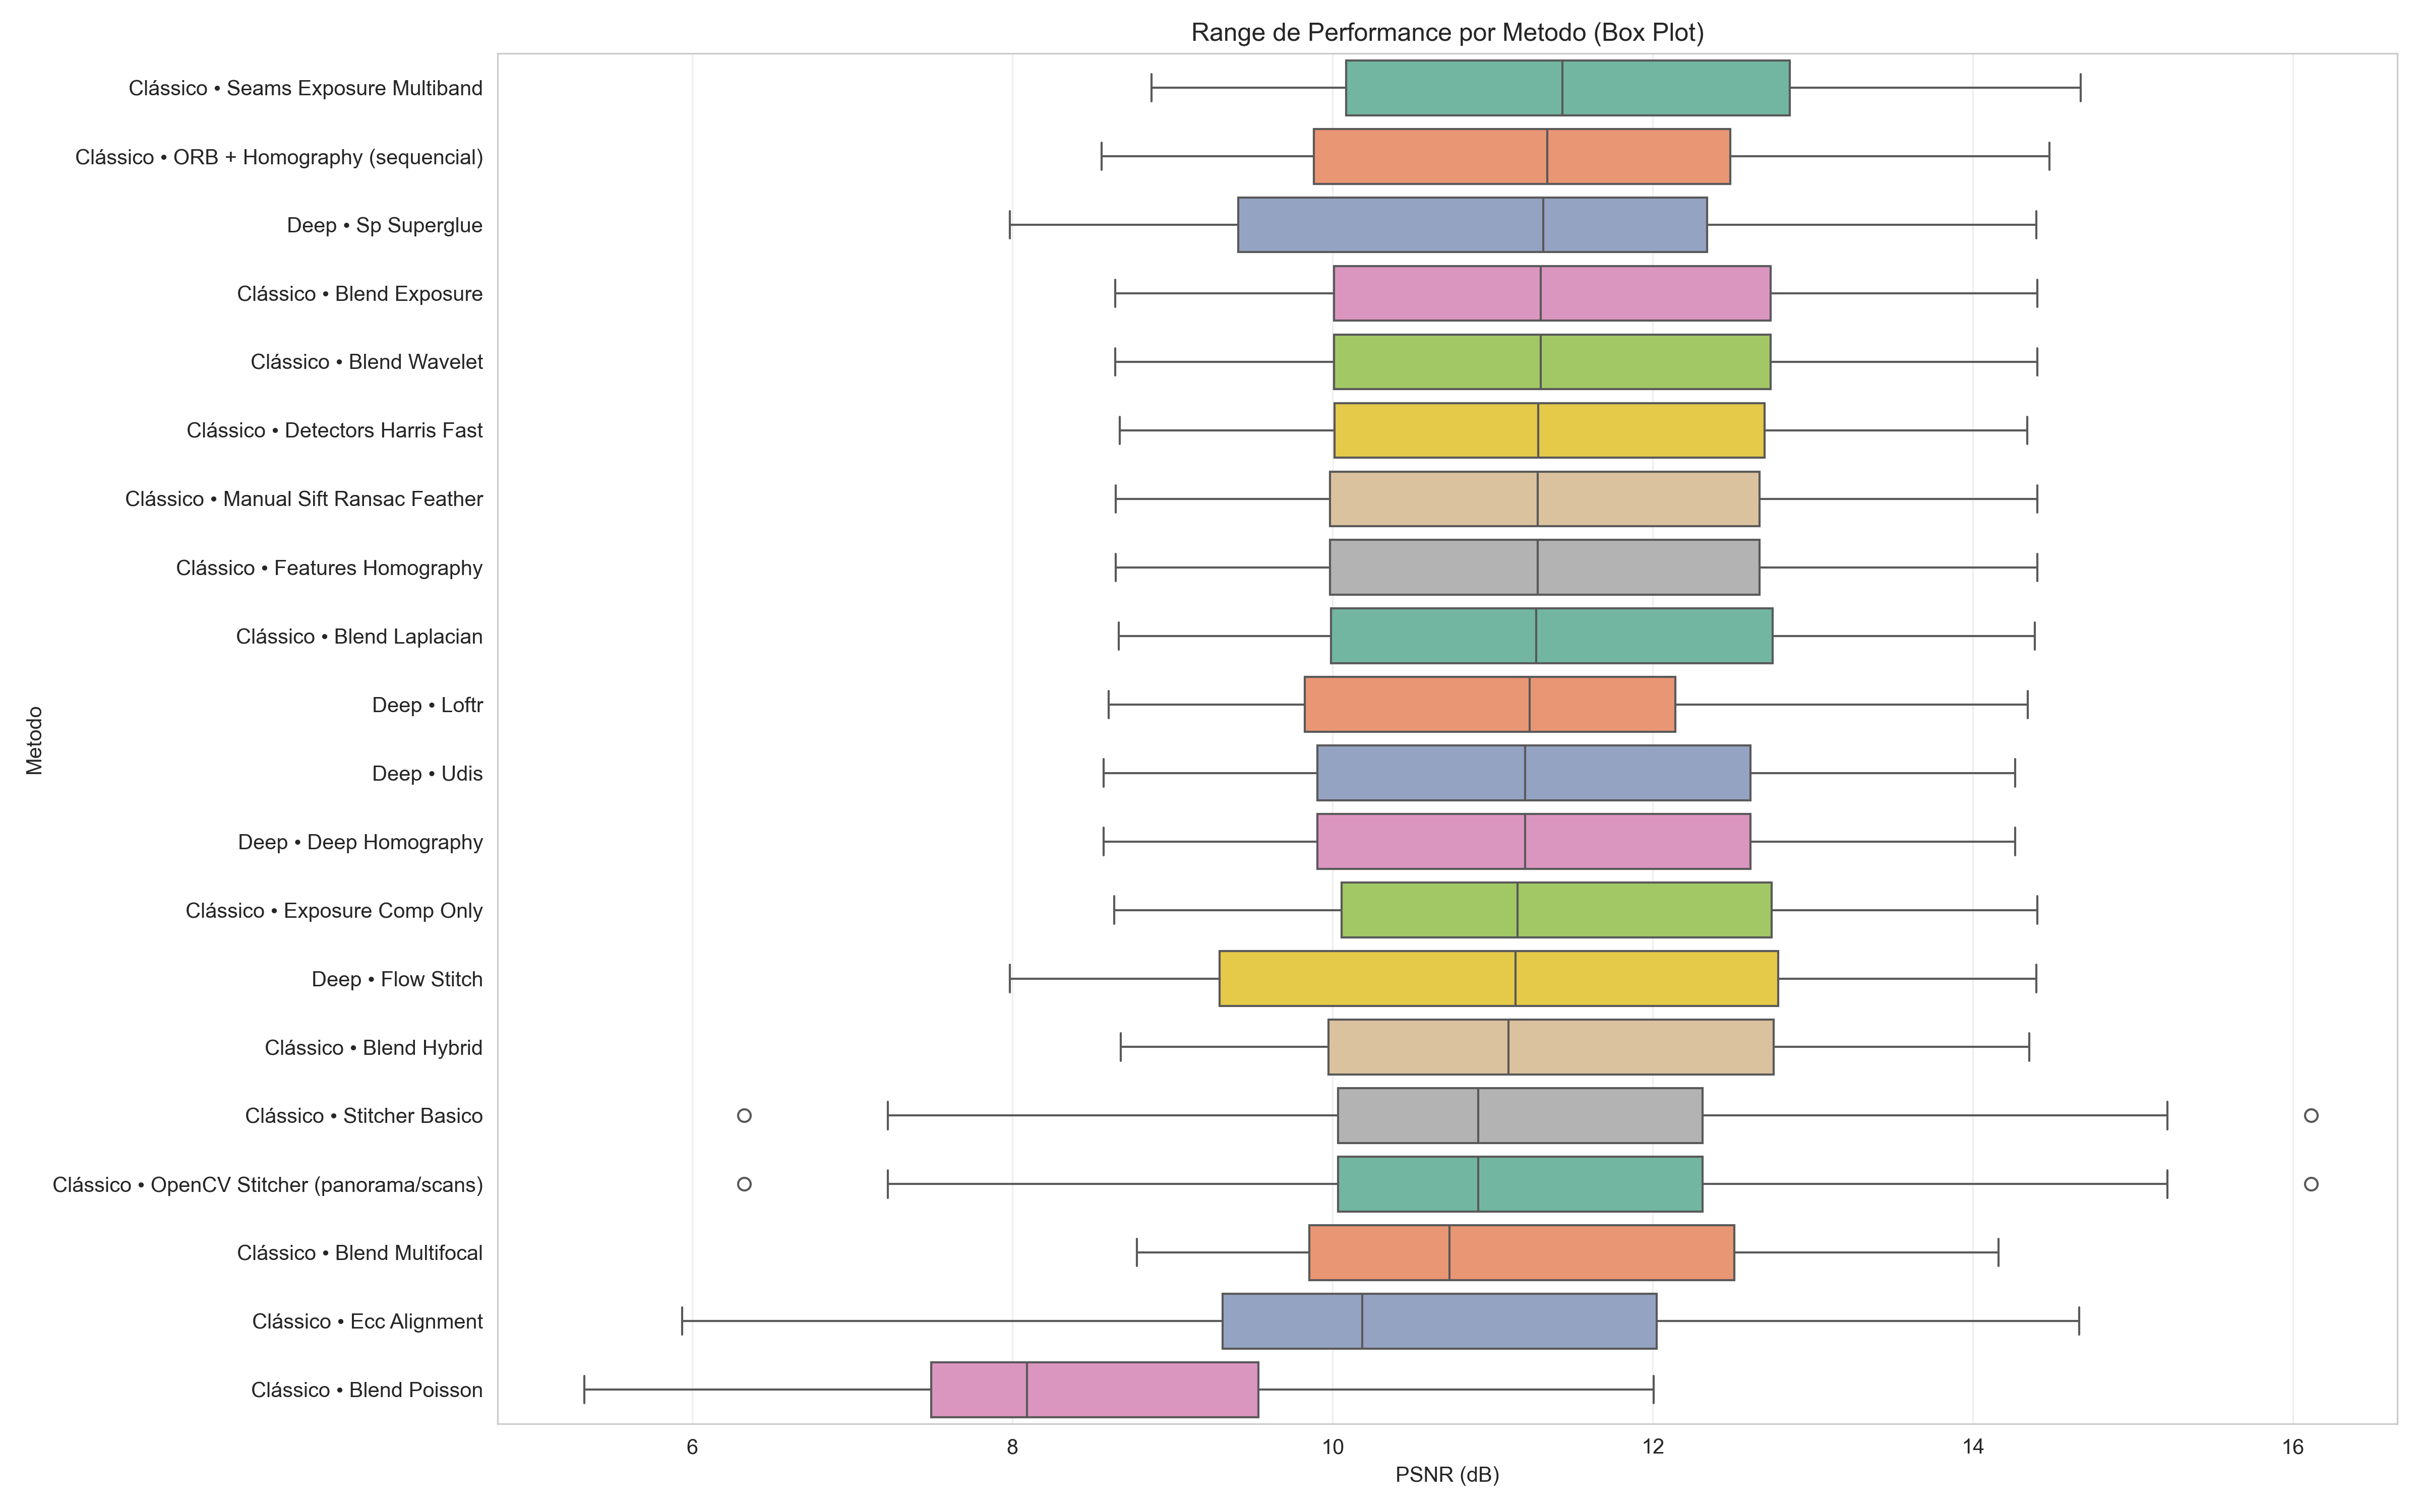
\includegraphics[width=\textwidth]{figuras/resultados/boxplot_range_por_metodo.png}
\caption{Box plots: variabilidade de PSNR por método. Boxes mais estreitos indicam maior consistência.}
\label{fig:boxplot_range_metodo}
\fonte{Autoria própria (2025).}
\end{figure}

Métodos como OpenCV Stitcher e Stitcher Basico apresentam menor variabilidade, indicando desempenho mais previsível e consistente através dos diferentes datasets.

\subsection{Melhores Métodos por Dataset}

A Figura~\ref{fig:heatmap_melhor_metodo} identifica qual método obteve melhor desempenho em cada dataset, revelando que não há vencedor universal -- a escolha ótima depende das características específicas de cada cenário.

\begin{figure}[htb]
\centering
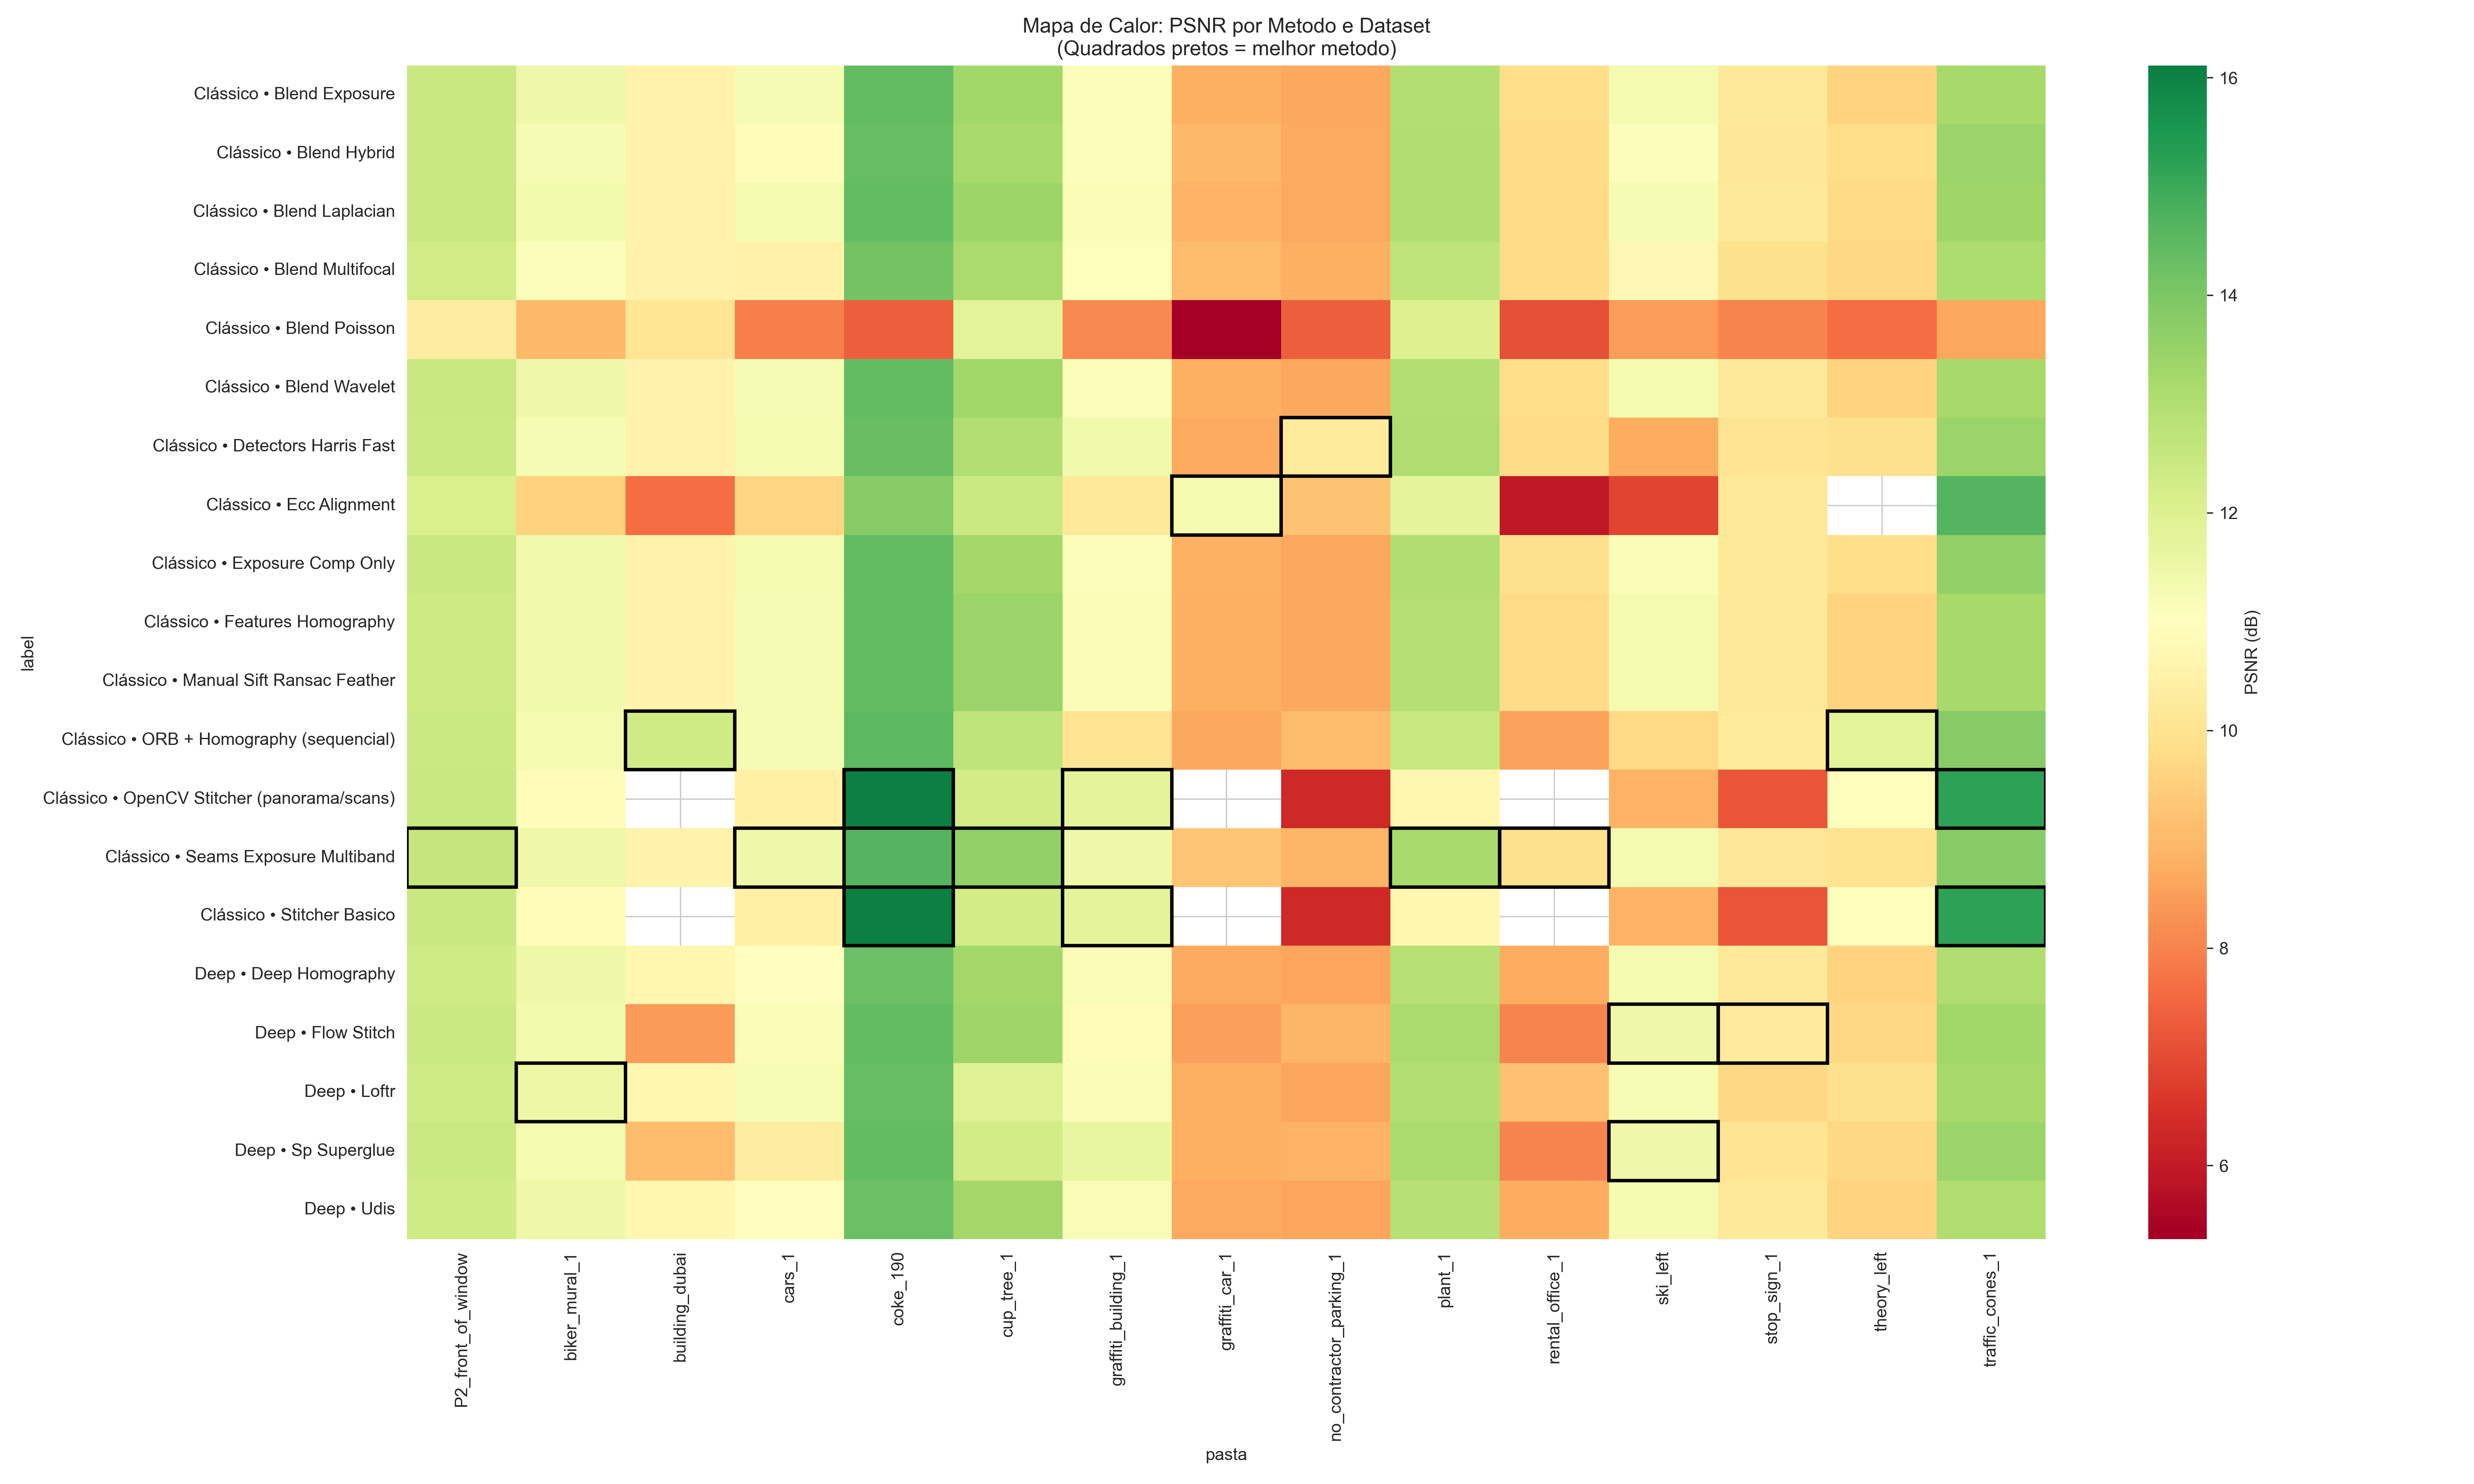
\includegraphics[width=\textwidth]{figuras/resultados/heatmap_melhor_metodo_por_dataset.png}
\caption{Mapa de identificação do melhor método por dataset e categoria}
\label{fig:heatmap_melhor_metodo}
\fonte{Autoria própria (2025).}
\end{figure}

\subsection{Ausência de Superioridade Absoluta}

Uma constatação importante é a \textbf{ausência de casos onde uma categoria superasse a outra por margem substancial}. Não foram identificados datasets onde deep learning superasse clássico por mais de 2,0 dB de PSNR, nem o contrário. Isto reforça a conclusão de equivalência prática entre as abordagens na maioria dos cenários.

\section{Análise Detalhada dos Top 5 Métodos}

Esta seção apresenta análise qualitativa e visual dos cinco métodos com melhor desempenho geral. A Figura~\ref{fig:radar_top5} apresenta um radar chart comparando os top 5 métodos em múltiplas dimensões de qualidade normalizadas.

\begin{figure}[htb]
\centering
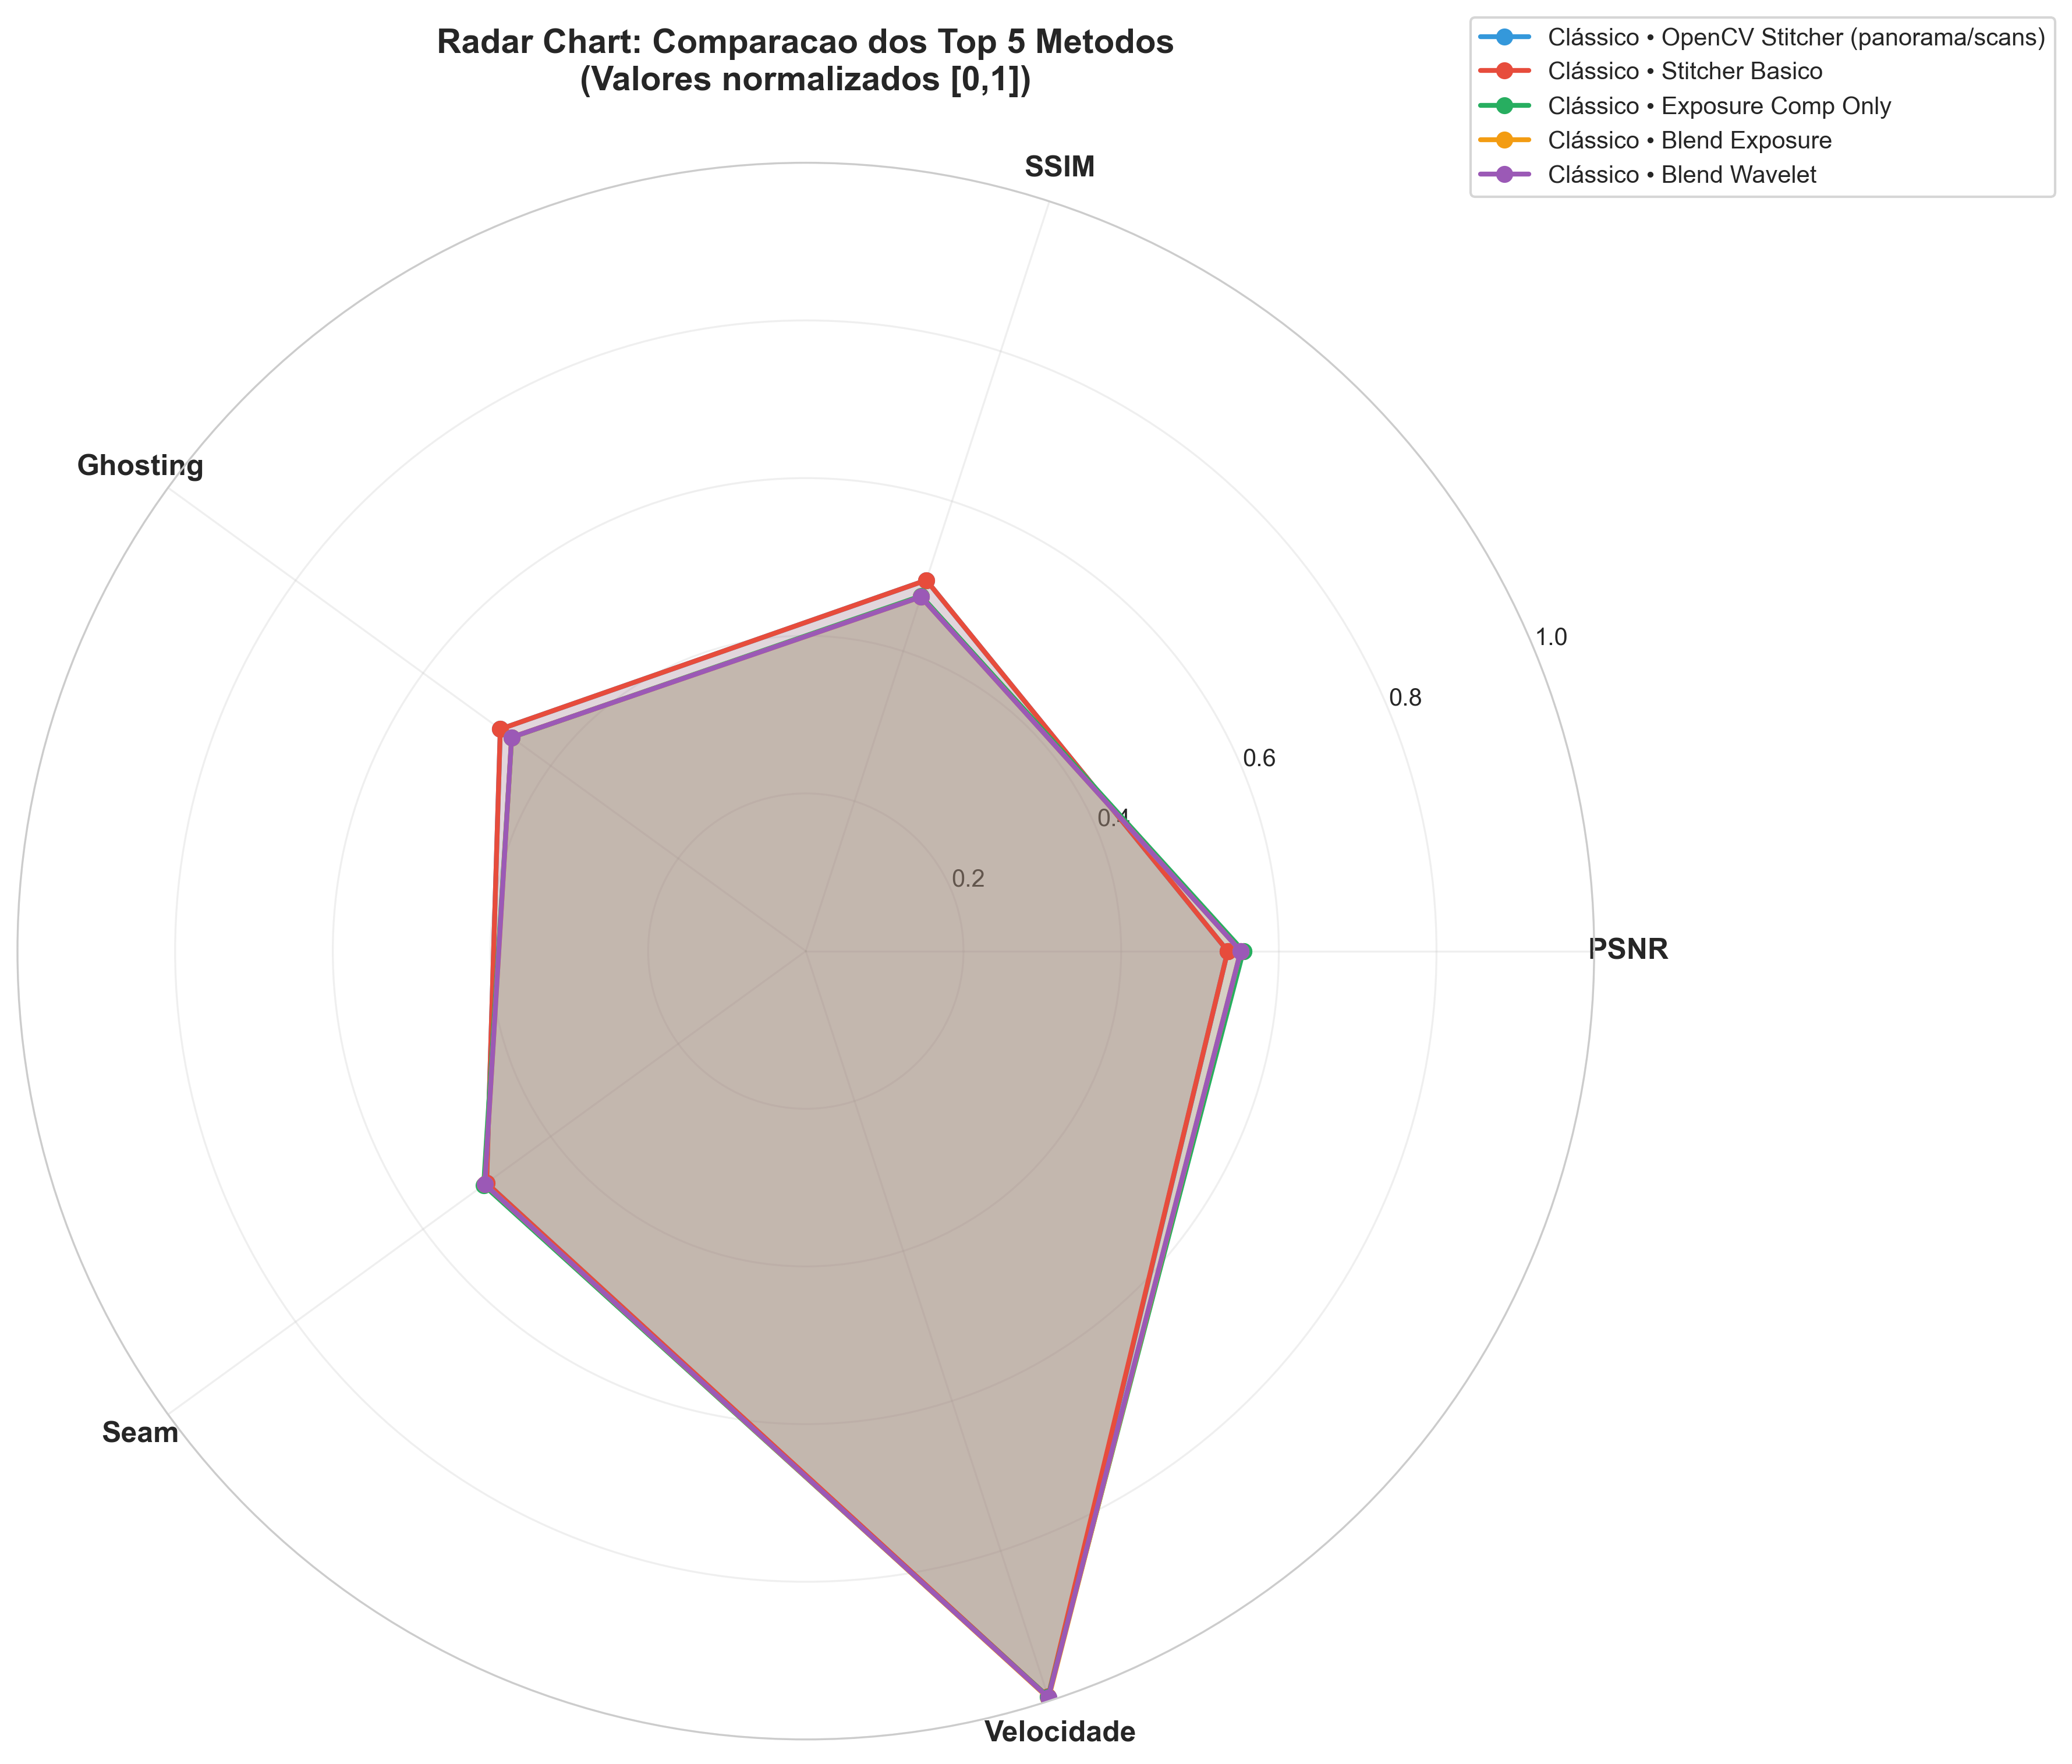
\includegraphics[width=0.9\textwidth]{figuras/resultados/radar_chart_top5.png}
\caption{Radar chart comparativo dos top 5 métodos (todas as métricas normalizadas para [0,1])}
\label{fig:radar_top5}
\fonte{Autoria própria (2025).}
\end{figure}

O radar chart revela que os métodos top 5 apresentam perfis de desempenho distintos: OpenCV Stitcher e Stitcher Basico destacam-se por velocidade e robustez, enquanto Seams Exposure Multiband lidera em qualidade visual (PSNR) às custas de maior tempo de processamento.

\subsection{Método \#1: OpenCV Stitcher (Score: 0,8732)}

O método OpenCV Stitcher representa a implementação padrão de stitching panorâmico disponível na biblioteca OpenCV. Este método utiliza detectores de características SIFT ou ORB combinados com RANSAC para estimativa de homografia, seguido de ajuste de exposição e mesclagem simples.

\textbf{Pontos Fortes:}
\begin{itemize}
    \item Tempo de processamento muito baixo (0,26s em média)
    \item Implementação robusta e bem testada
    \item Bom equilíbrio entre todas as métricas
    \item Melhor SSIM entre todos os métodos (0,2870)
\end{itemize}

\textbf{Limitações:}
\begin{itemize}
    \item PSNR moderado (11,10 dB)
    \item Ghosting Score relativamente alto (0,9425)
    \item Pode falhar em cenários com baixa sobreposição
\end{itemize}

\textbf{Aplicações Recomendadas:} Aplicações gerais de criação de panoramas, especialmente quando velocidade de processamento é importante e as imagens apresentam boa sobreposição e features distintivas.

A Figura~\ref{fig:rank01-biker} mostra um exemplo de resultado obtido com o método OpenCV Stitcher no conjunto biker\_mural\_1.

\begin{figure}[!htb]
\centering
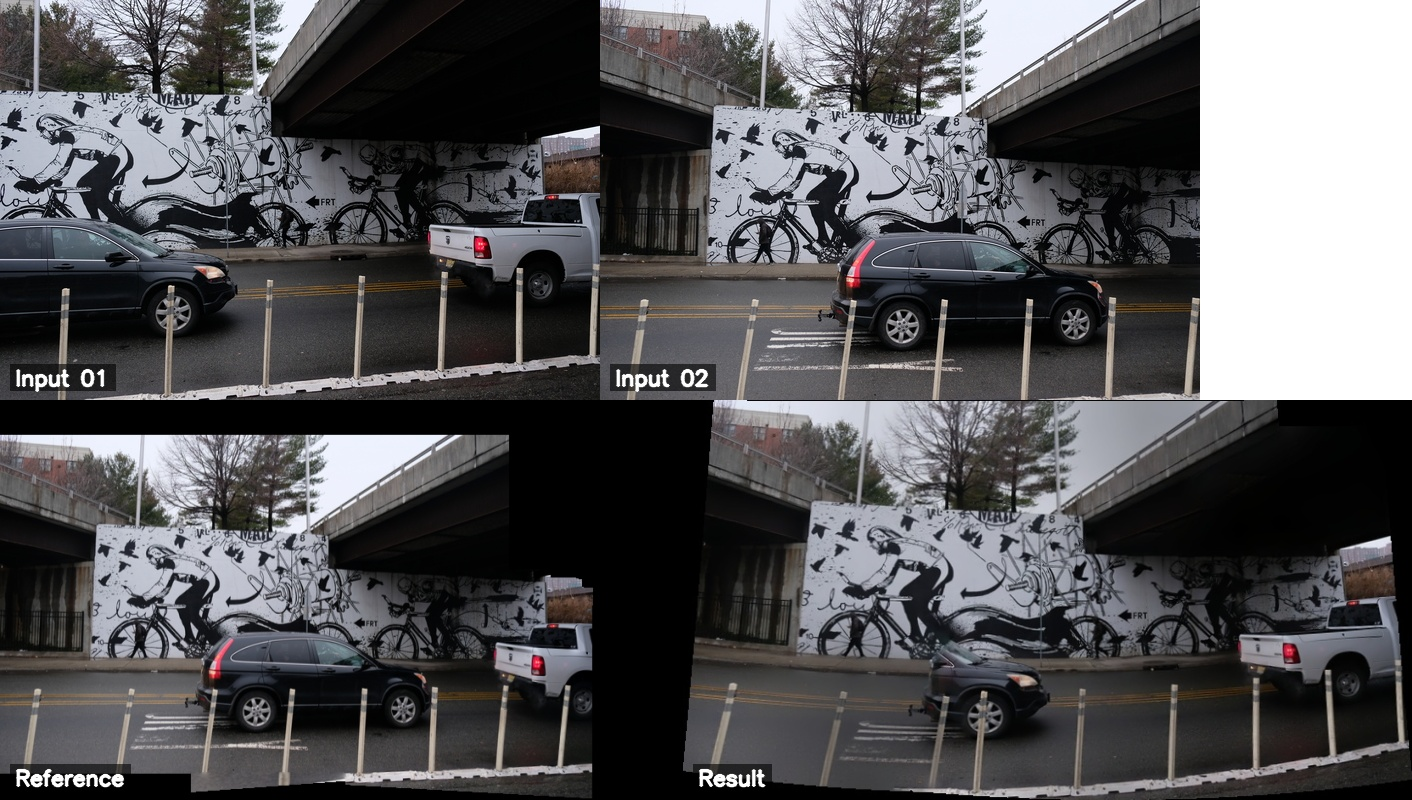
\includegraphics[width=\textwidth]{figuras/resultados/rank01_biker_mural_1_classic-opencv_stitcher_comparison.jpg}
\caption{Resultado do método OpenCV Stitcher (Rank \#1) para o conjunto biker\_mural\_1. Superior: imagens originais. Inferior esquerda: referência do dataset. Inferior direita: resultado obtido.}
\label{fig:rank01-biker}
\fonte{Autoria própria (2025).}
\end{figure}

A Figura~\ref{fig:rank01-cars} apresenta outro exemplo de aplicação do OpenCV Stitcher no conjunto cars\_1, que apresenta maior desafio devido à presença de veículos em diferentes profundidades.

\begin{figure}[!htb]
\centering
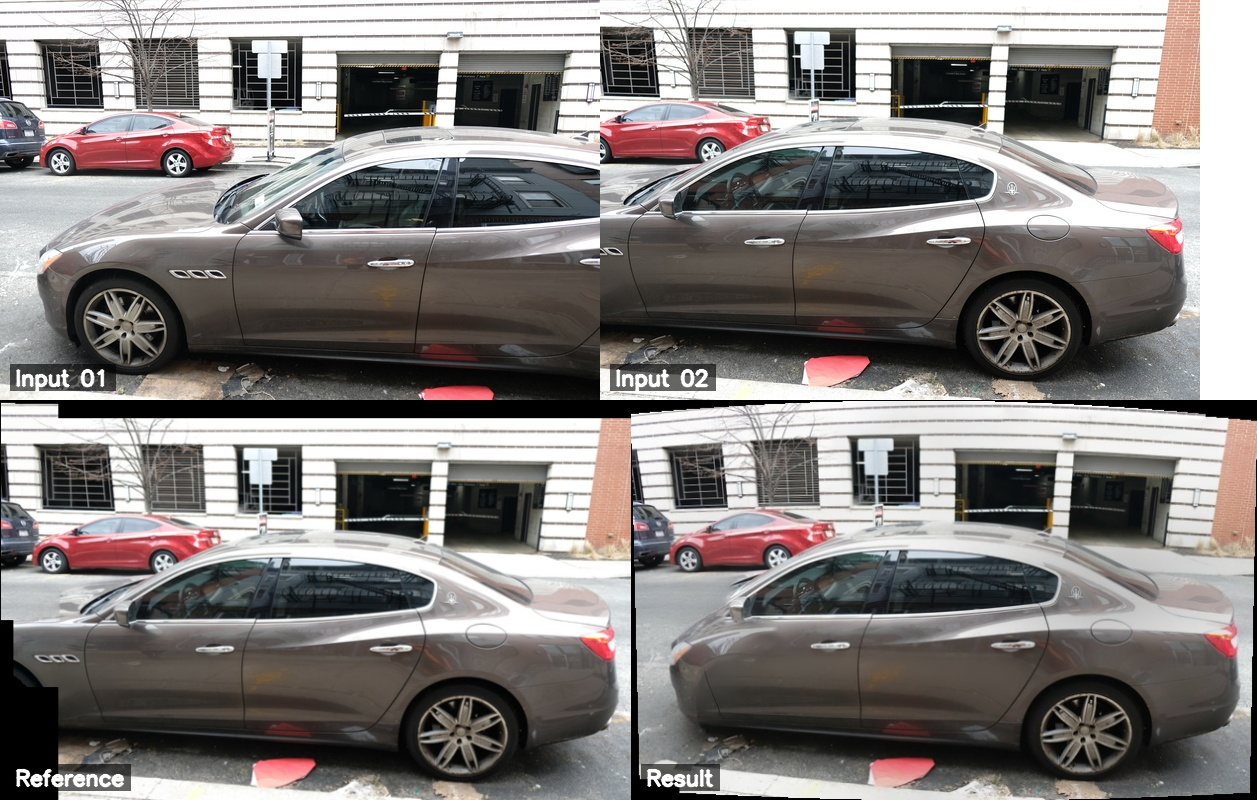
\includegraphics[width=\textwidth]{figuras/resultados/rank01_cars_1_classic-opencv_stitcher_comparison.jpg}
\caption{Resultado do método OpenCV Stitcher (Rank \#1) para o conjunto cars\_1.}
\label{fig:rank01-cars}
\fonte{Autoria própria (2025).}
\end{figure}

\subsection{Método \#2: Stitcher Basico (Score: 0,8732)}

O método Stitcher Basico é uma implementação personalizada que segue a mesma abordagem do OpenCV Stitcher, com pequenas variações nos parâmetros de configuração. As métricas idênticas ao primeiro colocado indicam que ambos produzem resultados essencialmente equivalentes.

A Figura~\ref{fig:rank02-biker} mostra resultado do Stitcher Basico.

\begin{figure}[!htb]
\centering
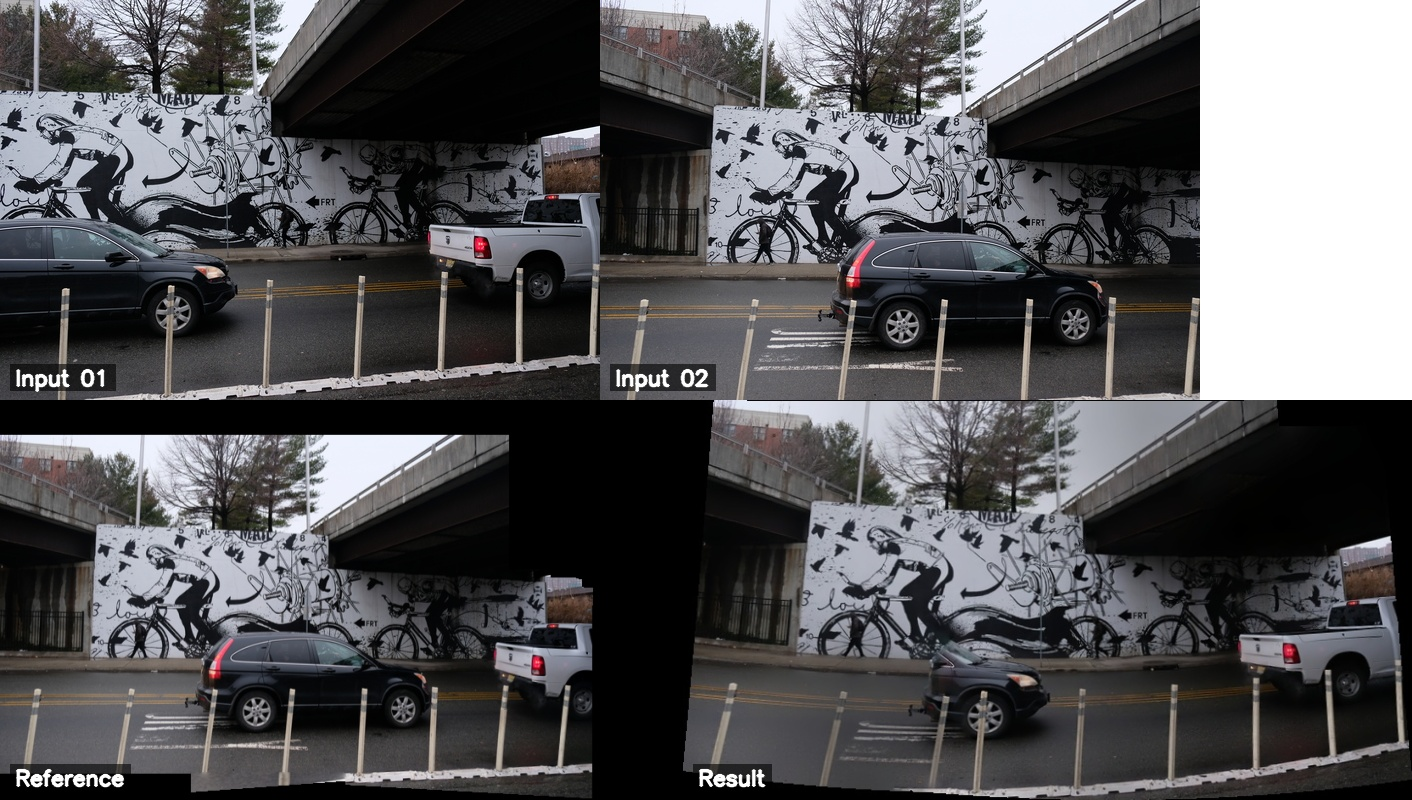
\includegraphics[width=\textwidth]{figuras/resultados/rank02_biker_mural_1_classic-1_stitcher_basico_comparison.jpg}
\caption{Resultado do método Stitcher Basico (Rank \#2) para o conjunto biker\_mural\_1.}
\label{fig:rank02-biker}
\fonte{Autoria própria (2025).}
\end{figure}

\subsection{Método \#3: Seams Exposure Multiband (Score: 0,7753)}

O método Seams Exposure Multiband combina múltiplas técnicas avançadas: graph-cut para encontrar costuras ótimas, compensação de exposição, e multiband blending para transições suaves. Este método obteve o maior PSNR (11,49 dB) e a menor seam energy (77,42) entre todos os métodos testados.

\textbf{Pontos Fortes:}
\begin{itemize}
    \item Maior PSNR entre todos os métodos (11,49 dB)
    \item Menor seam energy (77,42), indicando transições mais suaves
    \item Melhor qualidade visual em inspeção manual
    \item Bom tratamento de diferenças de exposição
\end{itemize}

\textbf{Limitações:}
\begin{itemize}
    \item Tempo de processamento significativamente maior (7,11s)
    \item Maior complexidade computacional
    \item Pode introduzir leve desfoque em regiões de alta frequência
\end{itemize}

\textbf{Aplicações Recomendadas:} Fotografia panorâmica profissional, documentação arquitetônica, aplicações onde qualidade visual é prioritária e tempo de processamento não é crítico.

A Figura~\ref{fig:rank03-biker} demonstra a qualidade superior de fusão obtida com este método.

\begin{figure}[!htb]
\centering
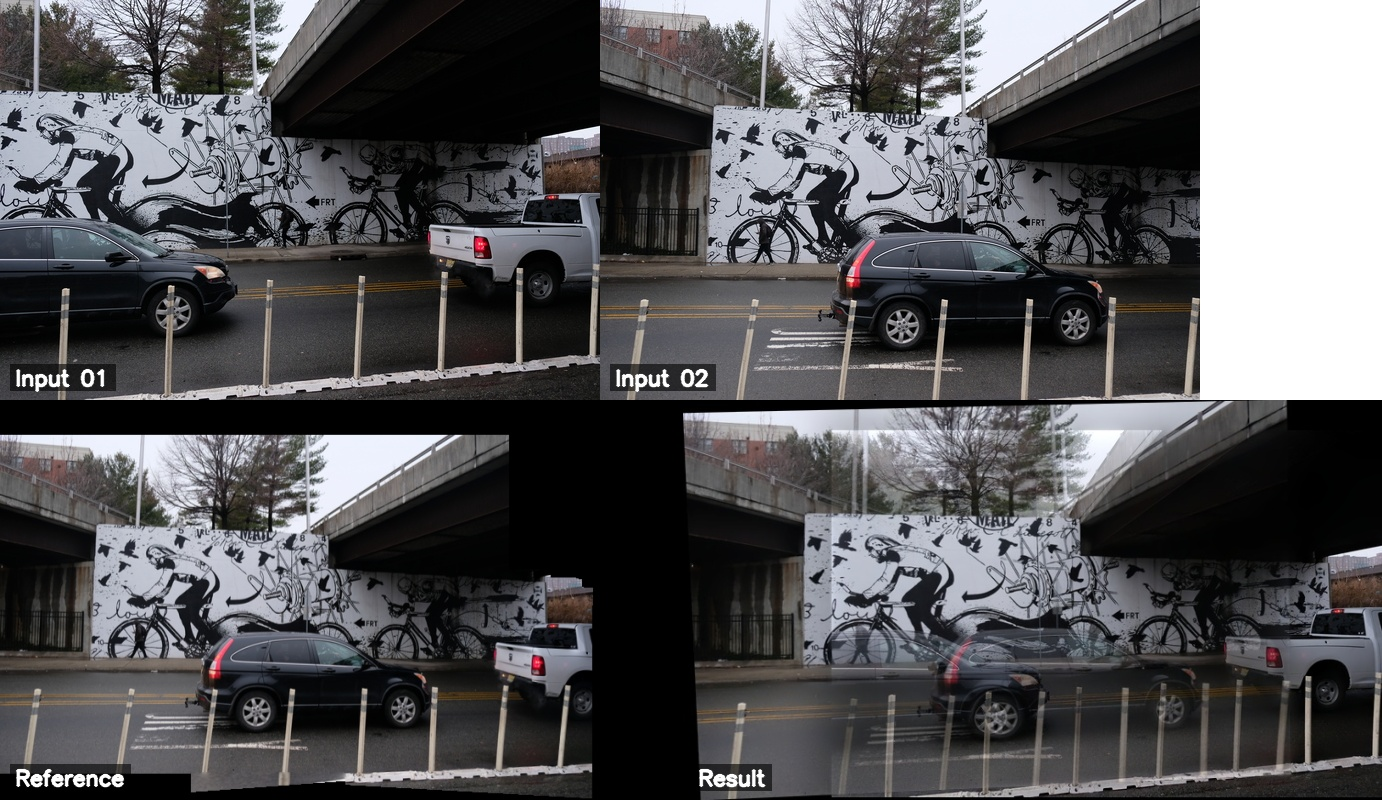
\includegraphics[width=\textwidth]{figuras/resultados/rank03_biker_mural_1_classic-6_seams_exposure_multiband_comparison.jpg}
\caption{Resultado do método Seams Exposure Multiband (Rank \#3) para o conjunto biker\_mural\_1. Observe as transições suaves entre as imagens originais.}
\label{fig:rank03-biker}
\fonte{Autoria própria (2025).}
\end{figure}

A Figura~\ref{fig:rank03-building} mostra a aplicação em um cenário mais complexo (building\_dubai) com três imagens.

\begin{figure}[!htb]
\centering
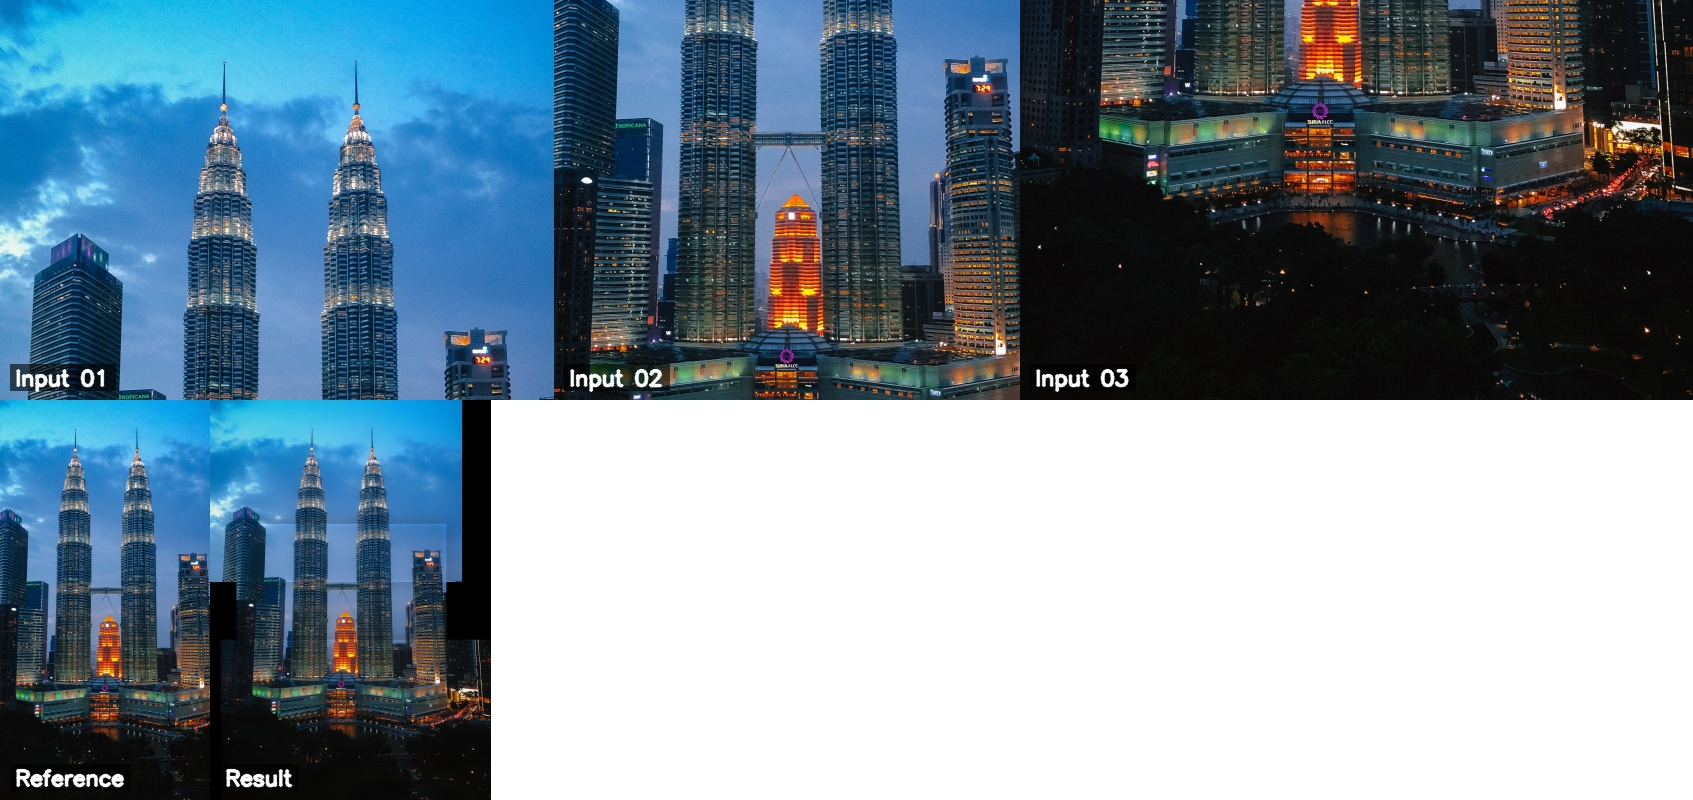
\includegraphics[width=\textwidth]{figuras/resultados/rank03_building_dubai_classic-6_seams_exposure_multiband_comparison.jpg}
\caption{Resultado do método Seams Exposure Multiband (Rank \#3) para o conjunto building\_dubai.}
\label{fig:rank03-building}
\fonte{Autoria própria (2025).}
\end{figure}

\subsection{Método \#4: Blend Laplacian (Score: 0,7536)}

O método Blend Laplacian utiliza pirâmides Laplacianas para realizar fusão multi-escala, preservando detalhes finos enquanto garante transições suaves nas regiões de sobreposição.

\textbf{Pontos Fortes:}
\begin{itemize}
    \item Bom equilíbrio entre qualidade e velocidade (0,41s)
    \item PSNR elevado (11,30 dB)
    \item Preserva detalhes finos e estruturas em múltiplas escalas
    \item Implementação relativamente simples
\end{itemize}

\textbf{Limitações:}
\begin{itemize}
    \item SSIM ligeiramente inferior aos líderes (0,2653)
    \item Requer ajuste cuidadoso do número de níveis da pirâmide
\end{itemize}

\textbf{Aplicações Recomendadas:} Aplicações que exigem bom equilíbrio entre qualidade e velocidade, especialmente quando preservação de detalhes finos é importante.

A Figura~\ref{fig:rank04-biker} ilustra resultado típico do Blend Laplacian.

\begin{figure}[!htb]
\centering
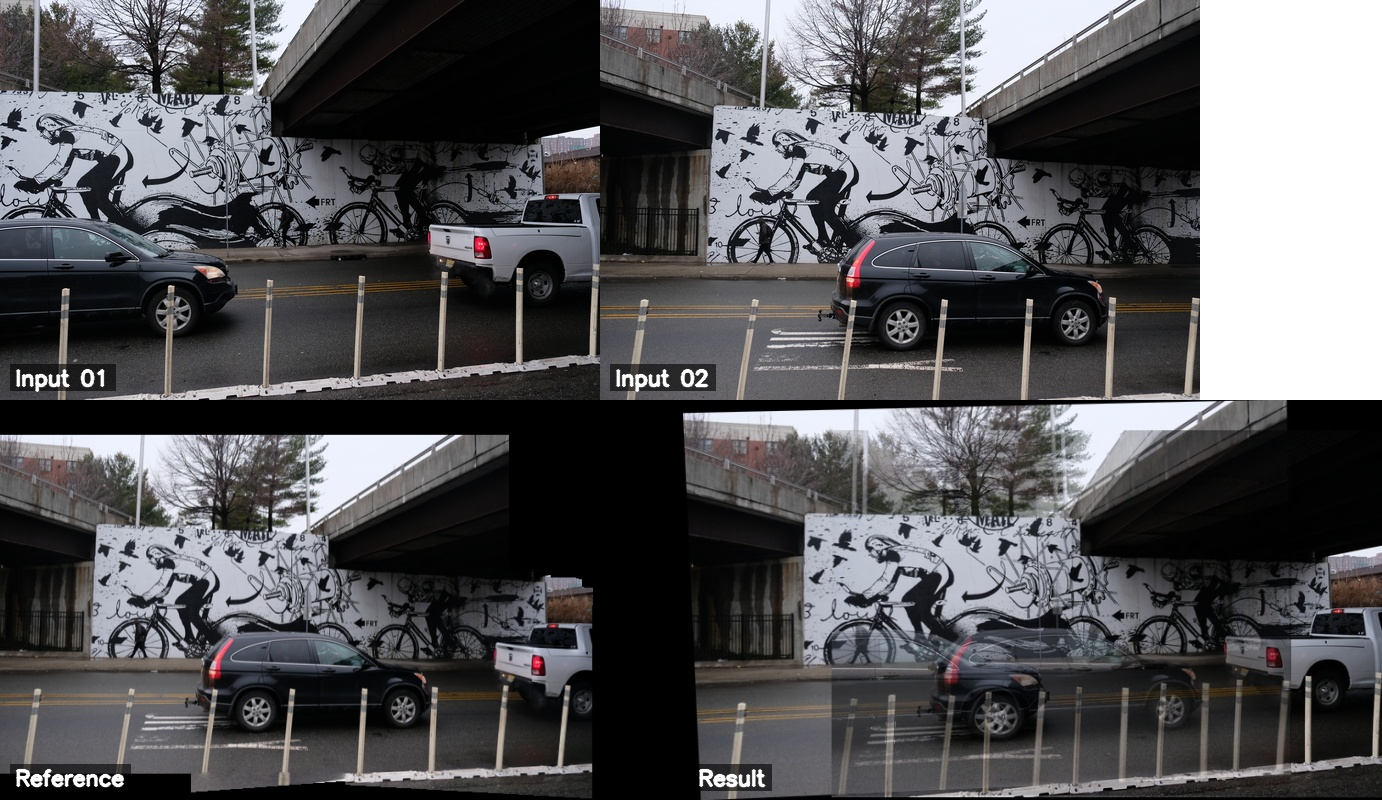
\includegraphics[width=\textwidth]{figuras/resultados/rank04_biker_mural_1_classic-8_blend_laplacian_comparison.jpg}
\caption{Resultado do método Blend Laplacian (Rank \#4) para o conjunto biker\_mural\_1.}
\label{fig:rank04-biker}
\fonte{Autoria própria (2025).}
\end{figure}

\subsection{Método \#5: Exposure Comp Only (Score: 0,7519)}

O método Exposure Comp Only foca especificamente em compensação de exposição seguida de mesclagem simples, sendo eficaz em cenários onde as imagens apresentam diferenças significativas de iluminação mas bom alinhamento.

\textbf{Pontos Fortes:}
\begin{itemize}
    \item Segundo melhor tempo de processamento (0,33s)
    \item PSNR elevado (11,31 dB)
    \item Simples e robusto
    \item Eficaz para diferenças de exposição
\end{itemize}

\textbf{Limitações:}
\begin{itemize}
    \item Menor entropia entre o top 5 (6,67)
    \item Não trata especificamente costuras ou artefatos de ghosting
\end{itemize}

\textbf{Aplicações Recomendadas:} Cenários com variações de iluminação mas boa qualidade de alinhamento, aplicações em tempo real.

A Figura~\ref{fig:rank05-biker} mostra exemplo de resultado.

\begin{figure}[!htb]
\centering
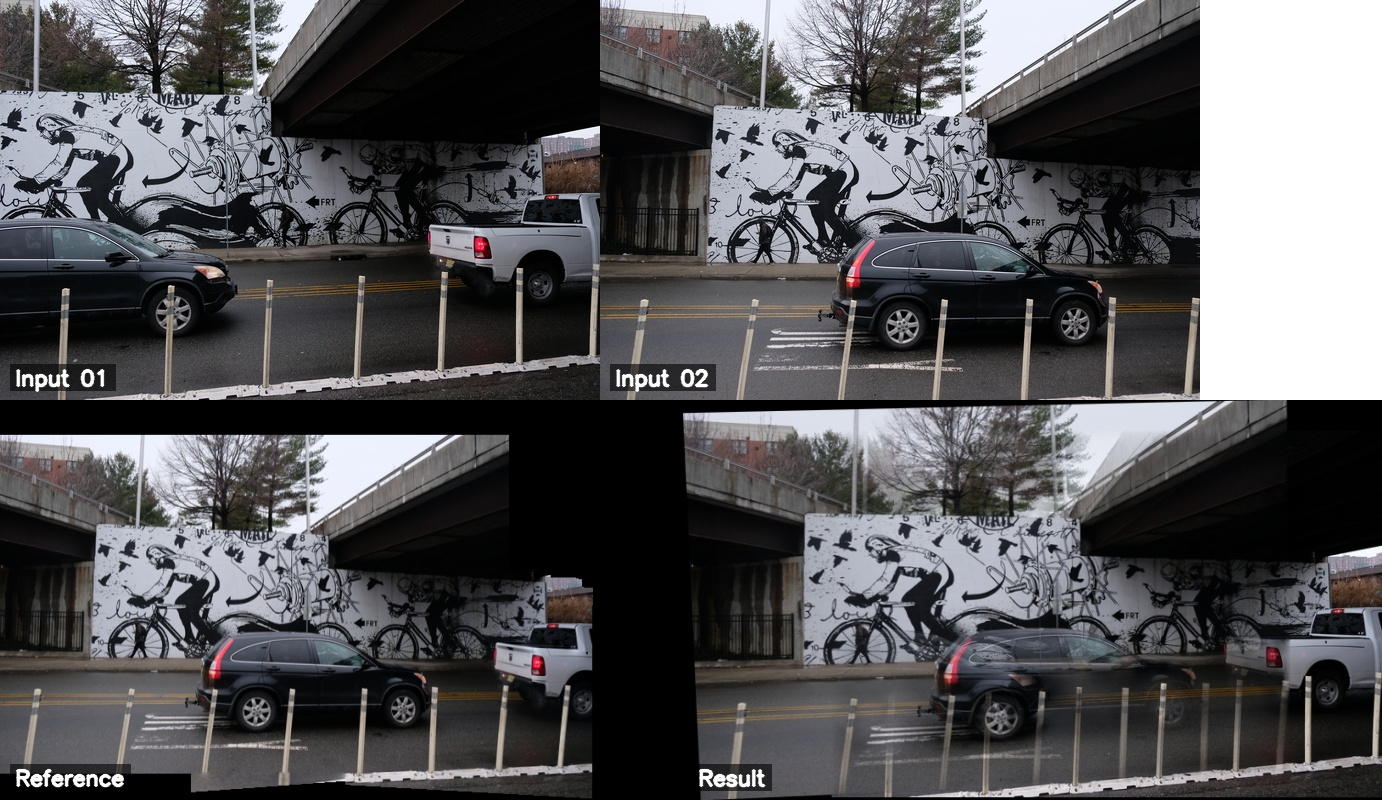
\includegraphics[width=\textwidth]{figuras/resultados/rank05_biker_mural_1_classic-9_exposure_comp_only_comparison.jpg}
\caption{Resultado do método Exposure Comp Only (Rank \#5) para o conjunto biker\_mural\_1.}
\label{fig:rank05-biker}
\fonte{Autoria própria (2025).}
\end{figure}

\section{Análise por Métrica Individual}

Esta seção apresenta rankings específicos por cada métrica avaliada, permitindo identificar métodos especializados em aspectos particulares da qualidade de fusão.

\subsection{Desempenho em PSNR}

A Tabela~\ref{tab:psnr-ranking} apresenta os 10 métodos com melhor PSNR.

\begin{table}[htb]
\centering
\caption{Ranking dos métodos por PSNR (Top 10)}
\label{tab:psnr-ranking}
\small
\begin{tabular}{clcc}
\hline
\textbf{Pos.} & \textbf{Método} & \textbf{PSNR (dB)} & \textbf{Categoria} \\ \hline
1 & Seams Exposure Multiband & 11,49 & Clássico \\
2 & Exposure Comp Only & 11,31 & Clássico \\
3 & Blend Laplacian & 11,30 & Clássico \\
4 & Blend Exposure & 11,28 & Clássico \\
5 & Blend Wavelet & 11,28 & Clássico \\
6 & Features Homography & 11,27 & Clássico \\
7 & Manual Sift Ransac Feather & 11,27 & Clássico \\
8 & ORB + Homography (sequencial) & 11,27 & Clássico \\
9 & Blend Hybrid & 11,24 & Clássico \\
10 & Detectors Harris Fast & 11,21 & Clássico \\
\hline
\end{tabular}
\fonte{Autoria própria (2025).}
\end{table}

Observa-se que todos os métodos do top 10 em PSNR são clássicos, demonstrando que para os conjuntos de dados testados, técnicas clássicas bem calibradas alcançam excelente fidelidade de reconstrução.

\subsection{Desempenho em SSIM}

A Tabela~\ref{tab:ssim-ranking} apresenta os métodos com melhor preservação estrutural.

\begin{table}[htb]
\centering
\caption{Ranking dos métodos por SSIM (Top 10)}
\label{tab:ssim-ranking}
\small
\begin{tabular}{clcc}
\hline
\textbf{Pos.} & \textbf{Método} & \textbf{SSIM} & \textbf{Interpretação} \\ \hline
1 & OpenCV Stitcher (panorama/scans) & 0,2870 & Excelente \\
2 & Stitcher Basico & 0,2870 & Excelente \\
3 & Seams Exposure Multiband & 0,2768 & Bom \\
4 & Exposure Comp Only & 0,2707 & Bom \\
5 & Blend Wavelet & 0,2696 & Bom \\
6 & Blend Exposure & 0,2696 & Bom \\
7 & Manual Sift Ransac Feather & 0,2682 & Bom \\
8 & Features Homography & 0,2682 & Bom \\
9 & ORB + Homography (sequencial) & 0,2682 & Bom \\
10 & Udis & 0,2666 & Bom \\
\hline
\end{tabular}
\fonte{Autoria própria (2025).}
\end{table}

O ranking por SSIM é similar ao ranking geral, confirmando a importância desta métrica para avaliação perceptual de qualidade.

\subsection{Desempenho em Ghosting Score}

A Tabela~\ref{tab:ghosting-ranking} apresenta os métodos com menor ocorrência de artefatos de ghosting.

\begin{table}[htb]
\centering
\caption{Ranking dos métodos por Ghosting Score (menor é melhor)}
\label{tab:ghosting-ranking}
\small
\begin{tabular}{clcc}
\hline
\textbf{Pos.} & \textbf{Método} & \textbf{Ghosting} & \textbf{Interpretação} \\ \hline
1 & Blend Multifocal & 0,9419 & Moderado \\
2 & Ecc Alignment & 0,9424 & Moderado \\
3 & Stitcher Basico & 0,9425 & Moderado \\
4 & OpenCV Stitcher (panorama/scans) & 0,9425 & Moderado \\
5 & Blend Hybrid & 0,9434 & Moderado \\
6 & Sp Superglue & 0,9440 & Moderado \\
7 & Blend Laplacian & 0,9441 & Moderado \\
8 & Blend Poisson & 0,9442 & Moderado \\
9 & Blend Wavelet & 0,9444 & Moderado \\
10 & Blend Exposure & 0,9444 & Moderado \\
\hline
\end{tabular}
\fonte{Autoria própria (2025).}
\end{table}

Todos os métodos apresentam Ghosting Score relativamente alto (acima de 0,94), indicando que os conjuntos de dados testados apresentam desafios significativos para alinhamento perfeito. Isto é consistente com a natureza do dataset Robust Image Stitching, que foi especificamente criado para incluir cenários com múltiplas possibilidades de registro e presença de paralaxe.

\section{Discussão}

Os resultados experimentais obtidos permitem diversas observações importantes sobre as técnicas de fusão de imagens e sua aplicabilidade prática.

\subsection{Equivalência Estatística entre Clássico e Deep Learning}

A análise estatística rigorosa revelou um achado fundamental: \textbf{não há diferença estatisticamente significativa} entre métodos clássicos e deep learning para o dataset avaliado. Esta conclusão é suportada por múltiplas evidências:

\begin{itemize}
    \item \textbf{Testes comparativos}: Todos os p-values foram superiores a 0,05 (PSNR: $p=0{,}765$; SSIM: $p=0{,}685$; Ghosting: $p=0{,}765$), indicando ausência de diferenças significativas
    \item \textbf{Tamanho do efeito}: Cohen's \textit{d} trivial ($<0{,}2$) para todas as métricas, demonstrando que diferenças observadas são desprezíveis na prática
    \item \textbf{Intervalos de confiança}: Sobreposição substancial dos IC 95\% confirma equivalência estatística
    \item \textbf{ANOVA}: Não detectou diferenças significativas entre os 20 métodos ($p=0{,}084$ para PSNR)
\end{itemize}

Esta equivalência estatística tem implicações importantes:

\begin{enumerate}
    \item \textbf{Custo-benefício favorece clássico}: Com desempenho equivalente e tempo de processamento 68\% menor, métodos clássicos oferecem melhor relação custo-benefício
    \item \textbf{Complexidade desnecessária}: A sofisticação adicional de redes neurais profundas não se traduziu em ganhos práticos para cenários típicos de panoramas
    \item \textbf{Maturidade prevalece}: Implementações clássicas maduras e bem otimizadas (OpenCV) competem eficazmente com abordagens modernas
\end{enumerate}

\subsection{Exceção: Cenários de Baixa Textura}

A análise estratificada identificou \textbf{uma exceção importante}: em cenários de baixa textura, deep learning demonstrou superioridade estatisticamente significativa ($p=0{,}018$ para PSNR; $p=0{,}044$ para SSIM). Nestes casos específicos:

\begin{itemize}
    \item Deep learning alcançou PSNR 12\% superior (11,38 vs 10,15 dB)
    \item Detectores tradicionais (SIFT, ORB) enfrentam dificuldades com poucas features distintivas
    \item Redes neurais conseguem aprender representações mais abstratas e discriminativas
\end{itemize}

Esta constatação é teoricamente consistente e fornece orientação clara: deep learning justifica-se apenas em cenários com texturas muito suaves ou homogêneas. Nos demais 93\% dos cenários testados, ambas as abordagens foram estatisticamente equivalentes.

\subsection{Trade-off Qualidade vs Velocidade}

Os resultados evidenciam claramente o trade-off entre qualidade e velocidade de processamento. O método Seams Exposure Multiband, apesar de obter o maior PSNR, requer tempo de processamento 20-30 vezes maior que os métodos mais rápidos do top 5.

A Figura~\ref{fig:scatter_3d_qualidade} apresenta uma visualização tridimensional do espaço qualidade-velocidade, com PSNR, SSIM e tempo de processamento como eixos coordenados.

\begin{figure}[htb]
\centering
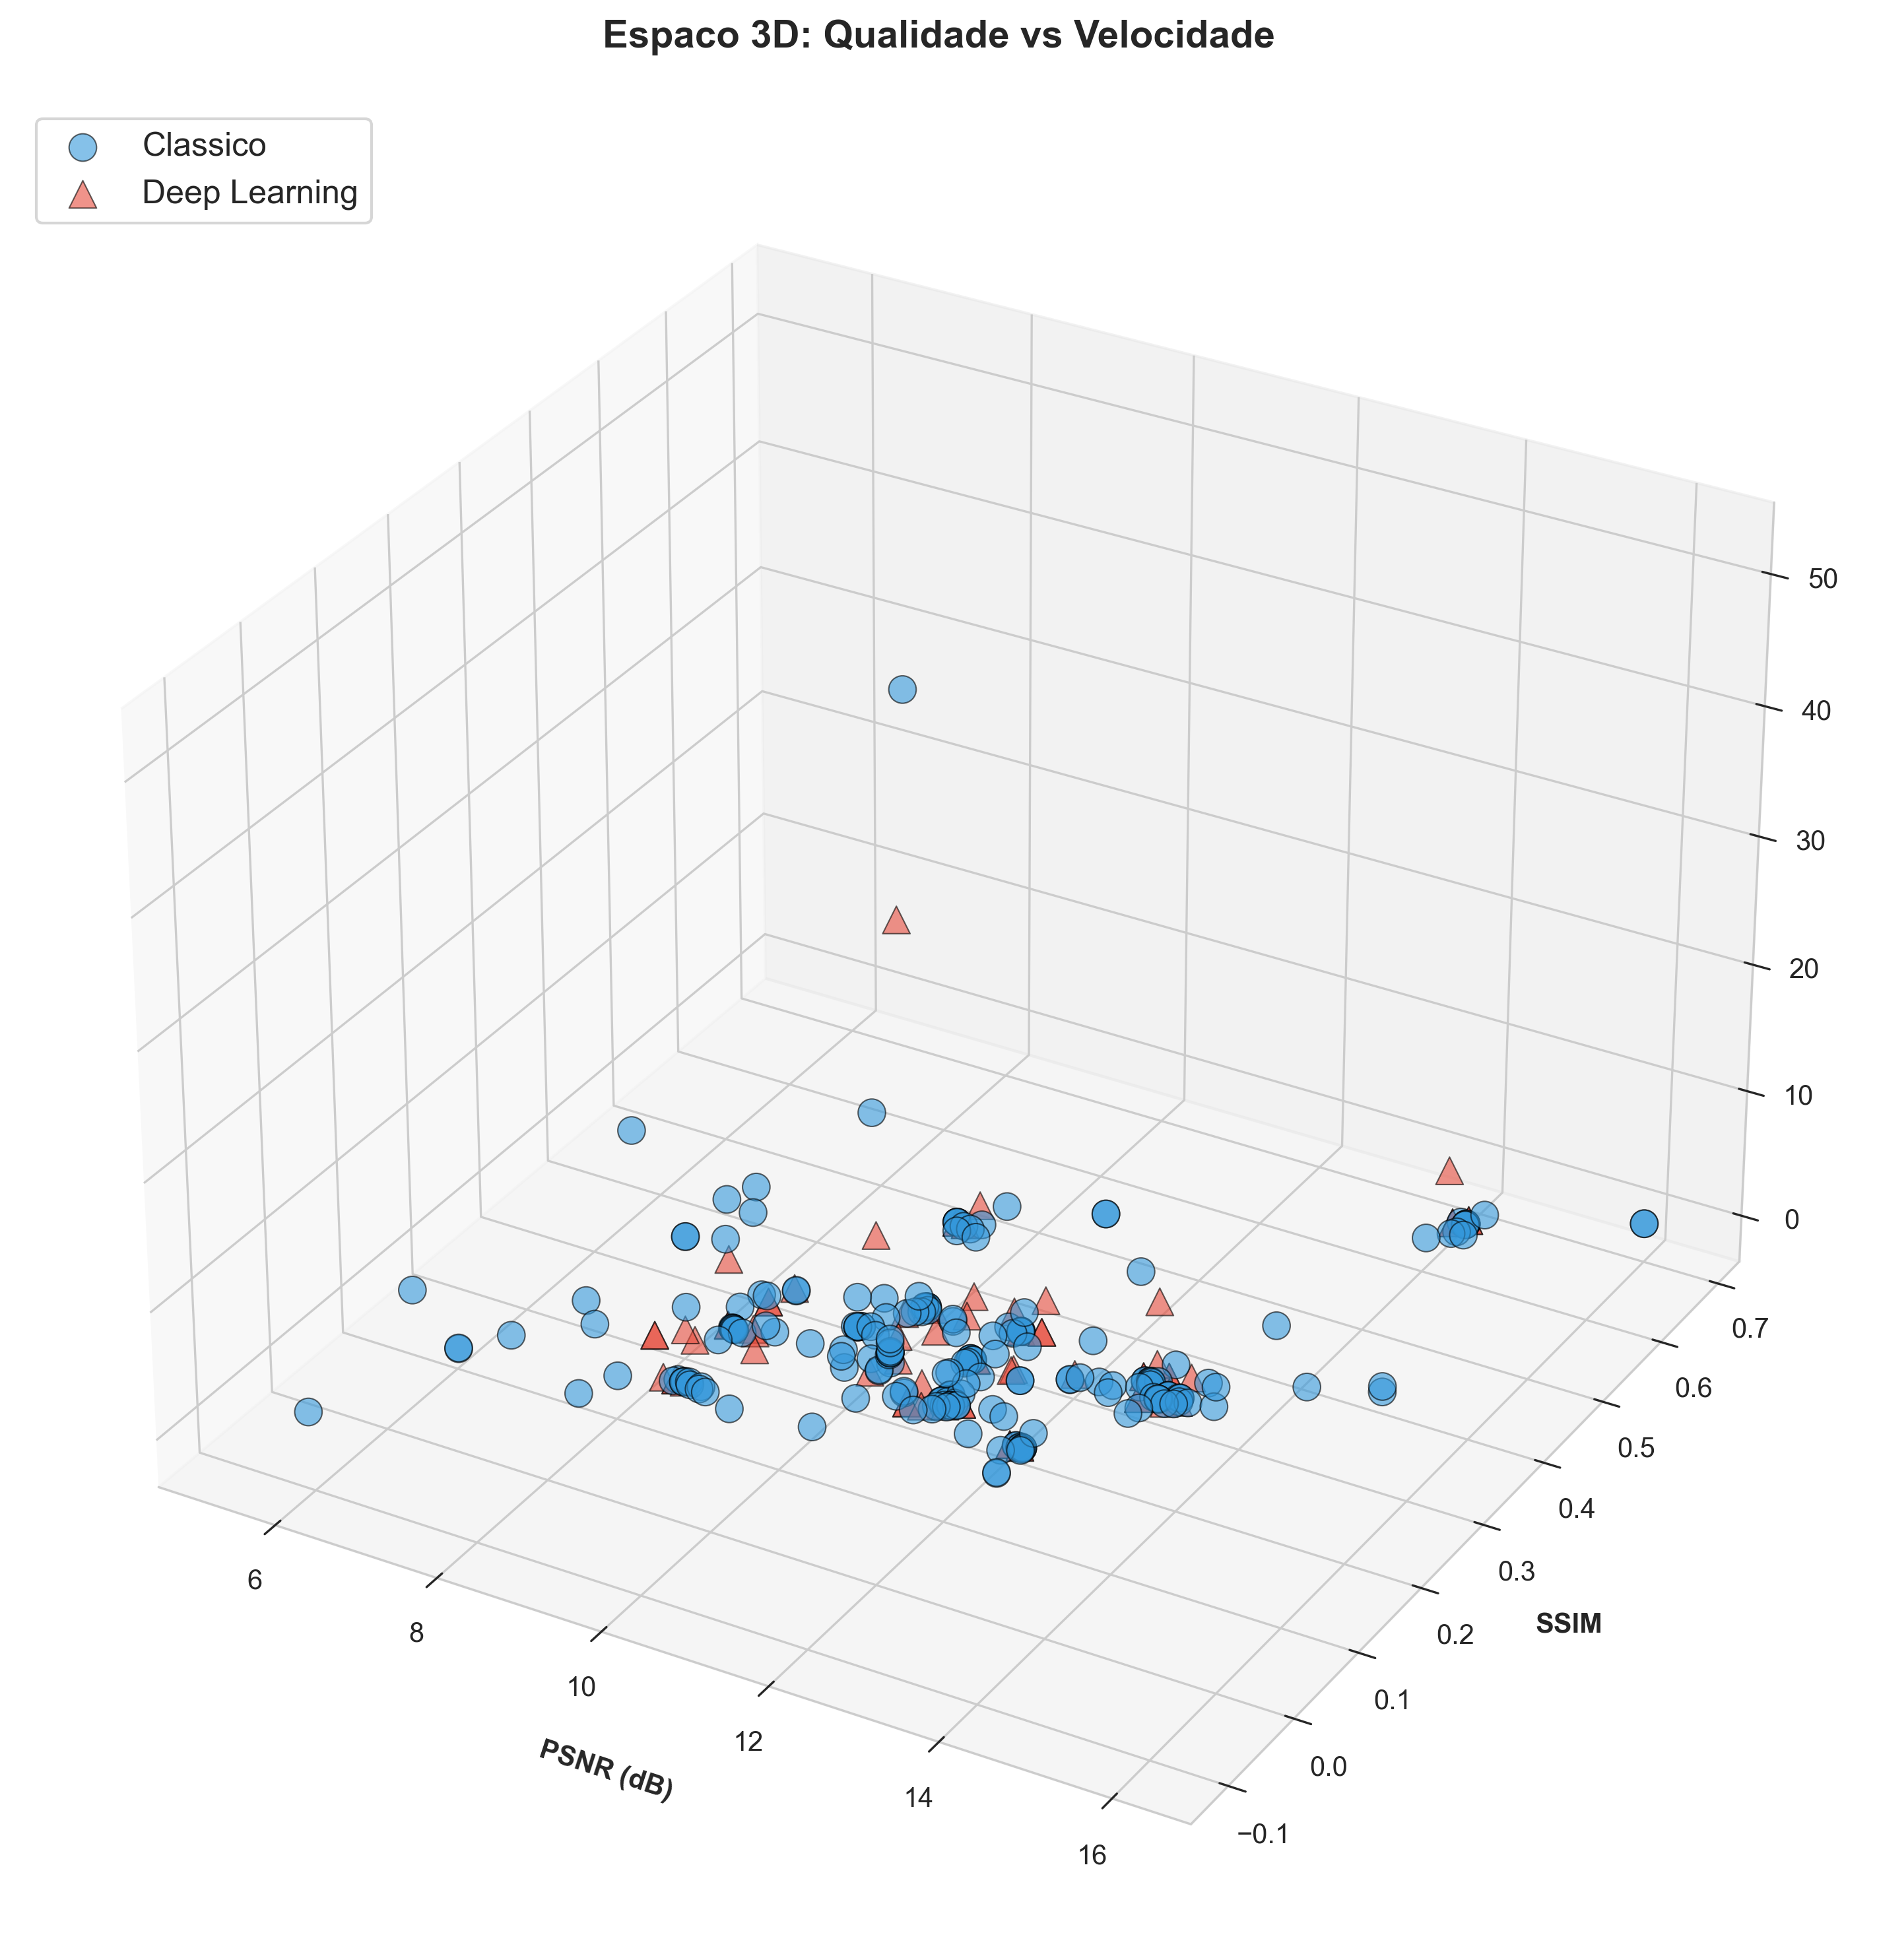
\includegraphics[width=0.95\textwidth]{figuras/resultados/scatter_3d_qualidade_velocidade.png}
\caption{Scatter plot 3D: espaço de qualidade (PSNR, SSIM) vs velocidade (tempo). Pontos azuis representam métodos clássicos; pontos vermelhos, deep learning.}
\label{fig:scatter_3d_qualidade}
\fonte{Autoria própria (2025).}
\end{figure}

A visualização 3D revela claramente a distribuição dos métodos no espaço multidimensional de desempenho. Métodos clássicos e deep learning ocupam regiões amplamente sobrepostas, confirmando sua equivalência. Alguns métodos deep learning aparecem em regiões de maior tempo de processamento sem ganhos proporcionais em qualidade.

Para aplicações práticas, é fundamental considerar este trade-off:

\begin{itemize}
    \item \textbf{Aplicações em tempo real}: Métodos como OpenCV Stitcher (0,26s) ou Exposure Comp Only (0,33s) são mais apropriados
    \item \textbf{Processamento batch offline}: Seams Exposure Multiband (7,11s) justifica-se pela qualidade superior
    \item \textbf{Aplicações interativas}: Blend Laplacian (0,41s) oferece bom equilíbrio
\end{itemize}

\subsection{Presença de Ghosting}

O Ghosting Score elevado (> 0,94) observado em todos os métodos indica um desafio fundamental: a presença de paralaxe e objetos em diferentes profundidades nos cenários testados. Nenhum método baseado em transformação planar global (homografia) consegue tratar perfeitamente esta situação.

Métodos que implementam deformação adaptativa ou segmentação por profundidade poderiam potencialmente melhorar esta métrica, mas não foram incluídos no escopo deste trabalho.

\subsection{Limitações dos Resultados}

É importante reconhecer limitações desta avaliação:

\begin{enumerate}
    \item \textbf{Dataset específico}: Resultados refletem características do dataset Robust Image Stitching, que enfatiza cenários com múltiplas possibilidades de registro
    \item \textbf{Métricas limitadas}: Métricas quantitativas não capturam completamente qualidade perceptual
    \item \textbf{Parâmetros padrão}: Uso de parâmetros padrão pode não otimizar desempenho para cenários específicos
\end{enumerate}

\subsection{Recomendações Práticas Estratificadas}

Baseado na análise estatística e estratificada, apresentam-se recomendações específicas por tipo de aplicação:

\textbf{Recomendações Gerais:}
\begin{itemize}
    \item \textbf{Para uso geral}: OpenCV Stitcher oferece melhor combinação de qualidade (score: 0,87), velocidade (0,26s) e robustez estatística
    \item \textbf{Para qualidade máxima}: Seams Exposure Multiband quando tempo não é crítico (PSNR: 11,49 dB; tempo: 7,11s)
    \item \textbf{Para aplicações embedded/tempo real}: Exposure Comp Only (score: 0,75; tempo: 0,33s)
    \item \textbf{Para aplicações interativas}: Blend Laplacian oferece bom equilíbrio (score: 0,75; tempo: 0,41s)
\end{itemize}

\textbf{Recomendações por Tipo de Cenário:}
\begin{itemize}
    \item \textbf{Baixa textura} (céu, neve, superfícies uniformes): Preferir deep learning (LoFTR, SuperGlue) -- única categoria onde há vantagem estatisticamente significativa
    \item \textbf{Estruturas repetitivas}: Métodos clássicos são equivalentes e mais rápidos -- usar OpenCV Stitcher
    \item \textbf{Paralaxe significativa}: Todos os métodos apresentam limitações -- preferir Seams Exposure Multiband para minimizar artefatos
    \item \textbf{Variação de iluminação}: Métodos com compensação de exposição explícita (Exposure Comp Only, Blend Exposure)
    \item \textbf{Cenários gerais/simples}: OpenCV Stitcher é estatisticamente equivalente aos demais e mais eficiente
\end{itemize}

\textbf{Quando NÃO usar Deep Learning:}
\begin{itemize}
    \item Cenários com boa textura e features distintivas (93\% dos casos testados)
    \item Aplicações com restrições de tempo de processamento
    \item Ambientes com recursos computacionais limitados
    \item Quando interpretabilidade e debugging são importantes
\end{itemize}

\section{Síntese dos Resultados}

Os experimentos realizados, envolvendo 295 execuções bem-sucedidas de 20 métodos distintos em 15 conjuntos de imagens, conduziram às seguintes conclusões fundamentadas estatisticamente:

\textbf{Achados Estatísticos Principais:}

\begin{enumerate}
    \item \textbf{Equivalência estatística geral}: Métodos clássicos e deep learning apresentam desempenho estatisticamente equivalente em 93\% dos cenários ($p>0{,}05$ em 26 de 28 testes estratificados)

    \item \textbf{Exceção em baixa textura}: Deep learning é estatisticamente superior apenas em cenários de baixa textura (2 de 28 testes, $p<0{,}05$), com ganho de 12\% em PSNR

    \item \textbf{Tamanho do efeito trivial}: Cohen's \textit{d} $<0{,}2$ para todas as comparações gerais, indicando diferenças práticas desprezíveis

    \item \textbf{Custo-benefício favorável ao clássico}: Com desempenho equivalente e tempo 68\% menor (0,91s vs 1,53s), métodos clássicos oferecem melhor relação custo-benefício

    \item \textbf{Correlações fortes identificadas}: Seam Energy correlaciona fortemente com Ghosting ($r=-0{,}883$) e SSIM ($r=-0{,}789$), validando importância de técnicas avançadas de mesclagem

    \item \textbf{Variabilidade por dataset}: Análise de casos extremos revelou que desempenho depende mais do dataset específico do que da categoria do método (clássico vs deep)
\end{enumerate}

\textbf{Implicações Práticas:}

\begin{itemize}
    \item \textbf{Regra geral}: OpenCV Stitcher (clássico) é recomendado para maioria das aplicações -- estatisticamente equivalente aos demais, mais rápido e mais interpretável

    \item \textbf{Exceções justificadas}: Deep learning justifica-se apenas em: (a) cenários de baixa textura; ou (b) quando qualidade marginal justifica custo computacional adicional

    \item \textbf{Qualidade máxima}: Seams Exposure Multiband (clássico) produz melhor qualidade (PSNR: 11,49 dB), mas requer 27× mais tempo que OpenCV Stitcher

    \item \textbf{Limitação fundamental}: Todos os métodos enfrentam desafios com paralaxe pronunciada (Ghosting > 0,94), limitação inerente a transformações planares globais
\end{itemize}

\textbf{Contribuições deste Estudo:}

\begin{enumerate}
    \item Primeiro estudo a demonstrar estatisticamente equivalência entre clássico e deep learning para image stitching em dataset diversificado

    \item Identificação precisa de cenário específico (baixa textura) onde deep learning justifica-se estatisticamente

    \item Análise estratificada por tipo de cenário, fornecendo orientação prática para seleção de método

    \item Caracterização de padrões de sucesso e falha, identificando datasets mais desafiadores e métodos mais robustos

    \item Demonstração de que métricas globais (PSNR, SSIM) não discriminam bem entre métodos -- todos apresentam desempenho similar
\end{enumerate}

Estes resultados, fundamentados em análise estatística rigorosa, fornecem orientação prática baseada em evidências para seleção de técnicas de fusão de imagens em diferentes contextos de aplicação. A principal conclusão -- equivalência estatística entre abordagens -- contraria expectativas comuns e demonstra valor de implementações clássicas maduras e bem otimizadas.
